\documentclass[10pt,a4paper]{article}
%\documentclass[11pt,a4paper]{article}
%\documentclass[11pt,a4paper,draft]{article}
%\documentclass[11pt,twoside,a4paper]{article}

\usepackage[top=2cm, bottom=2cm, inner=2.5cm,   outer=2.5cm]{geometry}
%LaTeX's margins are, by default, 1.5 inches wide on 12pt documents, 1.75 inches wide on 11pt documents, and 1.875 inches wide on 10pt documents. This is the standard for book margins.


\usepackage[utf8]{inputenc}
\usepackage[T1]{fontenc}

\usepackage{amsmath,amsfonts,amssymb}
\usepackage{mathdots ,mathtools }
\usepackage{xfrac} % format maths
\usepackage{bm} % format maths
\usepackage{cancel} % lettes barrees
 
\usepackage{graphicx}

\usepackage[colorlinks,backref,citecolor=darkgray,linkcolor=darkgray]{hyperref}
%\usepackage{hyperref}
%\usepackage[hidelinks]{hyperref}
%\usepackage[colorlinks]{hyperref}
%\usepackage[colorlinks,backref ]{hyperref}

\usepackage{cases} % format equation This provides a LATEX environment {numcases} to produce multi-case equations with a separate equation number for each case.

\usepackage{enumitem}

\usepackage{booktabs} % To thicken table lines

\usepackage{array} % améliore grandement la qualité des tableaux sous LaTeX. La fiche au format pdf 

\usepackage{multirow,makecell} % format tables
\setcellgapes{1pt}
\makegapedcells
\newcolumntype{R}[1]{>{\raggedleft\arraybackslash }b{#1}}
\newcolumntype{L}[1]{>{\raggedright\arraybackslash }b{#1}}
\newcolumntype{C}[1]{>{\centering\arraybackslash }b{#1}}

%ASasaSA
%asAS
%ASasA

%biblio 
\usepackage{natbib} 
%\usepackage[round]{natbib} 
%\bibliographystyle{plain} % numero
%\bibliographystyle{plainnat}  %nom et anee
\bibliographystyle{apalike}  %nom et anee

\usepackage{caption}
\usepackage{subcaption}

\usepackage{enumitem}

%affiliations
\usepackage{authblk} % affiliation auteurs
\author[1,2]{Christophe Coste}
\author[2]{Samuel Pavard}
\affil[1]{\small MNHN \normalsize} 
\affil[2]{\small NTNU}

%date
\date{\today}

%raccourcis
\newcommand{\M}{$\mathbf{M}$}
\newcommand{\Magerf}{$\mathbf{M_{age,rf}}$} 
\newcommand{\Mage}{$\mathbf{M_{age}}$} 
\newcommand{\lam}{$\lambda$} 
\newcommand{\w}{$\mathbf{w}$} 
\newcommand{\Rzero}{$\boldsymbol{\mathcal{R}_{0}}$  } 
\newcommand{\LRO}{$\mathcal{LRS}$} 
%\newcommand{\PCoR}{\emph{individual component} of the costs} 
%\newcommand{\GCoR}{\emph{genetic component} of the costs} 
\newcommand{\PCoR}{\emph{individual} costs} 
\newcommand{\GCoR}{\emph{genetic} costs} 
\newcommand{\PCoRwgb}{costs of reproduction} 
\newcommand{\TLA}{Trait Level Analysis} 
\newcommand{\chapii}{\citep{Coste2017}} 
\newcommand{\Ma}{$\mathbf{M^{fold}_{age}}$} 
\newcommand{\Map}{$\mathbf{M^{fold}_{age,parity}}$} 
\newcommand{\Mah}{$\mathbf{M^{fold}_{age,strategy}}$} 
\newcommand{\vLRO}{$\sigma_{\mathrm{\mathcal{LRS}}}^2$} 
\newcommand{\vd}{$\sigma_{\mathrm{d}}^2$} 
\newcommand{\ve}{$\sigma_{\mathrm{e}}^2$} 


%for correcting/commenting
%%\linespread{2} 
%\setlength{\parskip}{1cm }

%debugging
%\usepackage{showkeys}

% list labels and ref!
%\usepackage{texref}

\usepackage{arydshln} % pointillés dans matrice


%%%% todo, comments, line numbers and drafts
%\usepackage{todonotes}
\usepackage[disable]{todonotes}

%\usepackage{lineno}
%\linenumbers

\begin{document}




%%\title{The evolutionary consequences of costs of reproduction  \linebreak  \\  \large The (evolutionary) benefits of the costs of reproduction}

%%\title{\normalsize \textbf{Trait Level Analysis of Multitrait Population Projection Matrices   \\ allows modeling and studying life history trade-offs in evolutionary demography}} 

%\title{\normalsize \textbf{Trait Level Analysis of Multitrait Matrices \\allows analyzing   effects of Trade-Offs on Individual fitness}} 

\title{\normalsize \textbf{Using Trait Level Analysis of multitrait matrices to \\analyze the effects of costs of reproduction on individual fitness}} 

\maketitle

\todo{remplir affiliation}

\begin{abstract}
It is increasingly recognized that the incorporation of \emph{Life History Trade-Offs} (LHTOs) into evolutionary demography models requires the decomposition of the trade-off into \emph{genetic} and \emph{individual} components. This is fundamental in order to understand how trade-offs are related to \emph{fixed} and \emph{dynamic heterogeneities} and generate variance in individual trajectories.
Therefore, embedding such LHTOs into projection matrices require (at least) three traits: a \emph{life-history determining} (LHD) trait (e.g. age or stage), a \emph{fixed} trait incorporating the genetic trade-off and a \emph{dynamic} trait modeling the \emph{individual} component.  This has proved a complex exercise until the recent advent of \emph{Multitrait Population Projection Matrices} (MPPMs). 
Recent developments of \emph{Trait-Level Analysis} tools for MPPMs now allow studying the demographic and evolutionary consequences of each component of a LHTO. Here, we illustrate this by constructing and analyzing an \emph{evolutionary demography} model that implements both \emph{individual} and \emph{genetic} components of the \emph{costs of reproduction}, %the trade-off whereby an organism allocates more resources towards its current/early reproduction at the cost of future/later fitness. 
the trade-off between current/early reproduction and future/later fitness. 
In particular, we explain and describe the use of the \emph{Trait Level Analysis} to measure the effects of such an LHTO on mean vital rates and on the variance in individual fitness. %measure the effects of such an LHTO on selection gradients and on the variance in reproductive success.
For the latter, %calculations
we provide novel calculations for \Rzero and its variance for age-structured models with/without \emph{fixed} and with/without \emph{dynamic} heterogeneity. %with different classes of offspring
\end{abstract}

%%\newpage
%%\renewcommand{\abstractname}{Description}
%%\begin{abstract}
%%In an article about to be submitted, \citet{Coste2018} emulate the decomposition of individual heterogeneity into fixed-at-birth and dynamic heterogeneities by Tuljapurkar, Steiner and Orzack \citep{Steiner2010,Tuljapurkar2009b,Tuljapurkar2010} and the split of traits into static vs dynamic traits by \citet{Vindenes2015} in order to propose a new typology of life-history trade-offs (LHTOs) where their genetic (i.e. fixed-at-birth / static) and individual (i.e. dynamic) components are accounted for.  It means that to model LHTOs in matrix models, (at least) three traits are required: the 'usual' life-history determining trait (e.g. age or stage), a static trait incorporating the genetic component of the trade-off and a dynamic trait incorporating the individual component of the trade-off.
%Very recently, two papers have provided methodologies to generate projection matrices for populations characterized by multiple traits \citep{Coste2017,Roth2016}. These are called Hyperstate Matrices by \citet{Roth2016} and Multitrait Population Projection Matrices or MPPMs by \citet{Coste2017}.  \\
%%Moreover, in their paper \citet{Coste2017} propose a new analysis tool for such multitrait matrices: the Trait Level Analysis.  It consists in folding an MPPM onto a subset of its traits by ergodic-flow-averaging of the transitions. It allows gauging the 'evolutionary importance' of traits by comparing the asymptotic properties of models including these traits with folded versions of these models from which they are absent.  For instance, an (\emph{age} $\times$ \emph{size} $\times$ \emph{location})-MPPM can be folded over trait age, or size or location. It can also be folded directly on traits size and location in order to yield the reference Leslie matrix which will have the same asymptotic properties than the original 3-trait-MPPM but where the population is only characterized by age.  Comparing both matrices would allow understanding the evolutionary importance of the combination of traits \emph{size} $\times$ \emph{location} vs trait \emph{age}. By extension, when the traits incorporate trade-offs, the Trait-Level Analysis can provide information on the evolutionary weight and population dynamics impact of the trade-off (and of its components).\\

%%In this article, part of the special issue of Ecological Modeling on 'Theory and Practice in Matrix Population Modeling', we  introduce these concepts and illustrate them with a key life-history trade-off: the costs of reproduction. 
%%We will produce an MPPM projecting over time a population encountering both genetic (some lineages in the population will promote fertility at the cost of survival compared to others) and individual (as an individual reproductive success grows, its fertility declines) costs of reproduction. The MPPM will have three traits: \emph{age}, \emph{strategy} (genetic costs of reproduction, i.e. position on the intra-specific slow-fast continuum) and \emph{parity} (individual costs of reproduction). We will then show how to analyze and disentangle the (evolutionary and demographic) effects of each component of the cost using the Trait Level Analysis.  We will, in particular, focus on selection gradients (the sensitivity of fitness to vital rates) and on the variance in reproductive success.
%%\end{abstract}
%%\newpage

\newpage
\setcounter{tocdepth}{4}
\tableofcontents

\newpage

\section{Introduction}



%\subsection{Trade-offs and Matrix Models}

%%There is a clear distinction between individual and genetic components of trade-offs that has been forsaken historically (because considered same thing,  mean rates suffice,  focus on 'location' of constraint …).  
%%EvoDemo (and therefore matrix) approaches mainly consider the genetic component and mostly only from an 'optimization theory' perspective

Trade-offs, defined by \citet{Roff2007} as occurring "when an increase in fitness due to a change in one trait is opposed by a decrease in fitness due to a concomitant change in the second trait", are at the core of Life History Theory (LHT). These constraints - without which nature would be filled with 'darwinian demons' \citep{Law1979} - are deemed ubiquitous.  They are studied by the numerous fields of evolutionary biology that make up LHT. As for instance quantitative geneticists for whom they are a major component of the $\mathbf{G}$ matrix \citep{Lande1982}, physiologists who focus on constraints 'internal' to the organisms  \citep[for instance because of a Y-shaped allocation of finite resources; see][]{Cody1966,Lack1954,Orton1929} and behavioral ecologists who study environmentally-mediated trade-offs \citep[see for instance][]{Jessup2008,Steidinger2014}. Paradoxically however, none of the constraints of this classical segregation have ever been satisfactorily implemented into the models of evolutionary demography which  aims at projecting life histories over time. \\

This may be because this field-based classification, even though widely used, raises %many 
issues with regards to the real differences, potential overlaps or actual equivalences between these different types of trade-offs.
%, that can be regrouped into  'evolutionary' - for the former- and 'mechanistic'  - the latter two - classes of constraints \citep{Braendle2011a,Edward2011}.  This is even more obvious when considering the costs of reproduction - the 'most prominent' of all LHTOs \citep{Stearns1989b} - and in particular with respect to its relationship with the theories of senescence:  \citet{Kirkwood1979}'s Disposable Soma theory is based on 'mechanistic' costs while \citet{Williams1957}'s Antagonistic Pleiotropy theory relates to 'genetic' costs. Indeed, these two theories are considered by some authors to be different but possibly overlapping mechanisms \citep{Flatt2011a,Kirkwood1991,Partridge1991} and by others to be different manifestations of the same constraint \citep[see][]{Gavrilov2002,Rodriguez2017}. \\
This can be overcome by emulating the decomposition of individual heterogeneity into \emph{fixed}-at-birth and \emph{dynamic} heterogeneities by Tuljapurkar, Steiner and Orzack \citep{Steiner2010,Tuljapurkar2009b,Tuljapurkar2010} and the split of traits into \emph{static} vs \emph{dynamic} traits by \citet{Vindenes2015}.% in order to propose a new typology of LHTOs.  
Instead of \emph{classifying} trade-offs according to putative locations of constraint mechanisms (this classical segregation is not additive,does not decompose and is only  partially segregating; see appendix \ref{sec:app_ClassLHTOs}), this new typology \emph{decomposes} LHTOs with respect to the origin of variance into
1) a genetic - aka fixed, fixed-at-birth or static - component that corresponds to genetic variance (genotypic polymorphism) in genes with antagonistic pleiotropic effects on the traits  related by the studied trade-off and  generates a gradient of iso-fitness strategies in the populations and 2) an individual - or dynamic - component  that corresponds to the different possible realizations  of each of these strategies into possible trajectories  produced by the interaction of  individual stochasticity and  the trade-off interact with one another. 
%Genetic variance in genes with antagonistically pleiotropic effects on the traits related by the trade-off constitute the \emph{genetic}  component whilst the \emph{individual}  component of the trade-off mediates the variance caused by individual stochasticity. 
In other words, individuals of the same given strategy - i.e: of a particular position on the \emph{genetic} trade-off - may have different life-history trajectories because of 'luck' \citep{Snyder2018,Caswell2009,Tuljapurkar2009b}. 
Therefore, using the current nomenclature by \citet{Cam2016,Steiner2012,Hamel2018a}, the \emph{genetic component} of trade-offs (from now the \emph{genetic} trade-off) generates 'adaptive heterogeneity' and the \emph{individual component} (from now the \emph{individual} trade-off) controls 'neutral heterogeneity'. 
The decomposition of a trade-off into \emph{genetic} and \emph{individual components} is additive and can therefore be implemented into matrix models.\\ %modeled by adding traits, related to each component, into a matrix model.\\


%%%%%  FROM SECTION 1 <--- all typology intro
%In order to analyze the effects of Life-History Trade-offs (LHTOs), one first needs to implement them. And to implement them, it is first required to decompose them according to the origin of the variance in traits related by the trade-off. 
%%\subsubsection{Decomposition of LHTOs according to origin of variance}
%Indeed, as presented in the introduction, the classical classification  of LHTOs is not additive, it does not decompose and is only  partially segregating (see appendix \ref{sec:app_ClassLHTOs}).
%%\paragraph{Genetic and Individual components of LHTOs ...}
%It is therefore necessary, from a modeling and theoretical standpoint, to use an additive decomposition. As proposed in an article in prep. \citep{Coste2018},  instead of focusing on an elusive putative 'nature' of the trade-off/location of the constraint, it is  theoretically more relevant to decompose LHTOs according to the origin of variance into 
%1) a genetic component that corresponds to genetic variance (genotypic polymorphism) in genes with antagonistic pleiotropic effects on the traits  related by the studied trade-off and  generates a gradient of iso-fitness strategies in the populations and 2) an individual component  that correspond to the different possible realizations  of each of these strategies into possible trajectories  produced by the interaction of  individual stochasticity and  the trade-off interact with one another. \\





The rarity of implementation of trade-offs into matrix models may also be caused by the historical use of different families of models for population mechanisms (like a genetic trade-off), and individual mechanisms (like a 'mechanistic' trade-off).
%\subsubsection{Individual Based Models can model individual-level mechanistic trade-offs} 
Indeed 'mechanistic' constraints, working at the individual level, are classically modeled via Individual-Based Models (IBMs; also called agent-based models) that track each specific being during every step of its life-history; see for instance an IBM for the costs of reproduction in ungulates by \citet{Proaktor2008} and another one investigating the implications of acquisition-dependency of resource allocation by \citep{Descamps2016}. 
Thanks to their level of details, such models can be considered as more precise and more flexible population projectors than matrices \citep{VanImhoff1998}.
However, contrary to matrices, projecting the population as a whole, they find it difficult to demonstrate the generalization of simulation results and to qualitatively ponder the weights of the various parameters that influence the population's fitness \citep{Caswell1992}. 
Sensitivities and elasticities, measuring the effects of any vital rate on any individual demographic measure (net reproductive rate, reproductive value, etc.) and any population asymptotic measure (growth rate, abundances,etc.) that are at the core of evolutionary demography are Population Projection Matrices' (PPMs) bread and butter since \citet{Caswell1978}'s formula for the sensitivity of ergodic growth rate $\lambda$ (the maximal eigenvalue of the matrix) to vital rates (the entries of the matrix) \citep[see further developments by][]{DeKroon1986,Caswell2001,VanTienderen2000}.
%IBMs can, for instance, account for allocative trade-offs by implementing, at the level of each individual, specific allocation and acquisition processes that are functions of the environment and the acquired and stored resources. They also make it possible to incorporate heterogeneity classes in the population.
%%The levels - for an individual - of its Ratchet and Fluctuating Capitals (defined in section \ref{sec:capitals}) would, along with its age and other life-history traits, define its individual state. The output of such a model %, for each individual, at each time-step, in a given environment, 
%%consists in the stochastic response, that is the new state of the individual and its offspring, to the different random processes affecting the organism's life history. Among such processes, in the case of an IBM modeling costs of reproduction, would one find, at least, an acquisition process (the process turning a genotype in a given environment into $Env(t)$) and most importantly an allocation process, as for instance the one defined in equation \ref{eq:alloc1}.\\
%%The outputs, at each time-step, are the random variables of this individual's current allocation to reproduction and survival, and the realization of these random variables into one or several offspring and survival to the following year.
%Generating many runs, over long running times, IBMs - or microsimulations as they are known in demography - will provide expectancy and variance of many demographic parameters. Thanks to their level of details, such models can be considered as more precise and more flexible population projectors than matrices \citep{VanImhoff1998}.\\
%However, contrary to matrices, projecting the population as a whole, they find it difficult to demonstrate the generalization of simulation results and to qualitatively ponder the weights of the various parameters that influence the population's fitness \citep{Caswell1992}. Sensitivities and elasticities, measuring the effects of any vital rate on any individual demographic measure (net reproductive rate, reproductive value, etc.) and any population asymptotic measure (growth rate, abundances,etc.) that are at the core of evolutionary demography are population projection matrices' bread and butter since \citet{Caswell1978}'s formula for the sensitivity of ergodic growth rate $\lambda$ (the maximal eigenvalue of the matrix) to vital rates (the entries of the matrix) \citep[see further developments by][]{DeKroon1986,Caswell2001,VanTienderen2000}.
 %\subsubsection{Population projection matrices can yield the optimal strategy for a given genetic trade-off}
As their elementary elements are the vital rates for a given genotype \citep{Engen2009,Csetenyi1989,Williamson1959}, PPMs seem indeed to be the ideal tool to implement \emph{genetic} trade-offs.\\ 

%%are the vital rates due to genes $\times$ environments interactions. 
%Whether modeling age-structured \citep{Leslie1945}, stage-structured \citep{Lefkovitch1965} or size-structured \citep{Usher1966} populations, they allow to project the population over any number of time-steps. 
%Most importantly for LHT and evolutionary demography, they allow to calculate the asymptotic growth rate, abundances and reproductive values of each state (i.e. class or category) of the population and the sensitivity of these ergodic measures \citep{Caswell2001,Caswell1978,Demetrius1969,Goodman1971}. \\
%such models are used to investigate how life-history parameters (chiefly fertility and survival rates) can optimize fitness %(measured via the net reproductive rate or the population growth rate)  
%when constrained by \emph{genetic} trade-offs.\\
%; see e.g. the analysis of the conditions under which semelparity can evolutionary emerge and fix \citep{Bell1980,Cole1954}. \\

Turning the argument around and considering that the state-specific vital rates observed for a population are the manifestations of an Evolutionary Stable Strategy \citep[ESS; ][]{Parker1990}, some authors use matrix models to deduce the constraints between various fitness components.  This approach, applying the perturbation analysis tools of evolutionary demography to the ESS position of optimality %%(of fitness under trade-offs constrains) 
theory, was initiated by the first sensitivity analyses of optimal life histories \citep{Caswell1982a,Caswell1982b,Caswell1987,Law1979,Schaffer1974}. 
Considering \lam, the ergodic growth rate - taken as fitness - to be (locally) optimal implies that vital rates changes are constrained by their sensitivity values, and that a positive change in, say,  fertility at age $\alpha$,  $f(\alpha)$ would infer a negative change in survival at age $\beta$, $s(\beta)$, with the ratio of changes (i.e. the constraint) equal to the ratio of sensitivities : $\sfrac{\frac{\partial \lambda}{\partial f(\alpha)}}{ \frac{\partial \lambda}{\partial s(\beta)}}$; \citep[see][for detailed analysis]{Caswell1984,Caswell1982,VanTienderen1995}. This evolutionary demography approach %%, known as Optimality Theory, 
is very similar to the quantitative genetics method; as shown by \citet{Charlesworth1990a}: if a population is at at ESS then \citet{Lande1982}’s equation is $0=\mathbf{G} \nabla \bm{y}$, and therefore the genetic constrains between vital rates  (in $\mathbf{G}$) stem directly from the selection gradient $\nabla \bm{y}$ corresponding to the vector of growth rates sensitivities.% $\frac{\partial \lambda }{\partial M_{i,j}}$.
%%The reasoning is that, if the organism is in ESS, its fitness $\lambda$ is optimal, and its total derivative is therefore zero. This application of optimality theory to evolutionary demography provides, therefore, a multivariate relationship between all the $\frac{\partial \lambda}{\partial vr_i}$ (the sensitivities of fitness to vital rates) in the life cycle, a relationship assumed to represent the projection of trade-offs on \emph{vital rates} and \emph{states}.
 However powerful optimality theory has proven to be in developing LHT, such models cannot be said to actually incorporate the \emph{genetic} component of trade-offs, as this would require implementing several genotypes within a matrix model. Deriving it from the vital rates by analyzing only a specific strategy (supposedly at ESS) only provides information around that local optimum. Moreover, an optimality analysis of a population at ESS modeled by a $q \times q$ matrix will generate $q^2$ pairwise genetic constraints (from the $q^2$ pairwise ratios of sensitivities), far too large a number to actually bring much useful information on the characteristics of the trade-offs as most of these 'constraints' can be suspected of being by-products (of demographic and other genetic relationships) of little life-history and evolutionary significance. \\




%%
%%\paragraph*{Extension of matrix models to stochastic matrix models} Even though population-based and using mean population vital rates as inputs, matrices are still a model of choice when asking the consequences, at the level of the population, of environmental stochasticity \citep{Tuljapurkar1990,Tuljapurkar1986,Tuljapurkar2003,Tuljapurkar1989}  and individual stochasticity \citep{Caswell2015,Engen2005,Lande2003,Shpak2007,Shpak2013,Vindenes2008}.
%%Indeed, the field of evolutionary demography does not concern itself with the fate of particular individuals in a population, or with the effect of a specific segment of an environmental series. As its name indicates, it focuses on evolution, and therefore on evolutionary time windows and on the level on which evolution is at work : the population.
%% However, it still needs to account for the long-term and population-wise effects of individual and environmental stochasticity. Specifically, their contracting effect on the population stochastic growth rate (taken as fitness), as demonstrated by  \citet{Tuljapurkar1990} and \citet{Engen2005}, is of primordial importance to evolutionary demography. We shall exhibit, in chapter 3, how matrix models can yield such quantities.
%% \subsubsection{Two irreconcilable models for two irreconcilable costs ?} 
%% It is clear from the inspection of these models, that the differences between \emph{individual/physiological} and \emph{genetic costs of reproduction} in core mechanisms, evolvability, detectability, action time horizon are reflections of a deeper, ontological, difference in concepts and principle that seem hard to reduce and which is further echoed by the very different modeling approaches \citep{Peck2004}.\\
%% t is clear from the inspection of these models, that physiological and genetic costs of reproduction, differ by where the basic mechanism is located, by the time window it operates on, by the demographic level it operates and is observable on,  because they differ in concepts and in principles, in 'philosophy' almost, as is reflected by the very different modeling approaches \citep{Peck2004}.\\ 
%%  which is why apart from the obvious  observation that physiological costs, if allocation has a genetic basis, will, for this genetic component, also belong to the genetic cost of reproduction category, it is so far impossible to establish whether those 2 costs are two sides of the same coin or mostly different processes albeit with sharing similar effects.
%% Whether two sides of the same coin, or orthogonal processes, \emph{individual/physiological}  and \GCoR are nonetheless, albeit theoretically, able to co-exist as demonstrated by the conjectural construction of \PCoRwgb. In that case, they certainly also interact with one another. Is one cost the cause, the consequence of the other one ? Do they have concurrent or opposite effects on phenotypical correlations, on they own mechanisms ?
%% In order to advance towards the answers to such fundamental questions for costs of reproduction and senescence in particular and life history theory and trade-offs in general, we need to be able to build a model fit for evolutionary demography and thus genetic trade-offs, but with a narrower scrutiny level than a basic projection matrix, that would allow to get closer to the individual level and be able to implement physiological trade-offs between traits.\\
%%   Simply put, we need to develop matrix models that are almost individual-based. This can be done via the addition of (potentially numerous) additional traits to basic age or stage-structured matrices in a framework we call multitrait matrices. 
%%In most evolutionary mathematical models trade-offs are generally not implemented. This is quite astonishing considering that these are at the heart of life history theory. Deemed non-evolutionary since their window of action limits itself to lifetime of individuals, \emph{physiological} trade-offs are altogether absent from evolutionary models.
%% They are also mostly inexistent in evolutionary theories with a notable exception of \citet{Kirkwood1979}’s Disposable Soma Theory of senescence.  \emph{Genetic} trade-offs, for their part are not implemented in (as an input of) evolutionary models either (apart from non-generation overlapping population genetics models). 
%%In most evolutionary models no physiological trade-off is implemented. This is quite astonishing considering that these are at the heart of life history theory, which aims at combining both population dynamics and genetics to understand the evolutionary demography of a population. \todo{sam???}. Deemed non-evolutionary since their window of action limits itself to lifetime of individuals, they are altogether absent from evolutionary models. They are also mostly inexistent in evolutionary theories with a notable exception of \citet{Kirkwood1979}’s Disposable Soma Theory of senescence.  Genetic trade-offs, for their part, are not implemented in evolutionary models either. To the contrary, they are actually mostly derived \emph{from} such matrices : from the assumption that the populations modelled are at ESS (i.e. in \citet{Lande1982}’s equation $0=\mathbf{G} \nabla \bm{y}$), the genetic constrains between vital rates  (in $\mathbf{G}$) stem directly from the selection gradient $\nabla \bm{y}$ corresponding to the vector of growth rates sensitivities $\frac{\partial \lambda }{\partial M_{i,j}}$.\\
%%This approach can highlight genetic trade-offs and their mechanisms, from empirical data, when in long-term constant environments. It has however the drawback of defining the constraints as functions of vital rates (the entries of a projection matrix). Vital rates are the primary drivers of demography %(reason why they are often call fitness components by evolutionary demographers)  i.e., of the growth rate, the net reproductive rate, etc., 
%%with other parameters affecting these deemed secondary. The dependency is reverse with respects to trade-offs. Even if a trade-off relate specific traits, its effect on population dynamics will be implemented via the effects of each of these traits on the vital rates. This makes the trade-off hard to read at the level of the matrix. %\todo{cost of repro; king of t-off, higher level …?} 
%%Moreover and most importantly, the study of trade-offs, both physiological and genetic, is about environmental changes that may be buffered by the costs with different time scales and that invites genetic variance in the population. Understanding the role of genetic costs, and in particular their cross-effects with physiological costs, prompts us \emph{not} to use a constant environment (ESS) optimality  theory method to analyze genetic trade-offs. They thus need to be incorporated as traits in the matrix. \\


%\subsection{New typology and new matrix tools allow incorporating trade-offs into multitrait matrix models}

%%Incorporating trade-offs implies incoporating additional traits supporting the trade-off into a model. Incorporating both components of a trade-off therefore implies at least 3 traits
%%this hints at another reason why trade-offs are not incorporated into matrix models historically
%%And actually, with the current advent of methods (more or less elaborated) to embed multiple categories into matrix models (directly or indirectly via IPMs), we see ever more papers with models  incorporating one of the components of a trade-off (mostly genetic). However it is often complicated by the number of traits (heredity may be missing, only one component is embeded), and most importantly, analysis tools are lacking. First to understand the sensitivity of fitness to vital rates in multitrait models (but see Roth and Coste). Most importantly to understand the effect of the traits themselves, i.e. Here of each component of a life history trade-off.

%The preceding section hints at the two main reasons for the paradox that LHTOs, at the core of LHT, are absent from its projection counterpart, evolutionary demography : (1) the classical split between 'genetic' and 'mechanistic' trade-offs does not constitute a clear segregation nor an additive decomposition that can be transposed into the evolutionary demography model of choice : the projection matrix and (2) adding trade-offs into a model implies incorporating multiple traits (age and genotype for instance for a genetic trade-off) that are not a common feature of matrix models \citep{Caswell2001}, and for which, most  importantly, no trait-based analysis tool was available until recently. 

%\subsubsection{New Typology}

%\subsubsection{Multitrait Models}

Incorporating trade-offs therefore implies incorporating additional traits - supporting the trade-off - into a model. Embedding both components of a single LHTO therefore requires at least 3 traits: %This implies that, to model LHTOs within matrix models, (at least) three traits are required: 
the 'usual' \emph{Life-History Determining} (LHD) trait (e.g. \emph{age} or \emph{stage}), a \emph{fixed} trait embedding the \emph{genetic} trade-off and a \emph{dynamic} trait incorporating the \emph{individual} component.
The lack of general theory for the construction of such Multitrait Population Projection Matrices (MPPMs) until recently \citep[see][]{Coste2017,Roth2016} is another reason why trade-offs have not historically been incorporated into PPMs. 
%%And actually, with the current advent of methods (more or less elaborated) to embed multiple categories into matrix models (directly or indirectly via IPMs), we see ever more papers with models  incorporating one of the components of a trade-off (mostly genetic). However it is often complicated by the number of traits (heredity may be missing, only one component is embeded), and most importantly, analysis tools are lacking. First to understand the sensitivity of fitness to vital rates in multitrait models (but see Roth and Coste). Most importantly to understand the effect of the traits themselves, i.e. Here of each component of a life history trade-off.
%The preceding section hints at the two main reasons for the paradox that LHTOs, at the core of LHT, are absent from its projection counterpart, evolutionary demography : (1) the classical split between 'genetic' and 'mechanistic' trade-offs does not constitute a clear segregation nor an additive decomposition that can be transposed into the evolutionary demography model of choice : the projection matrix and (2) adding trade-offs into a model implies incorporating multiple traits (age and genotype for instance for a genetic trade-off) that are not a common feature of matrix models \citep{Caswell2001}, and for which, most  importantly, no trait-based analysis tool was available until recently. 
%Matrix with several traits have been built and studied since their emergence in the late 60s \citep{Rogers1966,Goodman1969,LeBras1970}, but no general method were made available to ecologists until very recently,when two papers have provided methodologies to generate projection matrices for populations characterized by multiple characteristics or traits \citep{Coste2017,Roth2016}. These are called hyperstate matrices by \citet{Roth2016}; we will call them Multitrait Population Projection Matrices (MPPMs) following \citet{Coste2017}.  \\
%%\subsubsection{Trait Level Analysis in a nutshell}
%%This can be achieved via the trait level analysis  (brief description)
%%What does TLA applied  LHTOs imply → what does it allow to generate, what results does/can  it provide ?
Such methodologies are key to reach  higher levels of scrutiny of population dynamics but are useless to analyze the embedded trade-offs. However the \TLA - developed by \citet{Coste2017} - a tool allowing to measure the demographic and evolutionary importance of each trait of an MPPM can now be extended in order to analyze the evolutionary consequences of the \emph{genetic} and the \emph{individual} component of a LHTO.
%Such an analysis tool was  - the Trait Level Analysis .....
%- which consists in \emph{folding} an MPPM onto a subset of its traits by ergodic-flow-averaging of the transitions. It is an extension to \emph{traits} of the \emph{states}-merging tools developed by \citet{Enright1995,Hooley2000,Salguero-Gomez2010a}.
%\emph{Trait-Level Analysis} allows gauging the evolutionary consequences of traits by comparing the asymptotic properties of models including these traits with \emph{folded} versions of these models from which they are absent.  For instance, an (\emph{age} $\times$ \emph{size} $\times$ \emph{location})-MPPM can be folded over trait \emph{age}, \emph{size} or \emph{location}. It can also be folded directly on traits \emph{size} and \emph{location} in order to yield the \emph{Reference Leslie Matrix} which will have the same asymptotic properties than the original 3-trait-MPPM but where the population is only characterized by \emph{age}.  Comparing both matrices allows understanding the evolutionary importance of the combination of traits \emph{size} $\times$ \emph{location} vs trait \emph{age}. By extension, when the traits incorporate trade-offs, the \emph{Trait-Level Analysis} can provide information on the evolutionary weight and population dynamics impact of the trade-off (and of its components).\\
%\subsection{The importance of Trait Level Analysis of Life History Trade-Offs matrices}
%The application, at the core of this article, of \emph{Trait Level Analysis} to LHTOs is of paramount importance for LHT and evolutionary demography: it will allow to disentangle the demographic and evolutionary effects of each component of the trade-offs; 
This is of paramount importance or LHT and evolutionary demography:
it will permit, in particular, to measure  the evolutionary importance of \emph{individual} (intra-trajectorial, non-genetic) components of trade-offs usually  considered to have no evolutionary effects as their demographic consequences 'average out' in large populations \citep{Snyder2018}. It will therefore provide advances towards answering important questions regarding the relationship between the \emph{genetic component} of the costs of reproduction  -  that constitutes \citep{Williams1957}'s Antagonistic Pleiotropy Theory - and the \emph{individual component} of the costs - at the base of \citep{Kirkwood1979}'s Disposable Soma Theory : are they different but possibly overlapping mechanisms \citep{Flatt2011a,Kirkwood1991,Partridge1991} ? different manifestation of the same mechanism \citep[see][]{Gavrilov2002,Rodriguez2017} ? and, if different, what are their varying ways of shaping ageing in populations ?
Finally, these tools will provide ways to better investigate the relative sizes and importance of 'adaptive' (i.e. \emph{fixed}) and 'neutral' (i.e. \emph{dynamic}) heterogeneities at the heart of a very topical debate in the evolutionary demography community \citep[see][]{Cam2016}.\\

%\subsection{Plan}
In this article, part of the special issue of Ecological Modeling on 'Theory and Practice in Matrix Population Modeling', we  describe these concepts in further details and illustrate them by implementing both components of the costs of reproduction, 
the 'most prominent of all trade-offs \citep{Stearns1989b} as it directly relates the two highest level components of fitness \citep{Lessells1991} are the costs paid in later fitness (survival, fertility) for earlier reproductive efforts.
The \emph{genetic component} of such a trade-off consists in the intraspecific gradient in strategies along the slow-fast continuum \citep{Gaillard1989,Stearns1983}.  Slower lineages promote higher survival (and therefore longevity) at the cost of fertility compared to faster lineages. 
The \emph{individual component} of costs of reproduction reduces the vital rates of individuals as their produce reproductive efforts.  Thus two individuals of the same trajectory may end up having very different trajectories as individual stochasticity in reproductive events -mediated by the individual components of the costs -   generate deviations from the central strategy evolved by the lineage.
in order to implement and analyze, we shall build a three trait MPPM:   
As LHD trait, we will use the most common trait used for demographic models in the literature: \emph{age}.% (however stage, size or any other LHD trait can be used)
To incorporate the \emph{individual component} of the costs necessitates a trait that can account for the accumulated reproductive efforts of individuals. We will use \emph{parity}, which tracks the number of offspring ever born, turning the MPPM into a 'memory' model \citep{Pavard2012,Coste2017}
In order to implement the \emph{genetic component} of the costs, we introduce a trait \emph{strategy} that positions a lineage along the intra-specific slow-fast continuum.   
We will therefore construct and analyze an (\emph{age}-\emph{parity}-\emph{strategy})-MPPM projecting over time a population encountering both %\emph{genetic} (some lineages in the population will promote fertility at the cost of survival compared to others) and \emph{individual} (as an individual reproductive success grows, its fitness declines) \emph{
costs of reproduction. 
The three-trait MPPM %- \emph{age}, \emph{strategy} (\emph{genetic component} of the costs, i.e. the position on the intra-specific slow-fast continuum) and \emph{parity} (\emph{individual component} of the costs)- 
will then be analyzed via the \TLA\ %analyzed along with its \emph{foldedin} versions 
in order to disentangle the (evolutionary and demographic) effects of each component of the cost.% using the \emph{Trait Level Analysis}.
We focus on a key fitness measure, the Life time Reproductive Success, denoted as random variable \LRO\ - which expectancy is the much used Net Reproductive Rate \Rzero and its variance \vLRO - and we demonstrate how to compute these moments for matrix models with different classes of offspring (i.e. \emph{fixed }heterogeneity) and/or \emph{dynamic} heterogeneity.% (i.e. forking trajectories).
Finally, we use these tools to provide results pertaining to the effects of costs of reproduction on %the shape of vital rates by age and to the effects of the \emph{individual component} of the costs on 
the variance in reproductive success and on effective size.

%%%%%%%%%%%%%%%%%%%%%%%%%%%%

%This is even more obvious when considering the costs of reproduction - the 'most prominent' of all LHTOs \citep{Stearns1989b} - and in particular with respect to its relationship with the theories of senescence:  \citet{Kirkwood1979}'s Disposable Soma theory is based on 'mechanistic' costs while \citet{Williams1957}'s Antagonistic Pleiotropy theory relates to 'genetic' costs. Indeed, these two theories are considered by some authors to be different but possibly overlapping mechanisms \citep{Flatt2011a,Kirkwood1991,Partridge1991} and by others to be different manifestations of the same constraint \citep[see][]{Gavrilov2002,Rodriguez2017}. \\
 
%%\subsubsection{What are the costs of reproduction? What are their components?}

%The costs of reproduction,


%%\subsubsection{Traits for Costs of reproduction analysis}



 
\newpage

\section{Materials and Methods}

%%\subsubsection{Inputs}
\subsection{Inputs}



The decomposition into \emph{genetic} and \emph{individual components} of LHTOs hints at empirical determinations of such components. Indeed it directly implies that the methods developed to weight each component of heterogeneity from empirical data \citep[see review in][]{Hamel2018a} can be used to evaluate the strength of each component of the trade-off(s) used. The implementation steps can therefore be sequenced as follows:
%%Relationship  split of individual hetergenity into fixed and dynamic  and genetic vs individual  component s of trade offs..... Therefore the implementaiton of the se trade-offs will follow the same rules that the implementation of both components of heterogeneity, in short …..
\begin{itemize}
\item The first step consists in splitting the population into subgroups with significantly different positions on the \emph{genetic component} of trade-offs. For instance, for the quality/quantity trade-off, this process would yield subgroups with consistently more numerous and more fragile offspring than others. Embedding this \emph{genetic component} is done the same way as implementation of different \emph{fixed} heterogeneities.\todo{explain  diff, isofitness, isostrategy, ici ? on le fait deja ailleurs ?}
%%genetic trade-offs  per se  being a particular sub-group of heterogeneities  sharing the same fitness)
 In order for the entire population to be analyzed together over generations, knowledge of heredity of \emph{fixed} traits is required \citep{Plard2018}. However if only individual trajectories are of interest, then heredity may be dispensed \citep{Jenouvrier2017}.  The decomposition into such \emph{fixed}-heterogeneity subgroups is classically done by mixture models \citep{Hamel2018a} 
%%Genetic components of trade-offs correspond to the iso-fitness projection of adaptive heterogeneity (heterogeneity in fitness ) that can be reached with  joint models (??? ref).    The orthogonal  axis corresponds to iso-strategies  positions on the genotypic map that differ in fitness (in capacity of acquisition for instance) .  The iso-fitness  projection projection of adaptive heterogeneity will generate many axis each of which can be related to a specific genetic trade-off (see Roff's cube of three main genetic trade-offs)  see vindenes 
\item 
The second step consists, for each of the \emph{fixed}-heterogeneity groups  -i.e. for each position on the \emph{genetic component} of LHTOs - identified in the first step, to measure the modalities and the strength of the \emph{individual component} of the trade-off. For instance, for the quantity/quality trade-offs, this would consist, for each 'lineage' on the intraspecific quantity-quality spectrum, in gathering statistics for the effects of the number of early-life offspring and their survival onto later-life quantity and quality of juveniles. This analysis of \emph{dynamic} heterogeneity can be extracted from joint models \citep{Hamel2018a}.  An interesting illustration, in the literature, of analysis of the \emph{individual} component of a LHTO  was performed by \citet{Miller2012} who quantify the effects of flowering or producing a fruit in year $t-\tau$ onto growth, survival and dormancy in year $t$ of orchid \textit{Orchis purpurea} via generalized linear mixed effects models.
%% Individual components of trade-offs, can be measured by analysisng specific traits along individual trajectories,  using blabla models for instance (see vindenes and  see in particular the analysis  of individual growth costs of reproduction  in orchids by TEX Miller …)


\end{itemize}


%%\subsubsection{Implementation with at least three traits}
Once analyzed, these components %of trade-offs 
can be implemented using multitrait population models, namely Multitrait Population Projection Matrix models (MPPMs), which construction has been  generalized  by \citet{Coste2017} and \citet{Roth2016}. 
When the traits under consideration are continuous, ecologists will resort to multitrait Integral Projection Models, themselves yielding MPPMs, as described by \citet{Ellner2006} and \citet{Vindenes2015}.  Each component of a trade-off requires – by construction - two traits to be implemented: a baseline trait that best determines the life history of the organism  (generally \emph{age}, \emph{stage} or \emph{size} - the Life-History Determining (LHD) trait -  and another trait that either implements the \emph{genetic component} of the trade-off – a \emph{fixed}-heterogeneity or \emph{static} trait  – or the \emph{individual component}  - a \emph{dynamic} trait. 
Therefore in most cases, a 3-trait MPPM or IPM \todo{on parle avant des IPMs ??} will be required to implement both components of a trade-off, even though in some cases the the LHD trait  and  the individual heterogeneity trait are confounded, in which case two traits may suffice \citep{Vindenes2015}.\todo{comme pour d'autres sections avant (et apres ?) celle ci, il y a beaucoup de choses qui sont deja dans l'intro. A TRIER SUREMENT !}

\subsection{Theoretical model for both components of costs of reproduction}
We shall now illustrate the implementation and analysis - via the \emph{Trait Level Analysis} - of both components of LHTOs in order to measure their evolutionary and demographic consequences by focusing on the costs of reproduction.  The model described in the following section is theoretical, for illustrative and practical purposes, and in order for the interpretation to be meaningful we shall reduce the number of degrees of liberty to the fewer possible; however, as discussed in the previous sections, the tools can readily be implied d for a model built from empirical data with potentially numerous \emph{genetic} and \emph{individual components}.\\





%%\subsubsection{Implementation of genetic and individual costs}
In order to better disentangle the effects of \emph{individual} and \emph{genetic components} of costs, vital rates (i.e. fertility and survival rates), in the model, are decomposed into two independent components: a zero-parity rate that accounts for the strategy (the \emph{genetic} costs) and a component implementing  \emph{individual} costs.  The slower strategy will have lower zero-parity-fertility but higher zero-parity-survival rates than the faster strategy; still both lineages will have the same fitness (the same ergodic growth rate) if we only consider the \emph{genetic components} of the costs not the full potential gradient in \emph{fixed} heterogeneities. However this framework also allows to incorporate genotypes/\emph{fixed}-heterogeneities that differ in both strategies and fitness (and therefore with non-iso-fitness strategies differing in their asymptotic growth rates). The zero-parity vital rates are then linearly reduced, possibly down to zero, according to the realized cumulative reproductive success of each individual. 
Thus the vital rates $vr_{a,p,s}$ ($vr$ being either survival or fertility) of an individual of age $a$, parity $p$ and strategy $s$ is provided by the following formula where, for parsimony, zero-parity vital rates are independent of age $a$ :

\[vr_{a,p,s}= \underbrace{\left( 1-\frac{p}{\beta-\alpha+1}\right) }_{\text{ parity effect $\rightarrow$ \textbf{individual  component of costs}}}\times\underbrace{\vphantom{1-\frac{p}{\beta-\alpha+1})}vr_{\cancel{a},0,h}}_{\text{ zero-parity vital rates $\rightarrow$ \textbf{ genetic component of costs}}}
\]

In this model therefore, an individual of the fast strategy (therefore with higher zero-parity-fertility rates) encountering high reproductive success early in adult life will have lower late-life fertility rates than a non-mating slow individual.
Since the model incorporates several classes of \emph{fixed} heterogeneity – i.e. several classes of offspring - it is required to implement an heredity component $0<\mu<1$ that represents the probability for a offspring to be of a different strategy than its parent. 
And thus, the (\emph{age}-\emph{parity}-\emph{strategy})-MPPM for a 3-year organism with first reproduction at age $\alpha=2$, last reproduction at age $\beta=\omega=3$, with a slow lineage (in blue) with zero-parity vital rates of $S$ and $f$ and a fast lineage (in red) with zero-parity vital rates of $s$ and $F$, and a mutation rate $\mu$ is (vital rates for parities of 1 are represented in lighter shades than the zero-parity rates):


%%$\mathbf{L=\begin{bmatrix}0 & \mathrm{\mathrm{f}} & \mathrm{\mathrm{f}} & \mathrm{\mathrm{f}} & \mathrm{0}\\
%%\mathrm{s} & 0 & 0 & 0 & 0\\
%%0 & \mathrm{s} & 0 & 0 & 0\\
%%0 & 0 & \mathrm{s} & 0 & 0\\
%%0 & 0 & \text{0} & \mathrm{s} & 0
%%\end{bmatrix}}$.


\[
\resizebox{!}{22mm}{
$\displaystyle 
\mathbf{M}=\left[\begin{array}
{c c c;{2pt/2pt} c c c | c c c ;{2pt/2pt}c c c}
 \color{blue} . & \color{blue}(1-\mu).F & \color{blue}(1-\mu).F & . & . & \color{white!50!blue}(1-\mu).\dfrac{F}{2} &  \color{red} . & \color{red}\mu.f & \color{red}\mu.f & . & . & \color{white!50!red}\mu.\dfrac{f}{2}   \\
\color{blue} s  & . & . & . & . & . & .  & . & . & . & . & . \\
.  & \color{blue} s.(1-F) & . & . & . & . &.  & . & . & . & . & . \\
\hdashline[2pt/2pt]
.  & . & . & .  & . & . & .  & . & . &  .  & . & .  \\
.  & . & . & .  & . & . & .  & . & . &  .  & . & .  \\
.  & \color{blue}s.F & . & .  & . & . & .  & . & . &  .  & . & . \\    
\hline
\color{blue}. & \color{blue}\mu.F & \color{blue}\mu.F & . & . & \color{white!50!blue}\mu.\dfrac{F}{2}   &. & \color{red}(1-\mu).f & \color{red}(1-\mu).f & . & . & \color{red!50!white}(1-\mu).\dfrac{f}{2} \\
.  & . & . & .  & . & . & \color{red} S  & .  & . & . & . & . \\
.  & . & . & .  & . & . & .  & \color{red}S.(1-f) & . &. & . & . \\
\hdashline[2pt/2pt]
.  & . & . & .  & . & . & .  & . & . &  .  & . & .  \\
.  & . & . & .  & . & . & .  & . & . &  .  & . & .  \\
.  & . & . & . & . & . & .  & \color{red} S.f & . & . & . & . 
\end{array}\right]
$
}
\]


\subsection{Folding the (\emph{age}-\emph{parity}-\emph{strategy})-MPPM}

%%% FROM INTRO
Such methodologies are key to reach  higher levels of scrutiny of population dynamics but are useless to analyze the embedded trade-offs; tools allowing to measure the demographic and evolutionary importance of each trait of the matrix, and therefore of each component of trade-off incorporated by them, were lacking.
Such an analysis tool was developed by \citet{Coste2017} - the Trait Level Analysis - which consists in \emph{folding} an MPPM onto a subset of its traits by ergodic-flow-averaging of the transitions. It is an extension to \emph{traits} of the \emph{states}-merging tools developed by \citet{Enright1995,Hooley2000,Salguero-Gomez2010a}.
\emph{Trait-Level Analysis} allows gauging the evolutionary consequences of traits by comparing the asymptotic properties of models including these traits with \emph{folded} versions of these models from which they are absent.  For instance, an (\emph{age} $\times$ \emph{size} $\times$ \emph{location})-MPPM can be folded over trait \emph{age}, \emph{size} or \emph{location}. It can also be folded directly on traits \emph{size} and \emph{location} in order to yield the \emph{Reference Leslie Matrix} which will have the same asymptotic properties than the original 3-trait-MPPM but where the population is only characterized by \emph{age}.  Comparing both matrices allows understanding the evolutionary importance of the combination of traits \emph{size} $\times$ \emph{location} vs trait \emph{age}. By extension, when the traits incorporate trade-offs, the \emph{Trait-Level Analysis} can provide information on the evolutionary weight and population dynamics impact of the trade-off (and of its components).\\


%%%%%%%%%%%%%%%%%%%%%%

In order to measure the demographic and evolutionary implications of each (and both) components of a trade-offs we will apply the \emph{Trait Level Analysis} \citep[as described in][]{Coste2017} to the (\emph{age}-\emph{parity}-\emph{strategy})-MPPM $\mathbf{M}$. \\
%%\subsubsection{Principles of Trait Level Analysis and Folding} 
The \emph{Trait-Level Analysis} (TLA) of a multitrait matrix model - obtained directly or reached via a multitrait IPM – aims at understanding the demographic and evolutionary importance of traits on the dynamics of a population.\\
It is the trait counterpart of the classical sensitivity/elasticity analysis which investigates the importance of specific state, i.e. specific values (for one-trait models) or combinations (for multitrait models) of traits \citep{Goodman1971, DeKroon1986,Caswell1978}.\\

In order to measure the sensitivity of fitness values (variance in ergodic growth rate, in net reproductive rate, sensitivity to vital rates etc.) to traits, the TLA asks how these values are affected by the \emph{folding} of the matrix over one or several of its traits. \emph{Folding}, as detailed in \citep{Coste2017}, consists in \emph{merging} states sharing the same values for the traits to be folded upon, in a manner that preserves the ergodic flows between these.  Simply put, (Ergodic Flow Preserving)-\emph{merging} of states consists in summing the outgoing transitions and in averaging the incoming ones, weighted by ergodic abundance. It has been theorized by \citep{Salguero-Gomez2010a,Hooley2000,Enright1995}; it is one of the many ways states of a population matrix can be merged, others can be considered and may prove useful from an ecological perspective \citep[see, for instance, ][]{Bienvenu2017}. \emph{Folding}, at the core of the TLA, extends the operation of EFP-\emph{merging} from states to entire traits.\\
%%By construction all these matrices share the same ergodic growth rate and abundances vector w, the right eigen-vector of M associated with . Ergodic abundances are denoted wa,h, wa,p and wa when regrouped on certain traits as right-eigenvector of matrices Ma,h,Ma,p and Ma.
In the particular case of models incorporating LHTOs, with each component embedded via a specific trait (e.g. \emph{parity} for the \emph{individual component} and \emph{strategy} for the \emph{genetic component} of the costs of reproduction as per our illustration), \emph{folding} over one trait provides information on the consequenceS of a specific \emph{component} of the studied trade-off, whilst \emph{folding} over both traits yields the Reference Leslie Matrix (if LHD trait is \emph{age}, or Reference Lefkovitch Matrix if the LHD trait is \emph{stage}) the comparison of which with the initial 'full-traited' model provides information regarding the evolutionary importance of the trade-off.\\

%%“When traits "disappear" by folding, so do the trade-offs linking these traits. In model Ma,h vital rates only depend on age and heterogeneity. Parity has no effect any more, and thus physiological costs of reproduction are not implemented there. However Ma,h has the same ergodic properties as M, and thus the same fitness. Comparing these evolutionary-equivalent models, differing only in the implementation of physiological costs of reproduction, can thus provide useful information on the consequences of this trade-off.”

%%\subsubsection{Illustration: Mage,genotype and Reference Leslie Matrix Mage for costs of repro}

From formal model for 3-year organism (with $\beta=2$ and two classes of heterogeneity) described above $\mathbf{M}$, we draw a matrix for a specific population, $\mathbf{M1}$ with two iso-fitness genotypes of ergodic growth rate $\lambda=\boldsymbol{\mathcal{R}_{0}}=1$ - vital rates are $F=0.95$ and $s=0.755$ for the fast strategy and $S=0.9$ and $f=0.7025$ for the slow strategy - and a mutation of rate $\mu=0.5$ (i.e. strategies are randomly distributed at birth):\todo{Both lineages have the same ergodic growth rate (chosen, arbitrarily at 1), which yields the zero-parity fertility rates fs and ff}.\todo{still both lineages will have the same fitness (the same ergodic growth rate) if  we only consider the genetic components of the costs}

\[
\resizebox{!}{22mm}{
$\displaystyle 
\mathbf{M1}=\left[\begin{array}
{c c c;{2pt/2pt} c c c | c c c ;{2pt/2pt}c c c}
 \color{blue} . & \color{blue}0.475& \color{blue}0.475 & . & . & \color{white!50!blue}0.2375 &  \color{red} . & \color{red}0.35125 & \color{red}0.35125 & . & . & \color{white!50!red}0.1756   \\
\color{blue} 0.755  & . & . & . & . & . & .  & . & . & . & . & . \\
.  & \color{blue} 0.03775 & . & . & . & . &.  & . & . & . & . & . \\
\hdashline[2pt/2pt]
.  & . & . & .  & . & . & .  & . & . &  .  & . & .  \\
.  & . & . & .  & . & . & .  & . & . &  .  & . & .  \\
.  & \color{blue}0.71725 & . & .  & . & . & .  & . & . &  .  & . & . \\    
\hline
\color{blue}. & \color{blue}0.475 & \color{blue}0.475 & . & . & \color{white!50!blue}0.2375   &. & \color{red}0.35125 & \color{red}0.35125 & . & . & \color{red!50!white}0.1756 \\
.  & . & . & .  & . & . & \color{red} 0.9  & .  & . & . & . & . \\
.  & . & . & .  & . & . & .  & \color{red}0.26775 & . &. & . & . \\
\hdashline[2pt/2pt]
.  & . & . & .  & . & . & .  & . & . &  .  & . & .  \\
.  & . & . & .  & . & . & .  & . & . &  .  & . & .  \\
.  & . & . & . & . & . & .  & \color{red} 0.63225 & . & . & . & . 
\end{array}\right]
$
}
\]\\


From the right eigen-vector $\mathbf{w}$ of $\mathbf{M1}$, we can construct the weight matrices $\mathbf{Wght}$ and from the characteristics of the traits to be folded upon (the 'trait structure') one can generate the Block-Folding permutation matrices $\mathbf{P^{BF}}$ which, together, generate the folding matrices as per equation (4) of \citep{Coste2017}.\todo{remettre l'equation du tpb?}\\

This yields $\mathbf{M1^{fold}_{age,strategy}}$ from $\mathbf{M1}$ \emph{folded} over trait \emph{parity}: this corresponds to a population models where both genetic and individual components of the costs are accounted for but individual costs are \emph{not} implemented 

\[
\resizebox{!}{12mm}{
$\displaystyle 
\mathbf{M1^{fold}_{age,strategy}}=
\left[\begin{array}
{c c c| c c c }
 \color{blue} . & \color{blue}0.475& \color{blue}0.2494 &  \color{red} . & \color{red}0.35125 & \color{red}0.2279 \\
\color{blue} 0.755  & . & . & . & . & . \\
.  & \color{blue} 0.755 & . & . & . & . \\
\hline
\color{blue}. & \color{blue}0.475 & \color{blue}0.2494 & . & \color{red}0.35125 & \color{red}0.2279 \\
.  & . & . & \color{red} 0.9  & .  & . \\
.  & . & .   & . & \color{red} 0.9 & . 
\end{array}\right]
$
}
\]\\


and $\mathbf{M1^{fold}_{age}}$ the Reference Leslie Matrix from $\mathbf{M1}$ \emph{folded} over traits \emph{parity} and \emph{strategy}: this corresponds to a population models where costs are accounted for but \emph{not} implemented in the model  

\[
\resizebox{!}{7mm}{
$\displaystyle 
\mathbf{M1^{fold}_{age}}=
\left[\begin{array}
{c c c}
 . & 0.8154& 0.4735\\
0.8275  & . & . \\
.  & 0.0.8338 & . 
\end{array}\right]
$
}
\]

\subsection{Computation of evolutionary demography statistics for MPPMs incorporating both \emph{fixed} and \emph{dynamic} heterogeneity}

\emph{Trait Level Analysis} consists in comparing fitness measures for models with and without specific subset of traits. We will consider in this section a few of these measures and provide means to calculate them. These are key for LHTOs analysis but are also pertinent for the analysis of any MPPM or IPM that embeds \emph{fixed} or \emph{dynamic} heterogeneity or both. In particular, we show how to compute \Rzero and its variance for models with both components of heterogeneity.


\subsubsection{Vital rates and Selection gradients}
Vital rates are an input of the initial model with trade-offs \M but an output for the folded models $\mathbf{M^{fold}_{strategy}}$, $\mathbf{M^{fold}_{age,parity}}$, $\mathbf{M^{fold}_{age,strategy}}$ and $\mathbf{M^{fold}_{age}}$ 
forsaking one or both component(s) of these costs.  As such these fertility and survival rates can be gathered by observing the matrices obtained. In our illustration, vital rates for the Reference Leslie Matrix $\mathbf{M^{fold}_{age}}$ are readily readable on the first line (fertility rates) and the sub-diagonal (survival rates; see $\mathbf{M1^{fold}_{age}}$ above). Each of the two block-matrices (one for each strategy) of $\mathbf{M^{fold}_{age,strategy}}$ can also be treated as such (see $\mathbf{M1^{fold}_{age,strategy}}$ above). With regards to $\mathbf{M^{fold}_{age,parity}}$, calculations are similar – fertilities are to be found on the first line and the other entries sum up columnwise to the survival rates. It is worth noting here that the interpretation of $\mathbf{M^{fold}_{age,parity}}$, and for that matter of any multitrait model \emph{folded} over one of its \emph{dynamic} trait is to be treated with care (see appendix \ref{sec:Map}).\\

Once these vital rates are extracted, it is natural to try and compare their selection gradients between the different models. 
In evolutionary demography, for simple \emph{age}- (or \emph{stage}-) structured populations, the force of selection (or selection gradient) on survival or fertility is a concept equated with sensitivities or elasticities of ergodic growth rate to vital rates. In particular it has been shown that Hamilton's indicator of the force of selection on mortality is exactly the elasticities of $\lambda$ to entries of the sub-diagonal of the Leslie matrix modeling the age-structured population \citep{Baudisch2005}. 
Indeed Leslie matrices' transitions rates are directly either fertility rates or survival rates and therefore elasticities can be directly calculated from the right and left eigen-vectors $\mathbf{w}$ and $\mathbf{v}$ associated with $\lambda$, the maximum eigenvalue or the ergodic growth rate.
Two issues however complicate the extraction of selection gradients on mortality or fertility from a multitrait model. First a conceptual one: the addition of \emph{fixed} heterogeneity traits into an MPPM, and thus of heredity, raises questions with respect to the interpretation of growth rate sensitivities as selection gradients (see appendix \ref{sec:selgradsensi}). Second a computation issue: in MPPMs, because of the multiple traits, vital rates do not appear directly in the $M_{i,j}$ matrix entries, which contain combinations of vital rates $\mathrm{vr}_{i}$, probability distribution of output states and other parameters; they are lower level parameters. Therefore the sensitivity and elasticity of $\lambda$ to any parameter $p$, including any vital rate $\mathrm{vr}_{i}$, for a population modeled by MPPM \M{} requires the calculus chain-rule to be generated: $\frac{\partial \lambda}{\partial p}=\sum_{i,j} \frac{\partial \lambda}{\partial M_{i,j}} . \frac{\partial M_{i,j}}{\partial p}  $ \citep{Caswell1989}, which can computed directly from the multidimensional sensitivity matrix $\mathbb{S} $ defined by \citet{Coste2017} (specific calculations in appendix of that article)\\


Having extended the deterministic computation framework from matrices structured by one or several
LHD traits to multitrait matrices incorporating \emph{dynamic} and/or \emph{fixed} heterogeneity traits, we now wish
to be able to compute the effect of LHTOs on such fitness measures as the ergodic (stochastic) growth rate \lam\ and  the variance in lifetime reproductive success \Rzero.


\subsubsection{Deterministic and stochastic growth rate}

%%The probabilistic approach consists in a direct calculation of the demographic and environmental variances, and therefore of the stochastic growth rate, using the sensitivity matrix of evolutionary demography. As a consequence, it is an approach that is appropriate for small environmental variations (the sensitivity matrix provides the \emph{marginal} effect on \lam\ of \emph{marginal} changes in matrix entries).
Drawing on earlier work by \citet{Cohen1977a,Cohen1979} on stochasticity in age-structured populations and by \citet{Tuljapurkar1982,Tuljapurkar1990b} on environmental stochasticity, and on his own earlier work on demographic variance \citep{Engen1998a}, \citet{Engen2005b} showed, that the first-order approximation of the long-term stochastic growth rate $\lambda_{s}$ of an age-structured population depends on three parameters. First, \lam\, the deterministic ergodic growth rate drawn from \M\, the matrix of mean vital rates.
Second, the environmental variance $\sigma_\mathrm{e}^2$ introduced by Tuljapurkar \citep{Tuljapurkar1982,Tuljapurkar1990b} which measures the (infinitesimal) variance induced on the growth rate by (infinitesimal) changes on vital rates due to environmental stochasticity. 
%%\begin{eqnarray}
%%\sigma_\mathrm{e}^2 \approx \sum_{i,j} \sum_{k,l} \lambda^{-2}\frac{\partial \lambda}{\partial \mathrm{M}_{i,j}}\frac{\partial \lambda}{\partial \mathrm{M}_{k,l}}\mathrm{Cov_e}(\mathrm{M}_{i,j},\mathrm{M}_{k,l})
%%\label{eq:sigmae} 
%%\end{eqnarray}
%%where $\mathrm{Cov_e}(\mathrm{M}_{i,j},\mathrm{M}_{k,l})$ is the environmental component of the covariance between entries $\mathrm{M}_{i,j}$ and $\mathrm{M}_{k,l}$ \citep{Tuljapurkar1982}. 
And third, the demographic variance $\sigma_\mathrm{d}^2$, measuring the variance induced on the stochastic growth rate due to individual stochasticity, which in an MPPM is much simplified as: 
\begin{eqnarray}
\sigma_\mathrm{d}^2 \approx \sum_{i,j} \sum_{k,l} \lambda^{-2}\frac{\partial \lambda}{\partial \mathrm{M}_{i,j}}\frac{\partial \lambda}{\partial \mathrm{M}_{k,l}}.N.\mathrm{Cov_d}(\mathrm{M}_{i,j},\mathrm{M}_{k,l}) 
\label{eq:sigmad}
\end{eqnarray}
where $N$ is population size and  $\mathrm{Cov_d}(\mathrm{M}_{i,j},\mathrm{M}_{k,l})$ is the demographic component of the covariance of realizations of transitions $\mathrm{M}_{i,j}$ and $\mathrm{M}_{k,l}$ \citep{Engen2005b}.
From these one can generate the approximation of the stochastic growth rate $\lambda_{s}$ at the first-order (stemming from $ln(1+x)=x-\frac{x^{2}}{2} +o(x^{2})$): $
\ln \lambda_\mathrm{s} \approx \ln \lambda - \frac{\sigma_\mathrm{e}^2}{2} - \frac{\sigma_\mathrm{d}^2}{2.N} $
%%\begin{eqnarray}
%%\ln \lambda_\mathrm{s} \approx \ln \lambda - \frac{\sigma_\mathrm{e}^2}{2} - \frac{\sigma_\mathrm{d}^2}{2.N} 
%%\label{eq:engen}
%%\end{eqnarray} 
\citep{Engen2005b,Tuljapurkar1982}.

%%In a constant environment we will focus on demographic variance : 
Since, by construction, \lam\ is preserved by \emph{folding}, and because, in this article, the focus is on constant environments, the effects of LHTOs on $\lambda_{s}$ will be solely supported by demographic variance $\sigma_\mathrm{d}^2$.
Computation of the latter is - perhaps paradoxically - made simpler by the general MPPM framework we have designed to implement LHTOs despite the fact that the addition of traits enlarges the model. Indeed, contrary to the general probabilistic framework (e.g. equation \ref{eq:sigmad}), the individual scrutiny provided by the numerous traits allows to consider all individual processes between different states $i$ or $j$, as independent.  For instance, instead of rendering individual costs by declaring that the 2-year and 3-year fertility rates have negative covariance (a method which would  fail to implement the costs as defined here), the indexation of states on \emph{parity} in \M\ ensures that for all states $i\leftrightarrow (a,p,s)$ and $j \neq i$, and any pair of states $(k,l)$, $Cov_{d}(M_{k,i},M_{l,j})=0 $. This allows us to simplify equation \ref{eq:sigmad}, in the MPPM framework %%$\lbrace \mathbf{M_{e}},\mathbf{s},\mathcal{F}_{e},\mathcal{S}_{e} \rbrace$ where all determining traits are in trait structure $\mathbf{s}$ and all constrains implemented in the $\mathbf{M_{e}}$, $\mathcal{F}_{e}$ and $\mathcal{S}_{e}$:
as:
\begin{eqnarray}
\sigma_\mathrm{d}^2 \approx \lambda^{-2} \sum_{i=1}^{\mathrm{q}} w_i \sum_{j,k} v_{j}v_{k}\mathrm{Cov_d}(\mathrm{M}_{j,i},\mathrm{M}_{k,i}) 
\label{eq:demgvar}
\end{eqnarray}
where $\bm{w}$ and $\bm{v}$ are the right- and left-eigenvector of the MPPM, corresponding to \lam. This simplification  - not as radical as for a Leslie matrix (see equation 3 in \citep{Engen2005}) - stems from the consideration that the only non-negative covariances are those between transitions sharing same input state, e.g. $Cov_{d}(M_{j,i},M_{k,i})$. One gets  equation \ref{eq:demgvar} from the sensitivity matrix formula $\frac{\partial \lambda}{\partial \mathrm{M}_{i,j}}=v_{i}.w_{j}$ \citep{Caswell1978}. The explicit computations for the models with costs of reproduction are to be found in appendix  \ref{sec:app_dem_var}.



\subsubsection{Lifetime Reproductive Success and its variance for models with \emph{static} and \emph{fixed} heterogeneity}

We have just shown how to compute the stochastic growth rate $\lambda_{s}$ for the different \emph{folded} models to be compared as part of the TLA.  As a first approximation this consists in comparing demographic variance \vd\ (and environmental variance \ve\ if not in constant environment) for the different models, as \lam, the deterministic growth rate, is preserved by construction by \emph{folding}.
In this article, whilst we use $\lambda$ as a genotype and population measure of fitness, we will also consider the lifetime reproductive success \LRO\ (of expectation \Rzero) the expected number of offspring, at birth, of an individual taken at  \emph{random} in the population as a measure of individual fitness. Whilst Lifetime Reproductive Success has been shown to be less relevant a fitness measure than $\lambda$ at the level of a population, as it does not account for life pacing and in particular reproductive rhythm \citep{Giske1993,Murray1992,Nur1984} as tt has the drawback of losing track of chronological time - a real shortcoming when dealing with models with strongly overlapping generations - and only deal with generation ti/me, \LRO\ / \Rzero has for itself the advantage that it is an individual measure (that is readily aggregable at the level of the population). This is not the case for \lam, despite efforts to conceive an "individual growth rate" however still difficult to fathom \citep{McGraw1997}.\\

In the particular case of age-structured populations (and not in the general case, as per appendix \ref{sec:R0notpreservedingen}), \Rzero can be shown to be preserved by folding (demonstration in appendix \ref{sec:R0preservedforagestruc}). Therefore as for \lam,  the effects of LHTOs on \Rzero will be measured by their consequences on the higher moments of \LRO and chiefly its variance \vLRO. This measure is unsurprisingly akin to the demographic variance \vd, analyzed in the preceding section,  with dissimilarities arising from the differences in concepts between growth rate and net reproductive rate (see appendix \ref{sec:demvarandLROvar} for a discussion).\\

We shall now provide novel results for calculations of \Rzero and its variance for the different kind of models encountered when modeling individual heterogeneity in general and LHTOs in particular: Models for populations structured by age (only), for population structured by \emph{fixed} traits and for populations structured by \emph{dynamic} traits. 
%%The net reproductive rate, \Rzero\ is an individual measure. The fate of individuals depends on environmental conditions, the $\mathbf{e}$ in $\mathcal{F}_{e}(i)$ and $\mathcal{S}_{e}(i)$. However since these are shared by all individuals in the population (the reason why all individuals under $e$ share the same stochastic model $\lbrace \mathbf{M_{e}},\mathbf{s},\mathcal{F}_{e},\mathcal{S}_{e}\rbrace$), the effect of environmental variance is better suited to analysis at the level of the population. This will therefore be provided by the population fitness measure that is the stochastic growth rate \lam\ %\todo{ou lambda_s ?}(see next section \ref{sec:compstolam}).
%%To the contrary, the level of the individual, and its fitness measure \Rzero\ (or \LRO\ when designated as a random variable), befits the analysis  of the effects of individual stochasticity. The entire distribution of \LRO\ is informative, but most key initial conclusions can be drawn from its second central moment \vLRO.\\
 %  can though, individual stochasticity 	
%%We aim here at computing the effect of individual stochasticity, i.e. of the impact of the variance in realization of each vital rate Bernoulli random variable, on demographic fitness-related measures.\todo{mieux decrire ce qu on fait dans cette section ...pas cela a priori ... we calculate variance and distinguish the part ...} \\
%%Let us note here, 
As mentioned above, formulae of deterministic transition rates are complicated by the addition of \emph{static} and/or \emph{fixed} as traits. This is consequently also the case for stochastic transitions. If every transition rate in a Reference Leslie Matrix, like \Ma\,, corresponds to the expectation of a simple random processes - for instance either fertility stochastic process $\mathcal{F}$ or survival stochastic process $\mathcal{S}$, both considered to be Bernoulli as we consider organisms that can only have one offspring maximum per time-step - it is not the case for the other MPPMs. In \M, for instance, for each state $i$ and each vital process $vr$ (fertility or survival), the set of all stochastic transitions towards every reachable state %(i.e. in set $\mathbf{oi}_{i}^{v}$)
constitutes a categorical distribution (or generalized Bernoulli). 
%%For vital process fertility for instance, the categorical  process is the product of Bernoulli processes $\mathcal{F}$ and categorical process represented by distribution $\mathbf{op}_{i}^{fertility}$. 
This increase in complexity in the stochastic processes causes necessarily an increase in complexity for calculation of \vLRO.

\paragraph{Age-structured populations} 
\label{sec:vLROagestr}
The random variable \LRO\ can be considered to be an extension of r.v. age-at-death. Whilst the latter is based solely on %time-step 
stochastic process $\mathcal{S}$, the former is related to both $\mathcal{S}$ and $\mathcal{F}$. This provides a pathway towards the calculation of \vLRO\ for \emph{age}- (or \emph{stage}-) structured models: generate the distribution of survival trajectories, which acts as a backbone on which to graft the stochastic fertility process $\mathcal{F}$ at each time-step. This was, we think the reasoning behind the approach of Tuljapurkar, Steiner and colleagues, who seemingly start from \citet{Caswell2006}'s formula for variance in longevity as the first element of $(2\mathbf{N}-\mathbf{I}).\mathbf{N}$ (where $\mathbf{N}=(\mathbf{I}-\mathbf{T})^{-1}$ is the fundamental matrix, with $\mathbf{I}$ the identity matrix and $\mathbf{T}$ the matrix of survival transitions) and write that the 2nd moment of \LRO is the first element of $ \mathbf{F}.(2\mathbf{N}-\mathbf{I}).\hat{\mathbf{F}}.\mathbf{N} $ \citep{Tuljapurkar2010,Steiner2012}, with $\mathbf{F}=\mathbf{I}-\mathbf{T}$ the matrix of fertility transitions and $\hat{\mathbf{F}}$ the matrix with diagonal elements equal to the fertility rates.
At the same time, Caswell and colleagues adapted to demography, the mathematical tool of \emph{Markov chain with rewards} (MCwR) -its concept is detailed in section \ref{sec:MCwR} - which provides the various moments of \LRO by matrix multiplicative convergence.%% from a reward matrix and the transition matrix $\mathbf{T}$
\citep{Caswell2011b,Caswell2013,Caswell2014,vanDaalen2015,Caswell2015}.
Both approaches have in common to append onto the stochasticity of survival trajectories (stemming from $\mathbf{N}$ or directly from $\mathbf{T}$ for MCwR), the stochasticity of fertility successes %5(the \emph{rewards}, in MCwR vocabulary, i.e. the births of offspring) 
reaped along these trajectories (stemming from $\mathbf{F}$ or the \emph{reward matrix} of MCwR, see sec. \ref{sec:MCwR}\\

However we find these two approaches unsatisfactory: the matrix closed-form formula seems incorrect (we certainly are wrong, but it seems to append \emph{deterministic} fertility behavior on top of survival \emph{stochasticity}). The MCwR's complexity we deem unnecessary for simple models. For these reasons, we provide here a closed-form formula -all the steps that lead to the formula are to be found in appendix section\ref{sec:comvLROage}- for the variance in lifetime reproductive success in an age-structured population: 
\begin{eqnarray}
\sigma^{2}_{\mathcal{LRO}}=\sum_{i=1}^{n} P_{i}\left[ Var(\mathcal{F}_{i}) +y_{i+1}^{2}s_{i}(1-s_{i})\right],
\label{eq:varLRO}
\end{eqnarray}
where $\mathcal{F}_{i}$ is the fertility process at age $i$ of expectation $f_{i}$, $s_{i}$ the survival rate at age $i$, $P_{i}=\prod_{k=1}^{i-1} s_{i}$  the probability to survive to age $i$ and 
$y(i)= \frac{1}{P_{i}} \sum_{j=i}^{n} f_{j}P_{j}$ the expectation of $\mathcal{LRS_{\mathrm{i}}}$, the remaining reproductive output for an individual aged $i$.
Survival is necessarily a Bernoulli process in an age-structured model. Fertility, in this formula, can take any distribution as long as it is positive. In the framework of our (\emph{age-parity-strategy})-MPPM \M\ with maximum 1 offspring per time-step, the equation can be simplified by setting $Var(\mathcal{F}_{i})=f_{i}(1-f_{i})$ (see eq. \ref{eq:prout5} in section \ref{sec:comvLROage}).
From general equation \ref{eq:varLRO}, one can draw the variance in longevity by simply setting all $\mathcal{F}_{i}$ (and therefore their expectations $f_{i}$)to 0. It is also possible to disentangle the effects of survival stochasticity on \LRO, by setting all $s_{i}$ at 1.

%%Such a closed-form formula seem related to the matrix formula providing the variance of LRO from an age-structured population (Leslie matrix) by ,.\todo{il faut verifier que leur formule marche effectivement et donne la meme chose}\\ 
%%\todo{nettoyer un peu} \\

%%\textbf{calculations in appendix}

%%\subsection{effect of heterogeneity on variance of reproductive success}

\paragraph{Multitrait models with \emph{hidden heterogeneity} traits} 
\label{sec:varlrohet}
The addition of \emph{static} (i.e. \emph{fixed} heterogeneity) traits adds complexity to the calculation of the variance of reproductive success \vLRO. Indeed, the difference in the number of offspring between two individuals can now stem either from \emph{dynamic heterogeneity} generated by individual stochasticity (as studied in the previous section \ref{sec:vLROagestr}), or from the \emph{fixed} heterogeneity that assigns different mean vital rates to the different strategies. \\

As a matter of fact, the addition of \emph{hidden heterogeneity} traits already adds complexity to the calculation of the \emph{expectation} of \LRO: $\mathbf{R_{0}}$. We provide in box \ref{box:noteonR0} (p.\pageref{box:noteonR0}), a discussion and a novel formula for \Rzero in heterogeneous populations (equation \ref{eq:R0eq}). This equation provides \Rzero\ from the projection matrix of any structured population with several classes of offspring. %%\emph{age}- and \emph{heterogeneity}-structured models, i.e. for \emph{age}- (or \emph{stage}-) structured models with several offspring classes.
In non-matrix notation, this formula (eq. \ref{eq:R0eq}) can be written :
\begin{eqnarray}
E(\mathcal{LRO})=\sum_{h=1}^{het}\mathrm{e}^{\mathcal{LRO}}_{h}.\mathrm{w}^{\diamond}_{h} \quad,
%%\label{eq:decomp2}
\label{eq:ELRO}
\end{eqnarray}
where 
$\mathbf{e}_{\mathcal{LRO}}$ is the sum of all lines in Next-Generation Matrix $\mathbf{R}=\mathbf{F}.(\mathbf{I}-\mathbf{T})^{-1}$ (from the survival-fertility decomposition of $\mathbf{M}=\mathbf{T}+\mathbf{F}$) and  $\mathrm{w}^{\diamond}$ is the vector of relative ergodic abundances of all states for which $age=1$.\\

We shall here use this result and extend this approach to calculate \vLRO\ in a population structured by \emph{age} and \emph{heterogeneity}. %%\ref{eq:ELRO} (see appendix section \ref{sec:noteonR0}) 
In an heterogeneous population, this quantity corresponds to the variance of $\mathcal{LRS}$ for an individual taken at random in the population and therefore will also make use of the ergodic relative offspring abundances in $\mathbf{w}^{\diamond}$ (see box p. \pageref{box:noteonR0}).
%%,by weighing elements of $ \mathbf{\boldsymbol{\sigma}_{\mathcal{LRO}}}$ by ergodic abundances, producing a similar, albeit slightly more complicated, formula. 
To simplify our formulae, but without any loss of generality, let us consider $het=2$ \emph{heterogeneity} classes, we call $h_1$ and $h_2$. 
Let  $\mathcal{LRS_\mathrm{1}}$ be the random variable representing $\mathcal{LRS}$ knowing the individual is of class $h_1$ and respectively $\mathcal{LRS_\mathrm{2}}$ for class $h_2$.
Then the vector $\mathbf{e_{\mathcal{LRS}}}$ defined above and in box p.\pageref{box:noteonR0} (the expectation of lifetime reproductive output per \emph{heterogeneity} class) is the couple $\lbrace E(\mathcal{LRS}_{1}), E(\mathcal{LRS}_{2})\rbrace$. 
Similarly, we can define vector $\mathbf{\boldsymbol\sigma ^{\mathbf{2}}_{\mathcal{LRS}}}$ providing the variance of lifetime reproductive success per \emph{heterogeneity} class, i.e. the couple $\lbrace Var(\mathcal{LRS}_{1}), Var(\mathcal{LRS}_{2})\rbrace$. Contrary to vector $\mathbf{e_{\mathcal{LRS}}}$ (the sum of lines of $\mathbf{R}$), $\mathbf{\boldsymbol\sigma ^{\mathbf{2}}_{\mathcal{LRS}}}$ cannot be vectorially extracted from \M. Rather, from the full model $\lbrace \mathbf{M},\mathcal{S},\mathcal{F}\rbrace$ , one can derive the survival rates and fertility random processes for each genotype from which eq.\ref{eq:varLRO} yields the desired variances.\\

From the usual decomposition of variance, 
\begin{eqnarray}
{Var}(\mathcal{LRS})={E}(\mathcal{LRS}^2)-{E}(\mathcal{LRS})^2 \quad ,
\label{eq:dec1}
\end{eqnarray}
emerge two quantities. 
%%where $\mathrm{Var}(\mathcal{LRO})=\sigma_{\mathcal{LRO}}$ that we look to decompose,  
First ${E}(\mathcal{LRS})$, which according to equation \ref{eq:ELRO}  corresponds to 
\begin{eqnarray}
{E}(\mathcal{LRS})= \mathrm{w}^{\diamond}_{1}.\mathrm{e}_{\mathcal{LRS}_{1}}+\mathrm{w}^{\diamond}_{2}.\mathrm{e}_{\mathcal{LRS}_{2}}
\label{eq:cucu1}
\end{eqnarray} 
Second %%that we just calculated and 
$ E(\mathcal{LRS}^2)$, the expectation of the square of reproductive success, which, like $ E(\mathcal{LRS})$ (eq.\ref{eq:ELRO}), can be decomposed, at the stable state, :
\begin{eqnarray}
E(\mathcal{LRS}^2)= w^{\diamond}_{1}.E(\mathcal{LRS_\mathrm{1}}^2) +w^{\diamond}_{2}.E(\mathcal{LRS_\mathrm{2}}^2)
\label{eq:lol}
\end{eqnarray}

 Equation \ref{eq:lol} can be rewritten using the variance decomposition, already used in equation \ref{eq:dec1}, for $\mathcal{LRS}_{1}$ and $\mathcal{LRS}_{2}$ :
\begin{eqnarray}
E(\mathcal{LRS}^2)= w^{\diamond}_{1}.(\mathrm{Var}(\mathcal{LRS_\mathrm{1}}) + \mathrm{E}(\mathcal{LRS_\mathrm{1}})^2) +w^{\diamond}_{2}.(\mathrm{Var}(\mathcal{LRS_\mathrm{2}}) + \mathrm{E}(\mathcal{LRS_\mathrm{2}})^2)
\label{eq:lol2}
\end{eqnarray} 







%%%%%%%%%%%%%%%%%%%%%%%%%%  BOX or APPENDIX on R0
\fbox {\parbox{15cm}{
%%\centering 
\textbf{\center Comment on and Calculation of \texorpdfstring{\Rzero}{Lg} in matrix models with different classes of offspring% (i.e. with \emph{fixed} heterogeneity trait)
} \\ \small

The net reproductive rate, the expectation of lifetime reproductive success noted \Rzero by \citet{Dublin1925} - a concept extensively used in epidemiology \citep[see review by ][]{Heesterbeek2002}- is a key demographic measure.
The extension of the concept and its calculation towards structured population models is not however without difficulty. This is in particular the case for models incorporating both an LHD trait (say \emph{age}) and a \emph{fixed} heterogeneity trait (i.e. several classes of offspring), despite numerous works on the subject  \citep[see for instance][]{DeCaminoBeck2008,Caswell2011b,Cushing1994}.
%%,  in the case where offspring are not characterized by a single state -  i.e. when the matrix of fertility rates $\mathbf{F=M-T}$  contains several non-zeros lines - are still unclear despite numerous works on the subject \citep{Heesterbeek2002,DeCaminoBeck2008,Caswell2011b,Cushing1994}.\\
Such a (\emph{age-heterogeneity})-population model can be represented by two matrices. The first one is the MPPM \M, which we can call the \emph{next time-step matrix}. It provides, in $M_{i,j}$, the expected number of individuals in state $i\leftrightarrow (a_{i},h_{i})$ an individual in state $j\leftrightarrow (a_{j},h_{j})$ generates at each time-step.
The second one is the \emph{Next Generation Matrix} $\mathbf{R}$. It provides, in $R_{i,j}$,  the expected number of individuals in state $i\leftrightarrow (a_{i},h_{i})$ an individual in state $j\leftrightarrow (a_{j},h_{j})$ generates \emph{over its remaining lifetime}.
%%$ \mathbf{\boldsymbol{R=\mathrm{\left\{ \mathrm{R_{\mathit{i,j}}}\right\} }}}$ - 
As all offspring produced have age 1, $R_{i,j}$ will only be strictly positive if $a_{i}=1$; that is, the only non-zero lines of $\mathbf{R}$ lines will correspond to the $het$ offspring states $(1,1), (1,2), ..., (1,het)$. Therefore we can reduce, without any loss of ergodic information, $\mathbf{R}$ to $\mathbf{R^{\diamond}}$ the sub-matrix of $\mathbf{R}$ defined only in these $het$ offspring states. We can further define horizontal vector $\mathbf{e}_{\mathcal{LRO}}$ as the sum of all lines in $\mathbf{R^{\diamond}}$; in matrix notation $\mathbf{e}_{\mathcal{LRO}}=\mathbf{1}'.\mathbf{R^{\diamond}}$. This way, $\mathrm{e}^{\mathcal{LRO}}_{h}$ represent the expected number of offspring (of all classes) for an individual in heterogeneity class $h$ during its entire lifetime, hence the notation.\\

     In the case where $\mathbf{R}$ is the only matrix provided - i.e. intra-generational dynamics are completely unknown - then the population ergodic generation growth rate (whatever the interpretation of such a measure when generations massively overlap) represent the maximum of likelihood for the mean lifetime reproductive success : 
%%that provides for a random offspring of category $\mathit{j}$  the number $\mathrm{R_{\mathit{i,j}}}$ of offspring of category $\mathit{i}$ it is expected to have during its entire life - we do agree that the Net Reproductive Rate $\mathrm{NRR}=\max\mathit{eig\mathrm{(\mathbf{R\mathrm{)}}}},$ the population growth rate per generation (whatever the interpretation of  such a measure when generations massively overlap), measures mean lifetime  reproductive success : 
$E(\mathcal{LRS})=\mathbf{R_{0}}=\max eig(\mathbf{R*})=\max eig(\mathbf{R}) $ \citep{DeCaminoBeck2008,Caswell2011b,Cushing1994,Jones2007a}.
Indeed, such a population will tend toward a stable-state with regard to  generation time, of growth rate the maximum eigenvalue $\mathbf{R_{0}}$  and relative abundance the vector of offspring categories $\mathbf{w*}$ the associated right-eigenvector :
\begin{eqnarray}
\mathbf{R^{\diamond}}\mathbf{w^{\diamond}}=\mathbf{R_{0}}\mathbf{w^{\diamond}}
\label{eq:R0eq1}, 
\end{eqnarray}
with $\mathbf{w*}$ scaled to sum to 1.  Then, by summing all lines on both sides of eq. \ref{eq:R0eq1}, one gets :
\begin{eqnarray}
\mathbf{e}_{\mathcal{LRS}}.\mathbf{w^{\diamond}}=\mathbf{R_{0}}
\label{eq:R0eq2}, 
\end{eqnarray}
%%can show that $\sum_{i,j}w_{j}^{R}.\mathrm{R}_{i,j}=\mathrm{NRR}.$  
This Net Reproductive Rate is thus the $\mathbf{w^{\diamond}}$-weighted sum of all the lifetime reproductive output per genotype, i.e. the expected lifetime reproductive output by an offspring taken at random in the generation ergodic heterogeneity distribution.
As such, it is only the "best guess" when intra-generational dynamics are ignored, and a potentially acceptable approximation of $E(\mathcal{LRS})$ when the vital rates vary little with \emph{heterogeneity}. \\

However, in the general case where \M and therefore intra-generational dynamics are known, this is not the case, despite opposite statements in the literature aforementioned. This is because, in that case, the stable-state distribution of offspring classes is only poorly approximated by distribution $\mathbf{w^{\diamond}}$ of eq.\ref{eq:R0eq2}. Indeed the eigen-equation at the time-step level then yields $\mathbf{M}\mathbf{w}=\lambda\mathbf{w}$,
 with $\mathbf{w}$ scaled to sum to 1, which provides vector $\mathbf{w}$ representing ergodic abundances of all $(a,h)$ states.
Vector $\mathbf{w^{\diamond}}$ is the sub-vector of $\mathbf{w}$ containing only offspring states (\emph{age} 1):
$
\mathbf{w^{\diamond}}=\frac{1}{w_{1,1}+w_{1,2}+ ... +w_{1,h}}.(w_{1,1},w_{1,2}, ... ,w_{1,h})
$.
It represents the exact ergodic distribution of \emph{heterogeneity} classes at birth, and should therefore replace $\mathbf{w^{\diamond}}$ in eq. \ref{eq:R0eq2}. Indeed, from the decomposition of the MPPM into survival and fertility matrices $\mathbf{M}=\mathbf{T}+\mathbf{F}$, can one easily generate the fundamental matrix $\mathbf{N}=(\mathbf{I}-\mathbf{T})^{-1}$, and therefore the Next-Generation Matrix $\mathbf{R}=\mathbf{F}.\mathbf{N}$, and thus $\mathbf{R^{*}}$ and $\mathbf{e}_{\mathcal{LRS}}$. \\
 
 Therefore, we get, for a population structured by \emph{age} and \emph{heterogeneity} classes, for which the time-step transition matrix \M is known, the following formula for \Rzero:
\begin{eqnarray}
\mathbf{R_{0}}=\mathbf{e}_{\mathcal{LRS}}.\mathbf{w}^{\diamond}
\label{eq:R0eq} 
\end{eqnarray}}
\label{box:noteonR0}
%%\label{sec:noteonR0}
}\\

%%%%%%%%%%%%%%%%%%%%%%%%%%%%%%%%%%%%%%%%%%%%%%%%%%%%%

And thus, replacing equations \ref{eq:cucu1} and \ref{eq:lol2} into equation \ref{eq:dec1},  we can write $\sigma^{2}_{\mathcal{LRS}}$ as a function of  vectors $\mathbf{e_{\mathcal{LRS}}}$, $\mathbf{\boldsymbol{\sigma}_{\mathcal{LRS}}}$ and $\bm{w^{\diamond}}$, in a manner that reveals its decomposition into ${\sigma_{\mathcal{LRS}}^{\mathrm{sto}}}^{2}$ the individual stochasticity component (related to \emph{dynamic heterogeneity}) and ${\sigma_{\mathcal{LRS}}^{\mathrm{het}}}^{2}$, the (hidden) \emph{heterogeneity} component:
 \begin{eqnarray}
\sigma^{2}_{\mathcal{LRS}} =\underbrace{ w^{\diamond}_{1}.\sigma^{2}_{\mathcal{LRS}_1}  +w^{\diamond}_{2}.\sigma^{2}_{\mathcal{LRS}_2}}_{{\sigma_{\mathcal{LRS}}^{\mathrm{sto}}}^{2}}+\underbrace{ w^{\diamond}_{1}.\mathrm{e_{\mathcal{LRS}_1}}^2+w^{\diamond}_{2}.\mathrm{e_{\mathcal{LRS}_2}}^2-\mathrm{e_{\mathcal{LRS}}}^2}_{{\sigma_{\mathcal{LRS}}^{\mathrm{het}}}^{2}}
\label{eq:hetvarLRO} 
 \end{eqnarray}
 
We know the heterogeneity component, ${\sigma_{\mathcal{LRS}}^{\mathrm{het}}}^{2}$, is indeed positive from Jensen's inequality applied to the convex square function and  we can rewrite, as $w^{\diamond}_{2}=1-w^{\diamond}_{1}$, 
$
{\sigma_{\mathcal{LRS}}^{\mathrm{het}}}^{2}= w^{\diamond}_{1}.\mathrm{e_{\mathcal{LRS}_1}}^2+(1-w^{\diamond}_{1}).\mathrm{e_{\mathcal{LRS}_2}}^2-(w^{\diamond}_{1}.\mathrm{e_{\mathcal{LRS}_1}}+(1-w^{\diamond}_{1}).\mathrm{e_{\mathcal{LRS}_2}})^2
$
which yields
\begin{eqnarray}
{\sigma_{\mathcal{LRS}}^{\mathrm{het}}}^{2}= w^{\diamond}_{1}(1-w^{\diamond}_{1})(\mathrm{e_{\mathcal{LRS}_1}}-\mathrm{e_{\mathcal{LRS}_2}})^2
\label{eq:hetvarLRO2}
 \end{eqnarray}

\paragraph{Multitrait models with \emph{dynamic} heterogeneity traits} 
\label{sec:vlrodynhet}
%%\subsection{Markov Chain with Rewards to compute \texorpdfstring{$\sigma_{\mathcal{LRO}}$} for a matrix implementing a fertility trade-off } 
\label{sec:MCwR}

The principle of the above formulae, providing \vLRO\ for \emph{age}-structured populations  (equation \ref{eq:varLRO}), and (\emph{age}-\emph{heterogeneity})-MPPMs (equation \ref{eq:hetvarLRO}) can be extended to any LHD trait, \emph{static} trait and \emph{passive} \emph{dynamic}  trait (a \emph{dynamic} trait that serves as a tracker and not as a determinant of vital rates).%% It can be shown to be also the case for the approaches of \citet{Tuljapurkar2010} and \citet{Caswell2011b} mentioned above. 
However whenever an \emph{active dynamic} trait is incorporated (a \emph{dynamic} trait that influences vital rates), none of these approaches and formulae can provide \vLRO. This is because with such traits the random processes behind the transitions cannot always be considered independent, a necessary condition for the above computations (see appendix section \ref{sec:comvLROage}).\\
  
Specifically, if all traits of a model are LHD, \emph{static} or \emph{passive dynamic}, then the stochastic processes at play for state $i$, combining vital processes $\mathcal{F}_{i}$ and $\mathcal{S}_{i}$ with output states distributions towards the various states %%values of $\lbrace \mathcal{B},\mathcal{G}\rbrace$ (when $v=fertility$) and $\lbrace \mathcal{B},\mathcal{D}\rbrace$ (when $v=survival$) 
%%\todo{sympa, a dire avant peut etre ?}
 are all independent. An alternative way to consider this, is to say that output states distributions do not depend on $\mathcal{F}_{i}$ and $\mathcal{S}_{i}$: for such traits, the realization of vital rates only depend on input state $i$.
To the contrary, whenever the inidividual component of a trade-off is implemented in a matrix model, via the addition of an \emph{active dynamic} trait, like \emph{parity}, this is not the case any more. In the \emph{age-parity-strategy}-MPPM \M, for instance, the realization of $\mathcal{F}_{i}$  depends on the output state of $i$ through survival. This may seem counter-intuitive at first, as $\mathcal{F}_{i}$ is clearly only a function of $i$. However, since the output state of $i$ via survival depends on $\mathcal{S}_{i}$, but also on the realization of its fertility event at that time, $\mathcal{F}_{i}$, whilst independent processes, the realizations of the transitions generated by $\mathcal{S}_{i}$ and $\mathcal{F}_{i}$ are not independent.\todo{pas très clair non ? a reformuler ?}\\
 
Calculation of \vLRO\ for such a model, therefore requires the use of a tool for which the fertility process is not implemented as \emph{vectors} of moments per input state $i$%%(like vector $\mathbf{vr}^{fertility}$ which provides the expectation of fertility rates of each state and, in the particular case where $\mathcal{F}$ is Bernoulli, all further moments as well)
, but as a \emph{matrix} containing the different moments of fertility for an individual surviving from state $i$ to state $j$.
%%processes are only dependent the input  
%%However, the first two formulas assume that all fertility random variables are the same for an individual in state $i$, whatever its following state $j$. In other words, it assumes that fertility random variables are independent from life trajectories; which is the case for most models including \emph{age-} and \emph{age-heterogeneity} models.\\  
%%However when \PCoR are modeled,   the fertility random variables depend on both $i$ and $j$. 
%%Indeed, a transition toward higher parity implies that fertility is successful (expectation of 1, variance of 0) at that time-step and thus that the  \textit{parity} trajectories and fertility realizations are not independent. 
%%The 
A Markov chain with rewards (MCwR) is such a tool, which "reward" matrix can implement the various moments of $\mathcal{F}$ as a function of both ends of an $i \leftrightarrow j$ transition.
%%at it stores the moments of the fertility r.v. for all possible transitions between all pairs of states.\\ 
And thus we will use MCwR to compute the variance of lifetime reproductive output in the(\emph{age-parity-strategy})-MPPM \M. \\

To describe the MCwR mathematical framework, we will use the approach of \citet{Caswell2011b} when he applied, first, these tools - originally described in \citep{Howard1960,Hatori1966}- to demography. 
The MCwR framework requires two instruments.
First,  $\tilde{\mathbf{T}}$ the extended matrix of transitions which is $\mathbf{T}$, the usual matrix of transitions, where, ordinarily implicit absorbing state $death$ is made explicit in the $q+1^{\mathrm{th}}$ position of the matrix : $\tilde{\mathbf{T}}= \begin{bsmallmatrix} \mathbf{T} & 0 \\ \textbf{m} & 1 \end{bsmallmatrix} $, where $\mathbf{m}$ is the vector of mortality rates, i.e. $\mathbf{m}=\mathbf{1'-1'.T}$. Matrix $\tilde{\mathbf{T}}$ is a stochastic matrix - columns sum to 1 - that fully describes the Markov chain of all possible survival trajectories that any individual in the population can take before being absorbed by $death$.
Second, the family of "reward matrices" $\mathbf{Rw^{k}}  $ where $\mathrm{Rw^{k}}_{ij}  $ is the $k^{\mathrm{th}}$ moment of the random variable of the reward - i.e. the birth of 1 offspring - for an individual transitioning for state $j$ to state $i$.\\

Whenever no trade-off involving fertility is involved, then matrices $\mathbf{Rw}^{k}$ have rank 1, with all lines equal to the fertility rate vector.%% $\mathbf{vr}^{fertility}$.
%%, and as we saw above, \vLRO is much easier computed via the Tuljapurkar/Steiner formula. 
In \M\ however,% -implementing \PCoR\- 
current reproductive success does not only depend on the state $i=(a,p,s)$ of an individual, but also on the state $j$ it is transitioning toward. In detail, if $j=(a+1,p+1,s)$ then reproduction is being successful and thus its expectancy is $\mathrm{Rw}^{1}_{j,i}=1$. If an individual survives but its reproductive event is not successful, i.e. when $j=(a+1,p,s)$, then $\mathrm{Rw}^{1}_{j,i}=0$. Finally, if individual dies at the end of the period, i.e. $j=death$, then (as fertility and survival processes are independent) $\mathrm{Rw}^{1}_{death,i}=f_{i}$. This completes the construction of the "reward matrix" $\mathbf{Rw}^{1}$. It is, therefore, an empty matrix, bar one sub-diagonal made of $0$s, one sub-diagonal made of $1$s and the bottom row corresponding to fertility rates.
The reproductive rewards are (arbitrarily, in our model) Bernoulli processes, and thus reward matrices for any moment, $\mathbf{Rw}^{k}$, are equal to reward matrix of means $\mathbf{Rw}^{1}$.
Let $\mathbf{\boldsymbol{\rho}}_\mathbf{k}$ be the vector of the $k^{th}$ moment of \LRO, indexed on individuals "starting" states. These are calculated as the convergence of backwards accumulation of "remaining" rewards following individuals from $death$ (where there is no remaining reward left) to birth (or age $a=1$). From \citep{Caswell2011a}, we draw the following convergence equations, for the first two moments: 
\begin{equation}
\mathbf{\boldsymbol{\rho}_1}=\lim\limits_{t \rightarrow +\infty} \mathbf{\boldsymbol{\rho}_{1}}(t) \text{     with } \mathbf{\boldsymbol{\rho}_{1}}(t+1)=(\tilde{\mathbf{T}}\circ \mathbf{Rw^{1}})'.\mathbf{1}+\tilde{\mathbf{T}}.\mathbf{\boldsymbol{\rho}_{1}}(t) 
\end{equation}
\begin{equation}
\mathbf{\boldsymbol{\rho}_2}=\lim\limits_{t \rightarrow +\infty} \mathbf{\boldsymbol{\rho}_{2}}(t) \text{     with }\\ \mathbf{\boldsymbol{\rho}_{2}}(t+1)=(\tilde{\mathbf{T}}\circ \mathbf{Rw^{2}})'.\mathbf{1}+2.(\tilde{\mathbf{T}}\circ \mathbf{Rw^{1}})'.\mathbf{\boldsymbol{\rho}_{1}}(t)+\tilde{\mathbf{T}}.\mathbf{\boldsymbol{\rho}_{2}}(t)
\end{equation} 
with initial conditions $\mathbf{\boldsymbol{\rho}_{1}}(0)=\mathbf{\boldsymbol{\rho}_{2}}(0)=\mathbf{0} $ ($\circ $ is the Hadamard, termwise, product)\\
 
Let us now reduce all \LRO\ moments $\boldsymbol{\rho}_\mathbf{k}$ to states of age $a=1$ (and thus $p=0$), i.e. to the offspring states. Then $\boldsymbol{\rho}_\mathbf{1}$ and $\boldsymbol{\rho}_\mathbf{2}$ are of size $het$ (the number of classes of trait \emph{heterogeneity}). \\

Then the vector of expectancy of \LRO for each offspring class is
\begin{eqnarray}
\mathbf{e_{\mathcal{LRS}}}=\mathbf{\boldsymbol{\rho}_{1}}
\label{eq:dynvarLRO2}
\end{eqnarray}
 and corresponds - the addition of \emph{heterogeneity} has no effect here - to $\mathbf{1}'.\mathbf{R^{\diamond}}$ for any \emph{constructed} matrix model (see box \pageref{box:noteonR0}). This is not true for some \emph{folded} matrices such as \Map, which case we discuss in appendix \ref{sec:Map}.\\
 
And the vector of variance of \LRO for each offspring class is
\begin{eqnarray}
 \mathbf{\boldsymbol{\sigma}^{2}_{\mathcal{LRS}}}=\mathbf{\boldsymbol{\rho}_{2}}-\mathbf{\boldsymbol{\rho}_{1}}\circ\mathbf{\boldsymbol{\rho}_{1}}
\label{eq:dynvarLRO}
\end{eqnarray}

Thus, in this section, we have provided, for the calculation of \vLRO, a closed-form formula for models structured by \emph{age} only (equation \ref{eq:varLRO}), an eigen-analysis equation for variance at the stable-state for models incorporating \emph{hidden heterogeneity} (equation \ref{eq:hetvarLRO}) and finally a convergence procedure to reach that quantity via MCwR for models also embedding \emph{active dynamic heterogeneity} traits (equation \ref{eq:dynvarLRO}).
Since these categories are nested (a model structured by \emph{age} only can, for instance, be considered to be a model structured by \emph{age} and \emph{heterogeneity}, with only 1 \emph{heterogeneity} class), the variance in lifetime reproductive success of a population modeled by a simple Leslie matrix - \emph{constructed} directly or \emph{folded} from a larger model like \Ma - can be calculated via the three formulas. 
Similarly from a \emph{constructed} (age-heterogeneity)-MPPM $\mathbf{M_{age,heterogeneity}}$ or a \emph{folded} one, like \Mah, one can equivalently compute \vLRO\ from either eq.\ref{eq:hetvarLRO} or eq.\ref{eq:dynvarLRO}. 
Finally, whilst the variance of \LRO\ can only be calculated from eq.\ref{eq:dynvarLRO} for models incorporating \emph{parity}, we expect its expectation \Rzero\ to be equivalently calculated by the MCwR approach (eq. \ref{eq:dynvarLRO2}) or by the Next Generation Matrix $\mathbf{R}$ directly (see box p.\pageref{box:noteonR0}).

However, because of the emergence of vital processes in the output states distributions due to the addition of \emph{active} \emph{dynamic} traits implementing individual component of trade-offs, this is not the case for \emph{folded} matrices incorporating \emph{active dynamic} traits. Matrix \Map\ in particular - (\emph{age-parity-strategy})-MPPM \M\ \emph{folded} on \emph{strategy}- is such a model for which the discrepancy between the MCwR and $\mathbf{R}$ approaches for \Rzero calculation is just a revealer of larger interpretation and analysis issues. This is an important aspect of \emph{folding}, and as we think we did not make this point clear enough in \citep{Coste2017}, we discuss this issue further in appendix section \ref{sec:Map}. 
 






\section{Results}

We can now investigate the effect of costs of reproduction on the dynamics and the evolutionary demography of a (possibly heterogeneous) population.
With regards to research investigation methods, this entails to combine two toolboxes. First, the various methods to yield, for the two main fitness measures, $\lambda_{s}$ and \Rzero, their expectancy and variances. Some of these methods are generic and well-known. Some, especially when related to multitrait models, are new tools developed in the previous section. Second, the \emph{Trait Level Analysis} which provides an evolutionary-demography neutral framework as it generates, by \emph{folding}, asymptotically-equivalent matrices. Equipped with both these tools, it is now possible to compare various fitness measures for asymptotically-equivalent models either implementing the costs or not, either embedding heterogeneity (for instance in strategy) others not.\\


Initial results stemming from this method are already known \citep[see for instance the reducing effects of individual costs of reproduction on selection gradients in][]{Coste2017}, but most are still to investigate. Here, we first describe the mechanical effect of costs of reproduction on the mean vital rates of a population.%%, showing they certainly influence the shapes of survival and fertility curves in nature.  
Then we investigate the effects of the individual component of costs on the variance in reproductive success and contemplate the consequences on effective size. 

\subsection{Mechanical effects of costs and heterogeneity on aggregated vital rates} %% 2.1  cor (gen and ind) shape vital rates

\label{sec:mecheff}
%%\todo{check sam}
The most immediate repercussion of costs of reproduction concerns the vital rates by age of an age-structured population. In most structured populations models used by empiricists, individuals are categorized by one trait only, mainly \emph{age}, sometimes \emph{stage}. There are interesting arguments regarding the benefits of each kind of model, but in reality one single trait, even if clearly Life History Determinant (i.e. explanatory), cannot generally capture more than the simplest characteristics of a population dynamics. \todo{ nor segregate the organism into groups of individuals with very similar vital rates. <- je veux dire quoi ?}
Conversely, the particular shapes of fertility and survival rates curves by age, that are the building blocks of age-structured models are likely to be influenced by many other traits, and in particular traits bearing LHTOs, that are not implemented. The simplest way to illustrate this is to consider models where vital rates are actually independent from age as detailed above.\\

To illustrate this, let us consider the \emph{constructed} (\emph{age-parity})-MPPM 
\[
\mathbf{C}=\begin{bmatrix} 0 & {f} & {f} & 0 & 0 & {f/2}\\
{s} & 0 & 0  & 0 & 0 & 0\\ 0 & {s.(1-f)} & 0 & 0  & 0 & 0 \\
0 & 0 & 0 & 0 & 0  & 0 \\ 0 & 0 & 0 & 0  & 0 & 0 \\
0 & {s.f}  & 0 & 0 & 0 & 0 \end{bmatrix}  
\]
that corresponds to a 3-year model, for a population with no \emph{fixed} heterogeneity, encountering zero-parity fertility and survival rates of $f$ and $s$, with implementation of \emph{individual components} of the costs. \emph{Folding} $\mathbf{C}$ over \emph{parity} yields $\mathbf{C_{age}^{fold}}$, the reference Leslie matrix, representing the ergodic-equivalent population model with only \emph{age} as a trait : 
\[\mathbf{C^{fold}_{age}}=
\begin{bmatrix} 0 & f & f.(1-\dfrac{f}{2}) \\  s & 0 & 0 \\  0 & s & 0 \end{bmatrix} \]  \todo{ou se referer aux matrices plus haut ??}
 
Though originally \emph{age}-independent, fertility now decreases with age, in the population now only characterized by \emph{age}. This the work of the \PCoR, happening in the population but not implemented any more.
Obviously, when implemented, \emph{heterogeneity} also has effects, and combines with the \PCoR to shape the aggregated vital rates for populations studied by \emph{age} only. \\

To demonstrate this, we generate an (\emph{age, parity, heterogeneity})-MPPM for a population with 2 non-iso-fitness genotypes, one robust with higher zero-parity vital rates than the frail genotype. Vital rates are independent of age, and only depend on the genotype and on parity as per our model.
Then we generate the Reference Leslie matrix by folding the MPPM on \emph{parity} and \emph{heterogeneity}, and we observe its (inferred) fertility and survival rates by \emph{age} depicted in figure \ref{fig:fertsurv}.
Here again, once aggregated by \emph{age}, vital rates fluctuate with age. The familiar shape of these curves are due to the cross-effects of the \PCoR\ and \emph{heterogeneity}. First, once age at maturity is reached, the proportion, in each genotype, of low parity individuals diminishes, and thus so do the mean vital rates with age after maturity. We can observe this phenomenon on both fertility rates (figure \ref{fig:fertsurvsub1}) and survival rates (figure \ref{fig:fertsurvsub2}). Second, heterogeneity generates an opposite effect: as frail individuals survive less, and therefore die sooner, their proportion is the population decreases with time. And thus the mean vital rates in the population increasingly corresponds to the vital rates of the robust genotype as age increases. The \emph{heterogeneity} effect is smaller than the \emph{parity }effect and is therefore easier to observe in survival rates at young ages - before individual costs of reproduction kick in - where they increase until maturity (left-hand part of figure \ref{fig:fertsurvsub2}) and at old ages where heterogeneity seem to generate a mortality plateau (right-hand part of figure \ref{fig:fertsurvsub2}). The link between heterogeneity and mortality plateaus is a topical issue in the field of senescence both for theorists \citep{Charlesworth1997,Missov2015} and empiricists \citep{Drapeau2000,Vaupel1998b,Chen2013a}.\\ 
 
The argument, here, is not to claim that shapes of vital rates curves in nature are single-handedly produced by the \PCoR\ in a context of \emph{heterogeneity}.%% Actually, the effects on potential but unaccounted for physiological and genetic trade-offs on vital rates are well known. 
We however wish to stress the importance of MPPMs and \emph{folding} process, in order to measure the pressures exerted by these unimplemented traits on the \emph{age} (or \emph{stage}) demographics of a population.

\begin{figure}[hbtp]%[hbtp]
\centering
\begin{subfigure}{.5\textwidth}
\centering
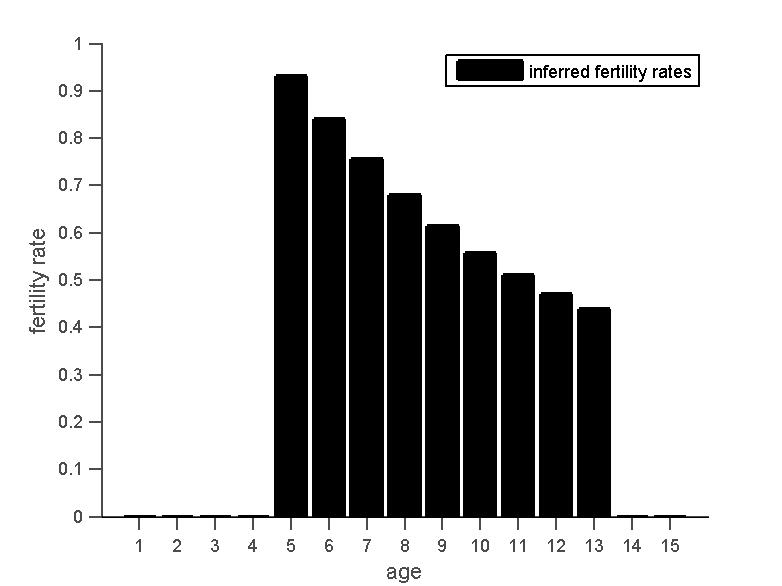
\includegraphics[scale=.22]{inferred_fert_by_age.jpg}
\caption{}%
\label{fig:fertsurvsub1}
\end{subfigure}%
\begin{subfigure}{.5\textwidth}
\centering
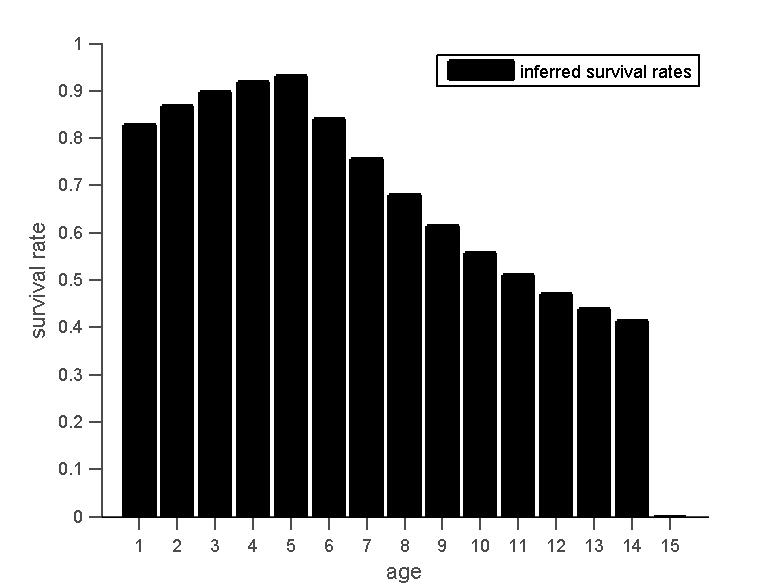
\includegraphics[scale=.22]{inferred_surv_by_age.jpg}
\caption{}
\label{fig:fertsurvsub2}
\end{subfigure}%
\caption{fertility and survival rates of Reference Leslie Matrix obtained by \emph{folding} over \emph{parity} and \emph{heterogeneity} of an (\emph{age,parity,heterogeneity})-model with one genotype with zero-parity fertility and survival rates of 0.95, and a second genotype with zero-parity fertility and survival rates of 0.55. Mutation rate $\mu$ is 0.3, maximum age $\omega=15$ age-at-maturity $\alpha=5$ and last reproductive age $\beta=13$  }
\label{fig:fertsurv}
\end{figure}%


\subsection{Effects of \PCoR\ on \vLRO\ and effective size} %% 2.2  cor affect RS in particular ind COR reduce var (COR)
\label{sec:eff_on_eff_size}
In the previous section, we have studied the effects of \PCoR\ on vital rates. However, the stochastic realizations of these vital rates, as they combine with the fertility-\emph{parity} trade-off, also have repercussions on fitness, and in particular its variance. This fitness variance can either be measured by the exact calculation of the variance in lifetime reproductive success \vLRO\, or by demographic variance \vd\, the infinitesimal variance of individual contributions to growth rate. %%effect of individual stochasticity on stochastic growth rate :the demographic variance.\\
 These two measures are projections in the dimension of individual variance, of the two main fitness measures \Rzero and \lam\ and often correspond to different research areas.  
In appendix section \ref{sec:demvarandLROvar} section we try and reconcile these two concepts in the case of age-structured populations, and disclose  their equivalence for stationary populations.In this section, we shall focus on \vLRO\ as it was, until the recent advent of stochastic growth rate studies, the key measure of individual variance in evolutionary demography, and in particular with respect to its evolutionary consequences on effective population size.\\

Investigating the impact of the costs on the variance of \LRO only makes sense if the effect on the expectancy of that quantity - \Rzero - is known. In other words, if we know $\mathbf{R_{0}}\left[\mathbf{M^{fold}_{age}}\right]$, $\mathbf{R_{0}}\left[\mathbf{M^{fold}_{age,parity}}\right]$ and $\mathbf{R_{0}}\left[\mathbf{M^{fold}_{age,strategy}}\right]$ as functions of $\mathbf{R_{0}}\left[\mathbf{M}\right]$. Because, by construction \lam\ is preserved by \emph{folding}, this step is not necessary when investigating \vd\, but necessary for \vLRO. Intuitively we expect \Rzero\ to be preserved by \emph{folding}. This is however, in general, not the case (see appendix \ref{sec:R0notpres}). However we show, in appendix \ref{sec:preseveRzero}, that, for multitrait models implementing \emph{age}, \emph{folding} over other traits than \emph{age} does preserve the net reproductive rate, thus encompassing, in the evolutionary neutral framework of the \emph{Trait Level Analysis}, both \lam\ and \Rzero. As $\mathbf{R_{0}}\left[\mathbf{M^{fold}_{age}}\right]=\mathbf{R_{0}}\left[\mathbf{M^{fold}_{age,parity}}\right]=\mathbf{R_{0}}\left[\mathbf{M^{fold}_{age,strategy}}\right]=\mathbf{R_{0}}\left[\mathbf{M}\right]$, we now focus on the study of the effects of the costs on \vLRO.

%% to asymptotical-equivalent   In other words, This will not be necessa  

  
%% Whatever the measure used, the effect of \PCoR on fitness variance impacts effective population size, which in turn has several evolutionary consequences.\\

\subsubsection{\emph{Individual components} of costs of reproduction lessen \vLRO}  
\label{ahahah}
%%We have just analyzed the buffering effect of \PCoR\ with respect to the deterministic mean vital rates at the population level (in previous section \ref{sec:eff_on_sec_grads}). We have already observed that this buffering effect is also at work at the level of each individual when comparing the distribution of time spent in the different parity classes between (i) the full (\emph{age-parity})-model implementing the costs and (ii) the \emph{folded} ergodic-equivalent model $\mathbf{M^{fold}_{parity}}=\mathbf{M^{*}}$ in which they are absent % can be seen in the different distribution of parity trajectories (calculated from the fundamental matrix $\mathbf{N}$ and plotted in figure 
%%(figure \ref{fig:comptimespentparities} page \pageref{fig:comptimespentparities}). 

In this section, we will focus on the distribution of \LRO\ between models implementing the \PCoR and asymptotically-equivalent matrices from which they are absent/ %%at age-at-death, i.e. on the lifetime reproductive output \LRO. 
In particular, we will aim our attention at the second moment of this distribution, \vLRO, in order to bring to light the patterns of the effects of the \PCoR\ on individual trajectories. \\

In appendix section \ref{blalalalalala}, we formally demonstrate (eq. \ref{eq:demons}) that costs of reproduction reduce \vLRO. Indeed we show that $ \sigma^{2}_{\mathcal{LRS}}\left[ \mathbf{M}\right] -\sigma^{2}_{\mathcal{LRS}}\left[ \mathbf{M^{*}}\right] \leq 0$, by focusing on the parity distributions, at stable-state, in the successive age-classes in both models. 
%%If \M's transitions are known, this result can be easier obtained by using the sensitivity matrix-based calculations of the demographic variance (when given a specific model, see supplementary material section \ref{sec:demvarcalc}) and the \vd\ / \vLRO\ equivalence (see appendix section \ref{sec:demvar_vs_LRO}). \\
 
%% With this equivalence in mind, the easiest way to confirm the intuition that costs of reproduction lower the variance in reproductive output, is however, simply, to consider the general formula of \vd\ (equation \ref{eq:sigmad}, p.\pageref{eq:sigmad}) for both \M\ and $\mathbf{M^{*}}$, but in a way where \M\ is only characterized by \emph{age}. In other words, this means, that instead of using the general MPPM framework, where in the full model $\lbrace \mathbf{M},\mathbf{s}, \mathcal{F},\mathcal{S}\rbrace$ where all traits are incorporated in \M, and thus the stochastic processes for different states are independent (which allowed to simply equation \ref{eq:sigmad}, p.\pageref{eq:sigmad}, into equation \ref{eq:demgvar}, p.\pageref{eq:demgvar}), the complexity of the other traits than age is tranfered from the matrix to the stochastic processes. In that framework, by properties of \TLA, $\mathbf{M}=\mathbf{M^{*}}$.  By applying eq. \ref{eq:sigmad} to \M, and eq. \ref{eq:demgvar} tp $\mathbf{M^{*}}$, we get :
%%\[
%% \sigma_\mathrm{d}^2\left[ \mathbf{M}\right]- \sigma_\mathrm{d}^2\left[ \mathbf{M^{*}}\right] \approx \lambda^{-2}.N. \sum_{a_{1} < a_{2}}\frac{\partial \lambda}{\partial \mathrm{M}_{1,a_{1}}}\sum_{l=\lbrace 1,a_{2}+1\rbrace} \frac{\partial \lambda}{\partial \mathrm{M}_{l,a_{2}}}.\mathrm{Cov_d}(\mathrm{M}_{1,a_{1}},\mathrm{M}_{l,a_{2}}) 
%%\]
%% As the realization of fertility at age $a_{1}$ decreases the probability to reproduce ($\mathrm{M}_{1,a_{2}}$) and survive ($\mathrm{M}_{a_{2}+1,a_{2}}$) at age $a_{2}>a_{1}$ (as it increases $p$, in both thf $f(a,p)$ and $s(a,p)$ formulas, see section \ref{sec:PCoR}), we get :  
%%$ \sigma_\mathrm{d}^2\left[ \mathbf{M}\right]- \sigma_\mathrm{d}^2\left[ \mathbf{M^{*}}\right] <0$. 
And therefore, the \PCoR\ buffers individual stochasticity.\\

To better understand the effects of the \PCoR\ on \vLRO\, we plot in figure  \ref{fig:varreprosuccess}, for a range of zero-parity fertility and survival rates (and maximum age $\omega=5$), the difference in variance for a \emph{constructed} (\emph{age}-\emph{parity})-matrix $\mathbf{M2}$ with the \PCoR\ and its \emph{folded} Reference Leslie Matrix ($\mathbf{M2^{*}}=\mathbf{M2^{fold}_{age}}$) without the costs. Figure  \ref{fig:diffvar} depicts the difference in variance - $ 
 \sigma^{2}_{\mathcal{LRS}}\left[ \mathbf{M2}\right] -\sigma^{2}_{\mathcal{LRS}}\left[ \mathbf{M2^{*}}\right]$ - and figure \ref{fig:diffcoefvar} the difference in coefficient of variation, $ 
\frac{\sqrt{\sigma^{2}_{\mathcal{LRS}}} }{\mathbf{R_{0}}}\left[ \mathbf{M2}\right] -\frac{\sqrt{\sigma^{2}_{\mathcal{LRS}}} }{\mathbf{R_{0}}}\left[ \mathbf{M2^{*}}\right]$. For reference, we also plot the $\sigma^{2}_{\mathcal{LRS}}\left[ \mathbf{M^{*}}\right]$ in fig. \ref{fig:varnocor} and the iso-fitness curves (for both \lam\ and \Rzero) on the zero-parity rates map (fig \ref{fig:lamminusrzero}).\\

\begin{figure}[htbp]%[hbtp]
\centering

\begin{subfigure}{.5\textwidth}
\centering
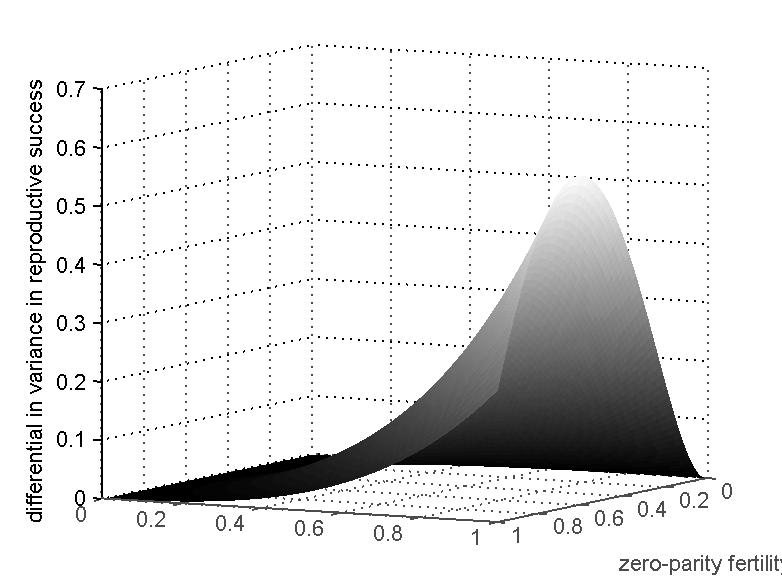
\includegraphics[scale=.22]{diffVarCoR.jpg}
\caption{}
\label{fig:diffvar}
\end{subfigure}%
\begin{subfigure}{.5\textwidth}
\centering
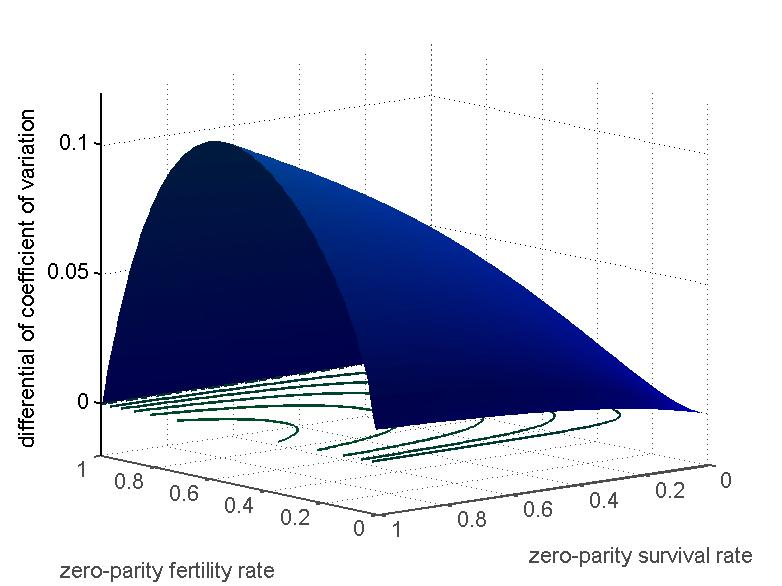
\includegraphics[scale=.22]{coeffvariationdiff.jpg}
\caption{}
\label{fig:diffcoefvar}
\end{subfigure}
\\
\begin{subfigure}{.5\textwidth}
\centering
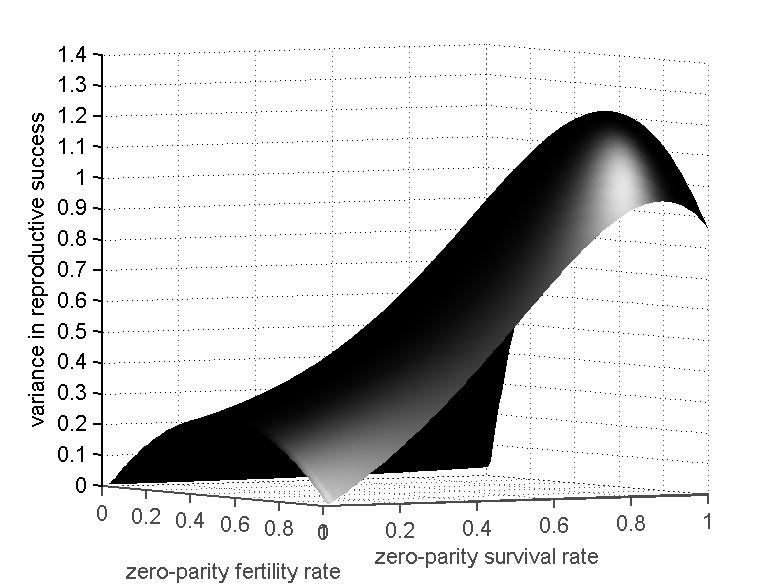
\includegraphics[scale=.22]{Varnocor.jpg}
\caption{}
\label{fig:varnocor}
\end{subfigure}%
\begin{subfigure}{.5\textwidth}
\centering
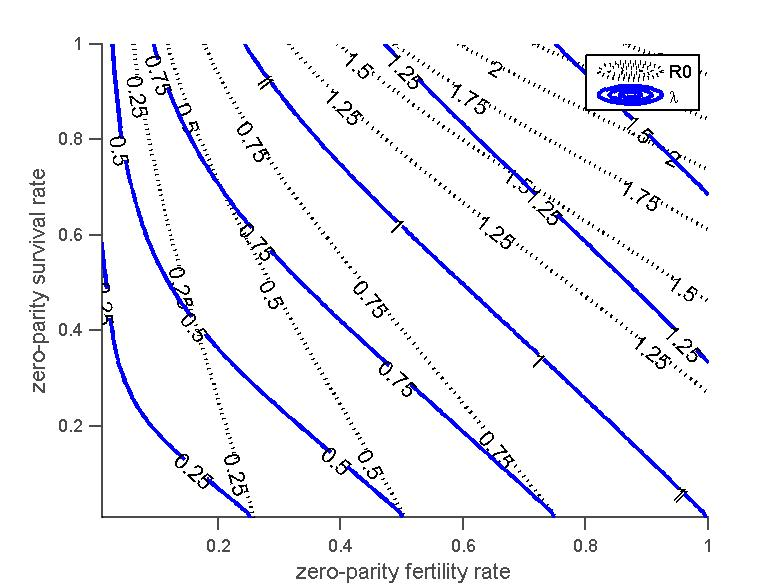
\includegraphics[scale=.22]{lamR03.jpg}
\caption{}
\label{fig:lamminusrzero}
\end{subfigure}

\caption{ For (\emph{age}-\emph{parity})-multitrait matrices implementing the \PCoR\ (differing only in their zero-parity vital rates) and their related \emph{folded} Reference Leslie Matrices from which they are absent, the difference in variance \ref{fig:diffvar}  and coefficient of variation  \ref{fig:diffcoefvar} of lifetime reproductive success between the model. The variance in lifetime reproductive success for the Reference Leslie Matrix is also displayed fig. \ref{fig:varnocor}. The value of fitness measures, \Rzero  and $\lambda$ are represented for each combination of zero-parity vital rates  on fig \ref{fig:lamminusrzero}. The population has maximum age $\omega=5$ and age-at-maturity $\alpha=1$. As per the generic model in this article, the \PCoR\ is modeled by relatively decreasing each vital rate by $\sfrac{1}{(1+\omega -\alpha)}$ per parity.}
\label{fig:varreprosuccess}
\end{figure}



The first observation, is that the costs reduce variance (fig.\ref{fig:diffvar})  and coefficient of variation (fig. \ref{fig:diffcoefvar}) of \LRO. The first, we have discussed above and formally demonstrated in appendix \ref{blalalalalala}. The second ensues from the first, as \Rzero\ is preserved by folding in such models (see section \ref{sec:preseveRzero}). The second observation, is that the effects of the costs on \vLRO\ (fig.\ref{fig:diffvar}) follow the general shape of \vLRO\ itself (fig. \ref{fig:varnocor}), at which we shall now take a closer look. \\

The shape of \vLRO\ as a function of zero-parity rates $f$ and $s$ ( eq. \ref{eq:varLRO}) - reveals that it results from the combined effects of three parameters. First, the variance in fertility rates at each age, $Var(\mathcal{F^{*}}_{a})=f^{*}_{a}(1-f^{*}_{a})$ , which is the engine of the variance in \LRO\ and confers to the latter, the $x(1-x)$ shape of the former, along the zero-parity fertility rate axis. The importance of $Var(\mathcal{F^{*}}_{a})$ for late ages however requires survival ($P_{i}$ in eq. \ref{eq:varLRO}), and thus the increase in \vLRO\ as survival increases. At the same time, as age increases, on average $f^{*}_{a}$ decreases because of the costs. Therefore even very high zero-parity fertility rates (conferring no variance in $\mathcal{F}_{a}$ at early ages) will at late ages generate variance. Hence, the asymmetrical $x(1-x)$ shape at high survival rates, across fertility rates. Finally, survival does not only act as a promoter of variance in fertility, but as a stochastic process itself - $s_{i}(1-s_{i})$ in eq. \ref{eq:varLRO} - which explains the decrease in variance as survival reaches its maximum levels. These last two effects, explain why in this model, the maximum \vLRO\ is reached by organisms with zero-parity (survival, fertility) coordinates of $(s=0.94,f=0.64)$.\todo{preciser que l on veut dire par la que survie n est pas a 1 et fertilité decentralisée ?}\\

This general shape - the $x(1-x)$ pattern on zero-parity fertility axis and general increase with survival- is preserved when switching from \vLRO\ (fig.\ref{fig:varnocor}) to  $\sigma^{2}_{\mathcal{LRS}}\left[ \mathbf{M}\right] -\sigma^{2}_{\mathcal{LRS}}\left[ \mathbf{M^{*}}\right]$ \todo{mettre un delta ?}(fig.\ref{fig:diffvar}). This is due to the difference being a linear function of variance itself, as shown in equation \ref{eq:vardiff} (appendix \ref{blalalalalala} page \ref{eq:vardiff}). However this equation also shows the difference in variance to also linearly depend on survival and fertility. This explains why the difference in variance between models with and without the costs (fig.\ref{fig:diffvar}) increases with survival even at high survival rates, and is flat at very low survival rates. These patterns are preserved when correcting for \Rzero, i.e. for high fertility and survival rates, as can be observed from the differential in the coefficient of variation (fig.\ref{fig:diffcoefvar}). Logically both the exponential increase with survival and the the asymmetrical effect for high fertilities disappear. These observations demonstrate that even though very short-lived or semelparous organisms (i.e., with $s \approx 0$) exhibit variance in reproductive success (fig \ref{fig:varnocor}), the costs of reproduction does not affect it (figs \ref{fig:diffvar} and (fig \ref{fig:diffcoefvar})) and that the effects of the costs will increase with iteroparity/longevity.\\



%%With regards to the difference in variances, the effect of survival on longevity, and of longevity on the efficiency of the buffering effect of costs of reproduction, implies that variance difference is more linearly dependent to zero-parity survival rate, whilst keeping a $x(1-x)$ shape on the fertility axis. And so , variance differential  is completely flat when survival is at 0, and maximum when survival is at 1. (see equation \ref{eq:vardiff} for formal proof). 
%%
%%The first ones are semelparous organisms and costs of reproduction have not effect on them, the second ones at long-lived organisms with plasticity in the fertility trajectories and thus maximum buffering effect  \\
%%For organisms with high zero-parity survival rate (fig. \ref{fig:varnocor})  the $x(1-x)$ shape of the across fertility rates curves for high survival rates is actually asymmetrical for variances and then their difference. That is due to the fact that a very high fertility rate is only very high for zero-parity, and for such long lived organism with very high fertility rates at maturity, costs of reproduction will progressively reduce the mean fertility rate to levels at which variations between individuals will occur. 
%%To correct for that effect, we also provide the difference in coefficient of variation ((fig. \ref{fig:diffcoefvar})\\
%%


%%And thus we the same $x(1-x)$ shape curve when crossing along the fertility axis than in the variance itself (fig. \ref{fig:varnocor}) and typical of variance of Bernoulli processes. However the shape of the variances and of the difference in variances differ with regards to the effect of survival. \\
%%Survival via its effect on longevity is the fuel of variance and thus of their difference (see equation \ref{eq:vardiff}), with higher values at high survival rates.\\


\paragraph{Iso-fitness combinations of vital rates} From an evolutionary life history perspective however, considering organisms with very different fitness (the iso fitness curves for \Rzero\ and \lam\ are represented on figure \ref{fig:lamminusrzero}) does not make a lot of sense. 
Therefore, from the statistics plotted in figure \ref{fig:varreprosuccess} for all possible zero-parity vital rates, we can extract the combinations that are iso-fitness, i.e. that only differ in strategy. In figure \ref{fig:diffvarlam1}\todo{legende a normaliser !}, we represent, for each possible zero-parity fertility rate, the corresponding zero-parity survival rate for a fitness of $\lambda \approx \mathbf{R_{0}}\approx 1$ (grey curve, right y-axis). For each such pair of coordinates, we extract the variances in \LRO\ for each model (blue curves, left y-axis), and their difference (red curve, left y-axis).
%% From the data gathered it is possible to focus on specific iso-fitness trajectories, which zero-parity vital rates correspondences are depicted in figure \ref{fig:lamminusrzero}.
This clarifies the general conclusions drawn above for the particular case of organisms that are iso-fitness (here all organisms have stationary growth rate, and therefore \Rzero\ worth unity): the variance in reproductive success requires both variance in fertility and survival and is therefore maximal for intermediary values of $f$ and $s$, but survival is also required to promote late fertility, and this pushes $s_{max}$ higher and therefore $f_{max}$ lower than the point of equal coordinates ($f=0.54$, $s=0.54$). 
As expected, because of the costs of reproduction, this is less true for $\mathbf{M2}$, for which $s_{max}$ is lower and therefore $f_{max}$ higher than for $\mathbf{M2^{*}}$. To the contrary, the differential in variances between the two models (red curve), is maximal for the maximum possible survival rate $s=1$ and its related zero-parity fertility-rate $f\approx 0.22$. In other words, this result shows that whilst the effect of individual stochasticity is not a monotonous function of the pace of organisms as measured by their position on the slow-fast continuum \citep{Gaillard1989,Stearns1983} , the \emph{effects} of costs of reproduction on such individual stochasticity increase with pace and are maximum for slow organisms.\\


  
%%  We have specifically extracted all pairs of vital rates yielding a stationary population and plotted both variance and their difference in figure \ref{fig:diffvarlam1}. here again, we can see that the highest difference in variance corresponds to the highest survival /lowest fertility rate combination, that is the longest generation time (to buffer reproductive success) whereas variances themselves are higher at intermediate levels for zero-parity vital rates.




\begin{figure}[hbtp]%[hbtp]
\centering
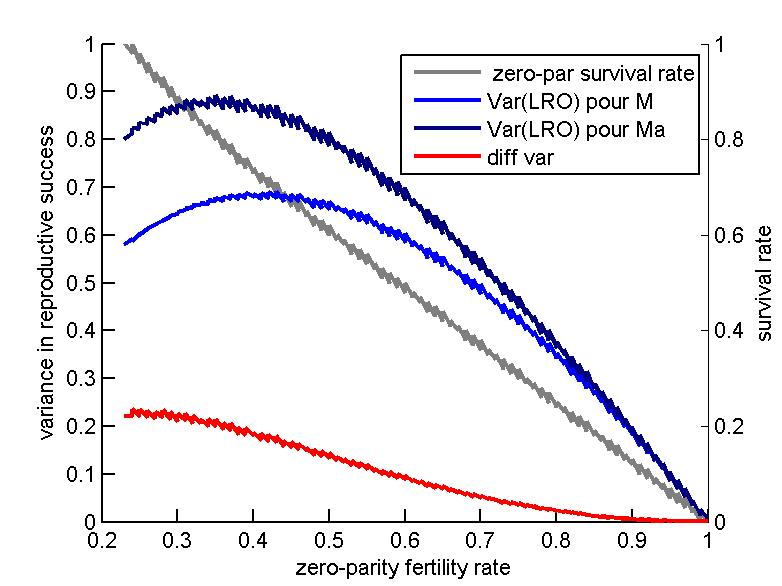
\includegraphics[scale=.22]{diffvarlam1.jpg}

\caption{ For all combinations of zero-parity vital rates yielding an ergodic growth rate $1-\epsilon \leq \lambda \leq 1+\epsilon$ (with $\epsilon=0.01$),for each zero-parity fertility rate, the related zero-parity survival rate, and the variance of reproductive output for the model (implementing \PCoR) and its reference leslie model with no trade-off implemented and their difference;The population has maximum age $\omega=5$ and age-at-maturity $\alpha=1$. Cost of reproduction is modeled by relatively decreasing each vital rate by $\sfrac{1}{(1+\omega -\alpha)}$ per parity.}
\label{fig:diffvarlam1}
\end{figure}

\paragraph{Adding heterogeneity into the mix ...} 
 ... raises questions with regard to the cross-effects of the costs and heterogeneity on the variance in reproductive success of the overall population and of the relative importance of heterogeneity and stochasticity as components of \vLRO\ for populations with and without the \PCoR. In appendix \ref{sec:heterovlro}, we demonstrate that costs of reproduction and heterogeneity act independently on \vLRO\ and in particular that the heterogeneity component of the variance in lifetime reproductive success %(equation \ref{eq:hetvarLRO} page \pageref{eq:hetvarLRO})
is unaffected by costs. We also show there, that the \PCoR increase the relative importance of the \emph{fixed} (aka \emph{adaptive}) heterogeneity component of \vLRO\ as it remains constant whilst the effects of individual stochasticity on the \emph{dynamic} (aka \emph{neutral}) component of heterogeneity is reduced. However, it still remains low with comparison to the principal generator of demographic variance: individual stochasticity \citep[in agreement with many authors, see for instance][]{Snyder2018,Steiner2012}.



\subsubsection{Demographic variance and effective size}
\label{sec:demvareffsize} 
%%\todo{ici calcul sensi (pour pouvoir mult par N) alors qu'avant elasti (pour raison multiplicatinve) ... on peut homogeneiser ?}
 In the field of population genetics, the effective size, $N_{\mathrm{e}}$, corresponds to the size of an 'ideal' population yielding the same rate of genetic drift \citep{Wright1931} than the 'real' population of total size $N$. The 'ideal' population of population genetics is a stationary population of diploid individuals with non-overlapping generations and where all individuals in the current generation have the same probability of being the parent of each individual in the next one.
This characteristic implies that, in the ideal population, each of the $N_{\mathrm{e}}$ adults has probability $p=\frac{1}{N_{\mathrm{e}}}$ of being parent of each of the $N_{\mathrm{e}}$ offspring. The expected \LRO\ of a parent is therefore the sum of $N_{\mathrm{e}}$ independent Bernoulli processes of parameter $p$, that is, by the Poisson paradigm, a Poisson law of parameter $\sum_{i=1}^{N_{\mathrm{e}}} p =1$. Therefore, a variance larger (respectively lower) than 1 - or, more generally for non-stationary populations, than the mean - implies conversely a non-Poisson family size, and thus a non-random distribution of parents. This implies an increase (resp. decrease) in genetic drift rate, and therefore a smaller (resp. larger) effective size $N_{\mathrm{e}}<N$ .\\

By definition, the effective size of a population thus determines the strength of genetic drift. It also determines the increase in inbreeding coefficients and the effectiveness of selection: 
the fate of an allele, of selection coefficient $s$ in a population of effective size $N_{\mathrm{e}}$, is provided by the effective selection coefficient $s.N_{\mathrm{e}}$ which combines both the effect of selection ($s$) and the effect of variance of reproductive success on genetic drift (through $N_{\mathrm{e}}$). The effect of demographic variance on effective selection has also been studied directly. First, by Gillespie \citep{Gillespie1974,Gillespie1975}, showing the selective advantage of reduced variance in offspring number; and later many others \citep[see, for instance,][]{Shpak2005,Shpak2007,Giaimo2014}.  \\

An \emph{age}-structured population model - represented matrixwise by a Leslie matrix - infringe many laws of Wrightean 'ideal' populations. The population it models is made of haploid individuals, which number of offspring is not a Poisson and which generations overlap. Moreover the growth rate of such models is allowed to deviate from the stationarity of the population genetics 'ideal' population. The effective size of such age-structured populations has been extensively studied by \citet{Felsenstein1971}, \citet{Hill1979,Hill1972} and \citet{Nomura1996a} but our study is not so much about the absolute effect of trait \emph{age} on effective size as about the relative effect of trait \emph{parity}, embedding the \PCoR, and its \emph{folding} upon, in an \emph{age}-structured population. %% is not our concern here as we merely wish to understand the relative effect between different age-structured populations with or without \PCoR.\\

\paragraph{The \PCoR\ increase $N_{\mathrm{e}}$}
The allele frequency variance - the engine of genetic drift - is, in an haploid population, $V_{p} \approx p(1-p)\sigma^{2}/N$. From this, \citet{Engen2005} demonstrates that for age-structured populations the effective size can be approximated by $N_{\mathrm{e}} = \frac{N}{\sigma_{\mathbf{d}}^{2}.T}$ where $T$ is generation time. From the correspondence between \vLRO\ and \vd\ established in appendix \ref{sec:Var_LRO and Var_d}, we can consider that \citet{Engen2005}'s result is a generalization of \citet{Hill1972}'s effective size formula for age-structured stationary populations $N_{\mathrm{e}} = \frac{N \bar{b}T}{\sigma_{\mathcal{LRS}}^{2}}$.Thus, in all cases, the reduction of demographic variance caused to the fertility buffering effect of \PCoR\ implies that these increase effective size. In other words, the $N_{\mathrm{e}}$ of an age-structured population is underestimated when the costs are not accounted for.  Compared to an asymptotically equivalent population without the \PCoR , the population with the costs is therefore less prone to genetic drift and more to selection. This is all the more important to consider when modeling age-structured populations of small sizes. 
%%This result also implies that inbreeding coefficient will increase less in the population with \PCoR. From a \emph{kinship demography} point of view, finally, this difference between the two models in variance of family sizes hints at the fact that the entire kinship distribution in the stable-state population will be vary. \\
The reducing effect of the costs on selection gradient \citep[see][]{Coste2017} now needs to be revisited in the light of their concurrent positive effect on selection effectiveness. To do that we devise the following effective selection measure, we call \emph{variance-effective selection gradient}, $\frac{1}{\sigma^{2}_{\mathcal{LRS}}}\frac{\partial \lambda}{\partial f_{a}}$, that allows to compare selection gradients between models with differing \vLRO.  As we can see in figure \ref{fig:scaledselgradbyvar}, representing the \emph{variance-effective selection gradient} for the same ergodic-equivalent models with and without for which the absolute selection gradient plotted in appendix fig. \ref{fig:selgrad1}, the reducing  effects of the costs on demographic variance does not necessarily obliterate their weakening effects on the force of selection.\\


\begin{figure}[hbtp]%[hbtp]
\centering
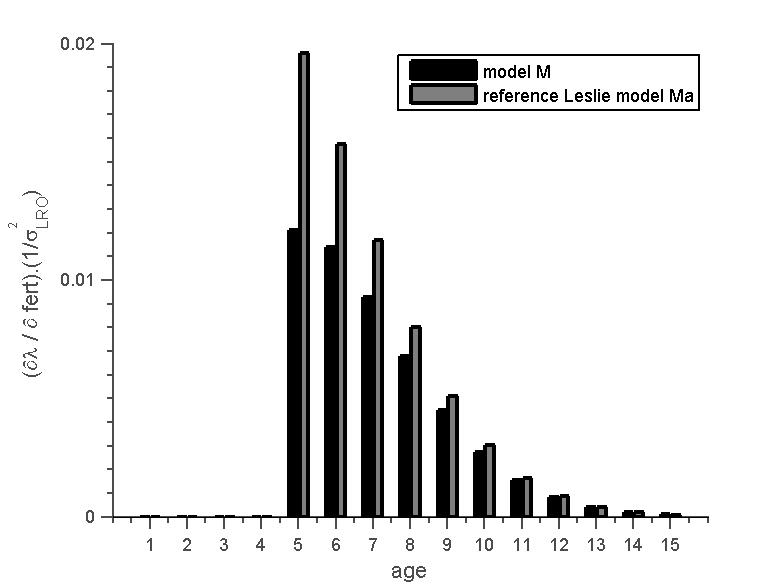
\includegraphics[scale=.25]{scaledselgradbyvar.jpg}
\caption{Effective size-scaled selection gradient  measured by the sensitivity of ergodic growth rate to fertility rates,summed by age divided by variance of reproductive success, for \M modeling an (\emph{age-parity}) population with physiological costs of reproduction and \Ma its reference Leslie matrix, which is \M folded on \emph{parity}, modeling the same population but characterized only by age. The population has maximum age $\omega=15$ and age-at-maturity $\alpha=5$. The zero-parity fertility and survival rates are 0.85. Cost of reproduction is modeled by relatively decreasing each vital rate by $\sfrac{1}{(1+\omega -\alpha)}$ per parity.}
\label{fig:scaledselgradbyvar}
\end{figure}

\paragraph{\emph{Genetic components} of the costs buffer fast organisms and \emph{individual component} buffer slow organisms }
However, as one shifts towards the slower end of the spectrum, the variance-effective selection gradient for fertility at age $a$ is less and less decreased by the \PCoR, and is actually increased by the costs for very slow organism. This is provided in appendix \ref{sec:PCORincVarEffSelGrad_of_slow_org}.
This results hints at a stabilizing role on Antagonistic Pleiotropy - i.e. on the \emph{genetic component} of the costs of reproduction- for the \PCoR. Whilst in \emph{age}-structured populations without individual costs, selection gradients  vary massively between fast organisms - with steep gradients fast inviting even faster alleles in the population - and slow ones - which almost flat gradient incline seems to prevent any AP - we see that the \PCoR\ will smooth these differences, straightening the (variance-effective) gradients of fast organisms and curving the gradients of slow ones. When accounting for the \PCoR, Antagonistic Pleiotropy on fertility seems to work at much closer rates on all organisms, fast and slow, to which, in a constant environment, it continuously provides faster alleles better suited to benefit from this constancy. Still however, variance-effective selection gradient are flatter for slow organisms : AP will be less efficient for these, as a buffer - at the \emph{species} level - of stochasticity. However, the longevity of slow species ensures that this can be compensated by the \PCoR (at the base of the Disposable Soma Theory) which buffer stochasticity at the \emph{individual} level.

 
%% There is also a Life History interpretation of the phenomenon, as it clearly appears that, if \PCoR, do, on an organism with no strong bias towards early fertility or survival, reduce the selection gradient inviting genotypes with higher early fertilities (at the cost of later fitness), in a way that seems to limit the cohabitation of \PCoR and \GCoR   , this is not the case for populations with populations biased towards early survival. And thus it seems that \PCoR, via their effects on both selection gradients and \vLRO , will be a generator of stabilizing selection towards a location on the iso-fitness early fertility/survival strategies curve that is particuliar to the current environment and life history, whereas \GCoR are the product of a directional selection, incessantly inviting genotypes with higher early fertility rates (selection gradients - when taken as sensitivities of \lam to fertility rates - are always decreasing with age). This effect of \PCoR may be one of the answers to the question of knowing why all organisms do not evolve towards semelparity (a natural expectation when only considering antagonistic pleiotropy theory and \GCoR) \\
 




\section{Discussion}
\label{sec:discussion}
%%\section{Results}

In this article, we hint at the power of \emph{Trait Level Analysis} as a tool to improve our understanding of the consequences of individual heterogeneity and in particular of its two components - \emph{fixed} and \emph{dynamic} - by focusing on their Life History Trade-Offs counterpart: the \emph{individual} and the \emph{genetic components}. Specifically we provide a matrix model for the costs of reproduction, which individual component is related to the Disposable Soma theory of senescence and genetic component to the Antagonistic Pleiotropy.
%%This chapter consists in hinting at the first answers to the questions asked in chapter 1 thanks to the MPPM framework developed in chapter II.
Analysing the 3-trait Multitrait Population Projection Matrix, allows understanding that these two components, whilst having similar phenotypic manifestations (negative correlations between vital rates at different ages for costs of reproduction, for instance) are actually very different on many levels and in particular the level of action (individual vs population) and the time window of effect (generation time vs evolutionary time). The analysis shows that they are not mutually exclusive, and therefore they can be both implemented in the same matrix models, as we do in this article. This allows to better understand their relative, cross and joint effects on the demography and evolutionary dynamics of a population. In particular, whilst it is well known that genetic trade-offs have effects at the level of the individual (physiological for instance, that promote certain functions in certain lineages in the population and not in others), it less obvious that individual trade-offs have evolutionary consequences. \emph{Trait Level Analysis} of MPPMs embedding both components of LHTOs allow to predict such consequences.
Indeed, the MPPM framework allows to implement - with the addition of \emph{dynamic} and \emph{static} traits – both components of LHTOs and permits to analyze the evolutionary demographic repercussions of these trade-offs by \emph{folding} the model on the trait incorporating it. In the particular - but essential - case of costs of reproduction, such a model therefore enables the study the cross effects of both components of costs and, above all, to measure the evolutionary consequences of the \PCoR.\\

In this article, we have devised a family of MPPMs able to model various populations differing in their position on the genetic component of the costs - i.e. differing in pace of life - but all encountering the \PCoR: the zero-parity vital rates, defining the life history  strategy of the population, is reduced as parity increases. 
%%This simple setup allows to incorporate the key elements of \PCoR\, as discussed in chapter 1, with trait \emph{parity} in the role of Ratchet Capital, and Fluctuating Capital reduced to environmental effects. 
In case of heterogeneity in the population, i.e. if different genotypes with different life-history strategies- iso-fitness or not – cohabit in the population, we show how to integrate these elements to generate an (\emph{age-parity-heterogeneity})-MPPM  that can incorporate \PCoR, \GCoR\ and heterogeneity in fitness in the population. Then, we provide new tools to yield the key fitness measures of a population structured by several categories. In particular, we provide formulae for \Rzero and its variance for models with fixed heterogeneity and/or dynamic heterogeneity. 
We have then combined fitness measures computation tools with the properties of the \emph{Trait Level Analysis} - that allows to \emph{fold} a model implementing the \PCoR over \emph{parity} to generate an asymptotic-equivalent model from which the costs are absent - to measure the demographic and evolutionary effects of \PCoR. First, by extracting the vital rates from the Reference Leslie Matrix of an (\emph{age-parity-heterogeneity})-MPPM, we show the mechanical role played by both components of costs on the shape of mortality and fertility curves represented by \emph{age} only.
%%Second, we show that the \PCoR\ reduce the fertility selection gradient. This result highlights the buffering effect of the costs on fertility stochasticity (described in chapter 1) whereby the increase of realization probability of a particular fertility event would have limited positive effect on \lam\. Indeed, it would set individuals on higher parity trajectories with therefore reduced future vital rates. By considering the selection gradients of the matrices folded on \emph{parity}, \emph{heterogeneity} and both, we can extend the results from \citet{VanNoordwijk1986} and \citet{Houle1991} and show that the variance in allocation strategy itself might prevent detectability of the allocative costs. \\ 
%%Surprisingly, the overall decrease in selection gradients caused by \PCoR, seems to imply, contrary to our expectations from chapter 1, that physiological and genetic costs might not cohabit in organisms. Physiological costs, if present, would flatten the selection gradient, preventing the invasion of different life-history strategies in the population, whilst if absent the steep curve of the gradients would, according to \citet{Williams1957}’s antagonistic pleiotropy theory, invite faster alleles in the population. \\
Second, we have analyzed the reducing effects of the \PCoR\ on the variance in lifetime reproductive success. We show moreover that this effect is stronger for long-lived organisms, for which, even along an iso-fitness continuum, the decrease in variance caused by the costs is maximal. Via the role played by the variance in reproductive success on the effective size of a population, this results has important consequences on efficient selection. This prompts us to revisit the results stemming from the calculation of the absolute selection gradient and introduce the \emph{variance-effective-selection gradient} that scales the absolute selection gradient by the inverse of \vLRO. When considering this efficient selection measure, we realize that, whilst the net effect of the costs is still a reduction, for very slow organisms the \emph{variance-effective-selection gradient} is increased by the \PCoR. This hints at the fact that the seemingly very large differences in gradients between short (very steep gradients) and long-lived (much flatter gradients) organism, when structured and analysed by \emph{age} (only), with its corollary exponential invasion of faster alleles for already fast organisms, may be an artifact of models forsaking the implementation of trade-offs. \\

%%In the following section, we consider another measure that, like the  \emph{variance-effective-selection gradient}, combines both the deterministic and the stochastic effects of the costs: the stochastic growth rate. We know that \TLA\ preserves \lam. We showed that costs reduce \vLRO\, it therefore reduces demographic variance by their equivalency (appendix \ref{Var_LRO and Var_d}). In that section, by formally proving that \PCoR\ also buffer environmental variance, we establish that they, in all cases, increase the stochastic growth rate. To illustrate this, we have simulated the fate of populations modelled by the two ergodic-equivalent matrices with and without the costs, in the same environments. The effect of the costs on environmental variance can be observed by comparing the populations between the two models. The effect of the costs on demographic variance can be seen by comparing the variance in trajectories within the populations (sharing the exact same mean parameters) of the same model. The combination of both effects provides a better resilience to the model with \PCoR.\\

This relatively simple MPPM model therefore yields several important results, in the light of senescence theories. It highlights the general buffering effects of the \PCoR (at the core of the Disposable Soma Theory) on the variance in reproductive success. Moreover it also shows that the allocation process at the core of DST is not the only mechanism able to buffer life-history: 
%%The sheer longevity of certain organisms, and by then the spreading of their reproductive schedule, already reduces the importance of single fertility events. 
the \emph{genetic component} of the costs (related to the Antagonistic Pleiotropy theory) buffer organisms, at the population level, over evolutionary times against stochasticity whilst the \emph{individual component} of the costs (related to the DST) buffer organisms, at the individual level, at the time scale of the generation time, against individual stochasticity.\\
 
%%And therefore the Disposable Soma theory seems to act as a regulator of the strength of the Antagonistic Pleiotropy theory, which, in turn, may hint at a combined role in inviting and filtering the variance in life history strategies in a population.\\

From a methodological point of view, this article also highlights the strong limitation of life-history models structured by \emph{age} (only). It is often argued that these models are ideal to study populations for which age is the main determinant of life history. However this paradigm, we have shown here, has to be moved beyond. First because trade-offs are a key component of life history and that, to be implemented, a trade-off needs at least two traits to lean on. Second, because age is only the best predictor of vital rates as it already encompasses some consequences of the Life History trade-offs. We showed how a model where vital rates do not depend on age, can seem to be strongly age-driven when \emph{folded} upon the costs of reproduction. Whilst using only one trait, partially incorporating, by linkage the underlying trade-offs (and thus seemingly life history determinant) will generally provide appropriate results with respect to population dynamics and demography, it will generate poor analyses from an evolutionary demography viewpoint. This can be readily ascertained by any empiricist when comparing the variance in reproductive success inferred by the Leslie Matrix generated by the Life History Table of her/his studied organism with the actual statistics from the field. We show, in this article, that this discrepancy is only one in many consequences of interpreting \emph{age}(only)-structured models without understanding the effects of the simplification.
It could therefore be argued that the addition of a 2nd trait on an age-structured model is as key to understand the life history of an organism from an evolutionary perspective, than the addition of the 1st trait (e.g. \emph{age} or \emph{stage}) - compared to a non-overlapping generation model - was from a demographic viewpoint. In general, this prompts us to revisit general results stemming from one trait analyses. For instance, \Citet{Charlesworth1980} demonstrated that the \emph{age}-structure of population has little impact on their population genetics. Would that result hold when a 2nd trait, implementing a constraint such as the \PCoR, is added to the age-structured model ? \\

%%In this chapter, we implement key elements of costs of reproduction as identified in chapter 1. However, for simplicity, many specific components, the combination of which make up the vast diversity of costs of reproduction in nature, were left aside. This is the case, for instance of the storage capacity, $stor$, which positions organisms on the income-capital breeding continuum according to their ability to save some of the resources they acquire from the environment (forsaking $stor$ in our model, allows to implement FC from the environmental matrices directly). This the case also of the reproductive effort schedule $res$ which represent the time distribution of effort required to produce an independent offspring. In the model of this chapter, we equate reproductive effort and fertility event. However, in most organisms, reproductive efforts start before birth (e.g., mating, gestation) and continue after (e.g., lactation). Post-natal care can be protracted, especially in social species where it takes the name of parental care. We hinted, in chapter 1 (section \ref{sec:phycodynhet} page \pageref{sec:phycodynhet}), at a way to implement an extended reproductive effort schedule in general, and parental care in particular, by adding extra \emph{dynamic heterogeneity} traits to the model trait structure. These “buckets” would segment the reproductive effort schedule, and only when the last “bucket” is filled would a new independent offspring be deemed to appear in the population. Further extending parental care to kinship care is a natural step. When an adult male human takes time and spends money to care for his grand-children, his nephew or his pregnant sister, he can be considered to be promoting the future reproductive value of his genotype, at the cost of current reproduction. Stretching \citet{Williams1966}’s definition of the costs of reproduction to include kinship care may be frowned upon, but the analogy of principles implies an analogy in potential models that we shall evoke in the next chapter. \\
%%Whilst it seems that kinship may be added as an input to the evolutionary model framework of MPPMs, section \ref{sec:eff_on_eff_size} shows us that it is an (overlooked) output of any structured model. We showed here the effect of the costs on variance of reproductive success, or family size as \citet{Hill1972} calls it, but the kinship consequences of the structure of a population extend far beyond that measure to include all distributions of kin. The combined study of the kinship input and output of structured populations, we call kinship demography, will be the topic of the next short chapter. 
%%\newpage

\section{Appendices}

\subsection{Classical classification of LHTOs}
\label{sec:app_ClassLHTOs}
The classical classification of trade-offs is field based and segregated into 'non-evolutionary' trade-offs - themselves split as internal or physiological trade-offs  (when the trade-off stems  from a constraint internal to the organism, for instance generated by y-shaped allocation mechanism because of finite resources) and external or ecological LHTOs (when the constraint is caused by the environment) – and 'evolutionary' or 'genetic' trade-offs that correspond to a constraint generated at the genotypic level (using \citet{Stearns1989b}'s genotypic level- intermediate structure-phenotypic level  classical representation of LHTOs). This classification is however not absolutely segregating, and not additive: It is indeed easy to find example s of physiological trade-offs that are also genetic. Actually most of the early evolutionary demography studies  of the 70s are about genetic  trade-offs where genes act on the allocation of resources towards reproduction or survival and hence are also physiological trade-offs.

\subsection{Growth rate sensitivities and selection gradients in models embedding hidden heterogeneity}
\label{sec:selgradsensi}
Matrix models are models of choice for evolutionary demography as they allow, among other tools, to generate \emph{selection gradients} quantifying the force of selection on a particular life-history trait embedded in the model.
Implementing \emph{hidden heterogeneity} as a family of traits, implies to input the fertility transitions between adults of a certain genotype and offspring of another and therefore to make assumptions about heredity/mutation.\\
 
In quantitative genetics models from which selection gradients stem, however, heredity and force of selection are components of the two different components which product yields the response to selection. In heritability and selection differentials in the Breeder's equation \citep{Lush1937}. In $\mathbf{G}$ (the additive genetic variance/covariance matrix) and the selection gradients in Lande's equation \citep{Lande1982}.
In consequence, in a multigenotypic matrix model, the equation between sensitivity of population growth rate to vital rates of any genotype and selection gradient has to be treated with care. The inadequacy of such a model with quantitative genetics is not surprising since the latter is about quantitative traits described with by their variances, whilst the former incorporates, from the outset, all possible (discretized) genetic variant.  %%In a model where varying genotypes are modeled as an additional trait, there is no possible additive genetic variance for each vital rate, at it corresponds to a given genotype; instead ,genetic variance would be represented with the incorporation of additional genotypes differing in their vital rates, i.e in additional elements in $\mathcal{G}$. 
The selection gradients, in such a model, then have to be calculated genotype by genotype, i.e. if $\mathcal{B}=\lbrace age\rbrace$, Leslie matrix by Leslie matrix, and not as the sensitivity of the MPPM growth rate to matrix entries. These sensitivities then can be interpreted as selection gradients of the specific genotype's vital rates. The Lande’s equation would then provide the expected change in these vital rates in a range allowed by $\mathbf{G}$ and paced by the selection gradient. If need be, new genotypes may then have to be added to $\mathcal{G}$. %%the genetic variance is still large for genotypes  This would materialize as new genotypes
%%And thus sensitivities of fitness to matrix entries can only be interpreted as selection gradients when \emph{hidden heterogeneity} is not a specific trait, i.e. by \emph{folding} $\mathbf{M}$ over $\mathcal{G}$.
In multitrait models incorporating $\mathcal{G}$ as a family of traits, because of the possible confusion between the implemented genetic variance, and the $\mathbf{G}$ matrix, we think it preferable to not refer to sensitivities as selection gradient but simply as growth rate sensitivities of matrix entries.

\subsection{Note on matrix Ma,p: vital rates,  R0 and interpretation}
\label{sec:Map}

Matrix $\mathbf{M_{a,p}}$ is matrix $\mathbf{M}$, the \textit{age-parity-heterogeneity} MPPM, \textit{folded} over \textit{heterogeneity}.  In $\mathbf{M_{a,p}}$, heterogeneity is not implemented as a trait any more, but since it was implemented in the full-traited matrix  $\mathbf{M}$ from which it is derived, it has effects on $\mathbf{M_{a,p}}$, making its interpretation both challenging and interesting.

\subsubsection*{Discrepancies in calculation of \texorpdfstring{$\mathbf{R_{0}}$}{R0}}

 In $\mathbf{M}$, because of the implementation of \PCoR\ via trait \emph{parity}, survival transitions output states depend from fertility.  Simply put, survival transitions from any state $i=(a,p,h)$ to either $j_1=(a+1,p,h)$ or $j_2=(a+1,p+1,h)$ are $\mathrm{M}_{j_{1},i}=s_{i}*(1-f_{i})$ and $\mathrm{M}_{j_{2},i}=s_{i}*f_{i}$, with a 3rd, implicit transition towards $death$ worth $\mathrm{\tilde{M}}_{death,i}=1-s_{i}$. These three transitions sum to 1.
In the MCwR tool, the corresponding fertility rewards expectations for these three transitions (in $\mathbf{Rw^{1}}$) are respectively 0, 1 and $f_{i}$. Thus the mean expected reward is $0. (s_{i}.(1-f_{i}))+1.(s_{i}.f_{i})+f_{i}.(1-s_{i})=f_{i}$  and therefore both MCwR and $\mathbf{R}$ approaches ($\mathbf{e}_{\mathcal{LRS}}=\mathbf{1}'.\mathbf{R^{*}}$, see box p.\pageref{box:noteonR0}) provide the same results for $E(\mathcal{LRS})$.
%%in \emph{expectancy}.  
%% \mathbf{R=F.N}$ 
In $\mathbf{M}_a$, the Leslie reference matrix, survival and fertility transitions are completely separated, with only one output per survival transition. Thus in this case also, both MCwR and $\mathbf{R}$ provide the same results.\\

However for the intermediary matrix, $\mathbf{M}_{a,p}$ - \M\ \emph{folded} on \emph{heterogeneity}- both measures differ. Indeed, through \emph{folding}, the survival transitions  from state $i=(a,p)$ towards either $j_1=(a+1,p)$ or $j_2=(a+1,p+1)$ will, in general, not be distributed according to the transition value between $i$ and the (unique) offspring state $1$ which we interpret as fertility rate ($\mathrm{M}_{1,i\leftrightarrow (a,p)}=f_{i}$). This is caused by the \emph{heterogeneity} modeled in \M\ expressing itself through EFP-\emph{merged} vital rates, now that \emph{heterogeneity} is not a trait any more \citep[see][]{Coste2017}.\\

Let us illustrate this, seemingly paradoxical, situation with a simple example : Let us imagine a population structured by 2 \emph{age} - and therefore 2 \emph{parity} classes - and 2 \emph{heterogeneity} classes (A and B) produced in equal measures ($m=0.5$) at each fertility event. A individuals have all vital rates at $1$ and B individuals at $0.5$.
Then all A newborns (half the population of newborns), will produce 1 offspring and become individuals of age 2 and parity 1. Half of B newborns will produce 1 offspring and half of B individuals will survive. Those halves are independent, and thus a quarter of B individuals will survive \emph{and} become adults of \emph{parity} 1, and another quarter will become adults of \emph{parity} 0.
Thus for the population \emph{folded} on \emph{heterogeneity}, i.e. where individuals are only characterized by \emph{age} and \emph{parity}, the newborn fertility rate is $0.5\times 1+0.5\times 0.5 = 0.75 $. Similarly the survival rate for newborns is $0.5\times 1+0.5\times 0.5 = 0.75 $. However, for an average newborn in the population, the probability of transitioning towards a \emph{parity} 1 adult is $0.5\times 1+0.5\times 0.25 = 0.625 $ and to a \emph{parity} 0 adult is $0.5\times 0+0.5\times 0.25 = 0.125 $. As we can see here, the sum of the survival transitions is (by construction) equal to the survival rate, but the distribution towards higher parity $\frac{0.625}{0.625+0.125}\approx 0.83$ is not equal to the fertility rate $0.85$ as one does not make the distinction between individuals A and B any more.

\subsubsection*{Interpretation of \texorpdfstring{$\mathbf{M_{a,p}}$}{Map}}

These considerations have important consequences with regards to the interpretation of  \Map. It basically comes down to deciding whether fertility rates are to be found on the first line of the matrix, on in the distribution rates towards classes of higher \emph{parity}. In the first case, ${E}(\mathcal{LRS})$ should be calculated using $\mathbf{R_0}=\mathrm{R}_{1,1}$, in the second case, via MCwR. Because, as we just illustrated, the 'inferred' fertility rates are, in general, different between fertility transition and distribution of survival transition, these two methods provide different results for \Rzero. 
Considering that the folding operation does not alter the fact that \Map\ is an age-based MPPM with no \emph{heterogeneity} implemented and thus only 1 offspring class, it makes sense to resolve the dispute in favor of considering the first line of the matrix as fertility rates for all states.  Then, however, it implies that, the second trait of the model is abusively called \textit{parity}. The categories it generates still correspond to states with decreasing vital rates as the category number increases (i.e. to physiological costs of reproduction on survival and fertility), but an increment in the category number does not imply 1 exact additional offspring.%% s are not related to  increase by 1, for each new offspring.
The relationship is not linear any more, and the trait \emph{parity} rather becomes a general "measure of overall reproductive success" than parity exactly, though we will still use that name for the trait itself. \\

That the second trait of \Map\ cannot be interpreted as parity \emph{stricto sensu} also has repercussions in terms of measures for the variance of \LRO. We just saw, that MCwR cannot be used to measure ${E}({\mathcal{LRS}})$ and for the same reason, this framework cannot be used for precisely calculating \vLRO\ either. Moreover, even if \emph{parity} does not account for the exactly reproductive success any more, there is still interdependence between fertility rates and survival transitions, making the formulas stemming from $\mathbf{R}$ equally unsatisfactory.
We shall therefore use both approaches, as proxies, keeping in mind that none can provide an exact result, which reflects the fact that matrix \Map\ is not a constructed model, but the product of \emph{folding} from a model embedding a physiological trade-off, implying a shift in the interpretation of its \emph{dynamic heterogeneity} trait. 



%%
%%Matrix $\mathbf{M_{a,p}}$ is matrix $\mathbf{M}$, the \textit{age-parity-heterogeneity} MPPM, \textit{folded} over \textit{heterogeneity}.  In $\mathbf{M_{a,p}}$, heterogeneity is not implemented as a trait any more, but since it was implemented in the 'mother' matrix  $\mathbf{M}$ from which it is derived, it has effects on $\mathbf{M_{a,p}}$, making its interpretation both interesting and challenging.\\
%%In $\mathbf{M}$, by construction, survival transitions from any state $i=(a,p,h)$ to  either $j_1=(a+1,p,h)$ or $j_2=(a+1,p+1,h)$ are distributed according to $\mathrm{vr}_{i}^v = \begin{bsmallmatrix} surv(i) fert(i) \end{bsmallmatrix} $, the expected survival and fertility rates of state $i$; explicitly $\mathrm{M}_{j_{1},i}=surv(i)*(1-fert(i))$ and $\mathrm{M}_{j_{2},i}=surv(i)*fert(i)$, with a 3rd, implicit transition towards $death$ worth $\mathrm{\tilde{M}}_{d,i}=1-surv(i)$.\\ 
%%These three transitions sum to 1, and in the 'markov reward model' are allocated the rewards or expected reproductive success that time-step of, respectively, 0 , 1 and $fert(i)$. Thus the expected reward is $0. (surv(i)*(1-fert(i)))+1.(surv(i)*fert(i))+fert(i).(1-surv(i))=fert(i)$  and therefore both MCwR and closed-form formula $\mathbf{R=F.N}$ provide the same result, in \emph{expectancy}.\\ 
%%In $\mathbf{M}_a$, the Leslie reference matrix, survival and fertility transitions are completely separated, with only one output per survival transition. Thus in this case also, both MCwR and $\mathbf{R=F.N}$ provide the same result for $\mathrm{E}_\mathcal{LRO}$.\\
%%However for the intermediary matrix, $\mathbf{M}_{a,p}$ both measures differ. Indeed, through \textit{folding}, the survival transitions  from state $i=(a,p)$ towards either $j_1=(a+1,p)$ or $j_2=(a+1,p+1)$ will, in general, not be distributed according to the transition value between $i$ and the (unique) offspring state $1$ which we interpret as fertility rate $\mathrm{M}_{a,p_{1,i}}=fert(i)$. This is a consequence of the heterogeneity modeled in \M expressing itself through vital rates as \textit{heterogeneity} is not a trait any more.\\
%%
%%Let us illustrate this, seemingly paradoxical, situation with a simple example : Let us imagine a population structured in 2 age and 2 heterogeneity classes (A and B) produced in equal measures ($m=0.5$) at each fertility event. Genotype A individuals have all vital rates of $1$ and B individuals of $0.5$.\\
%%Then all A newborns (half the population of newborns), will produce 1 offspring and become individuals of age 2 and parity 1. Half of B newborns will produce 1 offspring and half of B individuals will survive. Those halves are independent, and thus a quarter of B individuals will survive \emph{and} become adults of parity 1, and another quarter will become adults of parity 0.\\
%%Thus for the population folded on heterogeneity, i.e. where individuals are only characterized by age and parity, the newborn fertility rate is $0.5\times 1+0.5\times 0.5 = 0.75 $. Similarly the survival rate for newbornds is $0.5\times 1+0.5\times 0.5 = 0.75 $.But for an average newborn int he population, the probability of transitioning to a parity 1 adult is $0.5\times 1+0.5\times 0.25 = 0.625 $ and to a parity 0 adult is $0.5\times 0+0.5\times 0.25 = 0.125 $. As we can see here, the sum of the survival transitions is (by construction) equal to the survival rate, but the distribution towards higher parity $0.625/0.75$ is not equal to the fertility rate $0.85$ as one does not make the disticntion between individuals A and B any more.\\
%%
%%These considerations have important consequences with regards to the interpretation of $\mathbf{M}_{a,p}$. It basically comes down to deciding whether fertility rates are to be found on the first line of the matrix, on in the distribution rates towards classes of 'higher' parity. In the first case, $\mathrm{E}_\mathcal{LRO}$ should be calculated using $\mathbf{R_0}=\mathrm{R}_{1,1}$, in the second case, via MCwR. Because, as we just illustrated, the 'inferred' fertility rates are, in general, different between fertility transition and distribution of survival transition, these two methods provide different results for \Rzero.\\  
%%
%%Considering that the folding operation does not alter the fact that  $\mathbf{M}_{a,p}$  is an age-based MPPM with no heterogeneity and thus only 1 offspring class, it makes sense to resolve the dispute in favor of considering the first line of the matrix as fertility rates for all states.  Then, however, it implies that, the second trait of the model is abusively names \textit{parity}. The categories it contains still correspond to states with weaker and weaker fitness as the category number increases i.e. to physiological costs of reproduction on survival and fertility. But, the category number does not exactly increase by 1, for each new offspring. The relationship is not linear any more, and the trait becomes a more general 'measure of overall reproductive success' than parity exactly, though we will still use that name for the trait itself. \\
%%
%%That the second trait of $\mathbf{M}_{a,p}$ cannot be interpreted as \textit{parity} stricto sensu, has repercutions also in terms of measures for the variance of $\mathcal{LRO}$. We just saw, that MCwR cannot be used to measure $\mathrm{E}_{\mathcal{LRO}}$ and for the same reason it cannot be used for calculating $\mathrm{Var}_{\mathcal{LRO}}$. However, the realization of fertility rates, whilst not exactly the distribution of survival rates, are not independent from them at all : transitions towards higher 'parities' is still closely related to the realization of fertility events. And thus the Tuljapurkar/Steiner formula cannot be used. We will use both, as proxies, keeping in mind, none is the exact number, reflecting the fact that the folded matrix $\mathbf{M}_{a,p}$ itself involve a change in the interpretation of its trait \textit{parity}. 







%%\subsection{Growth rate sensitivities and selection gradients in models embedding \emph{fixed} heterogeneity}
%%\label{sec:selgradsensi}
%%Matrix models are models of choice for evolutionary demography as they allow, among other tools, to generate \emph{selection gradients} quantifying the force of selection on a particular life-history trait embedded in the model, as discussed in section \ref{sec:matrixevodemo}.
%%As we have just seen, implementing \emph{hidden heterogeneity} as a family of traits, implies to input the fertility transitions between adults of a certain genotype and offspring of another and therefore to make assumptions about heredity/mutation.\\
%% 
%%In quantitative genetics models from which selection gradients stem, however, heredity and force of selection are components of the two different components which product yields the response to selection. In heritability and selection differentials in the Breeder's equation \citep{Lush1937}. In $\mathbf{G}$ (the additive genetic variance/covariance matrix) and the selection gradients in Lande's equation \citep{Lande1982}.
%%In consequence, in a multigenotypic matrix model, the equation between sensitivity of population growth rate to vital rates of any genotype and selection gradient has to be treated with care. The inadequacy of such a model with quantitative genetics is not surprising since the latter is about quantitative traits described with by their variances, whilst the former incorporates, from the outset, all possible (discretized) genetic variant.  %In a model where varying genotypes are modeled as an additional trait, there is no possible additive genetic variance for each vital rate, at it corresponds to a given genotype; instead ,genetic variance would be represented with the incorporation of additional genotypes differing in their vital rates, i.e in additional elements in $\mathcal{G}$. 
%%The selection gradients, in such a model, then have to be calculated genotype by genotype, i.e. if $\mathcal{B}=\lbrace age\rbrace$, Leslie matrix by Leslie matrix, and not as the sensitivity of the MPPM growth rate to matrix entries. These sensitivities then can be interpreted as selection gradients of the specific genotype's vital rates. The Lande’s equation would then provide the expected change in these vital rates in a range allowed by $\mathbf{G}$ and paced by the selection gradient. If need be, new genotypes may then have to be added to $\mathcal{G}$. %the genetic variance is still large for genotypes  This would materialize as new genotypes
%%%And thus sensitivities of fitness to matrix entries can only be interpreted as selection gradients when \emph{hidden heterogeneity} is not a specific trait, i.e. by \emph{folding} $\mathbf{M}$ over $\mathcal{G}$.
%%In multitrait models incorporating $\mathcal{G}$ as a family of traits, because of the possible confusion between the implemented genetic variance, and the $\mathbf{G}$ matrix, we think it preferable to not refer to sensitivities as selection gradient but simply as growth rate sensitivities of matrix entries, as we shall do in chapter 3.
%%
%%%
%%%
%%%\subsection{growth rate sensitivities and selection gradients in MPPMs embedding \textit{hidden heterogeneity}}
%%%Implementing \textit{heterogeneity} as a trait, implies to input the fertility transitions between adults of a certain genotype and offspring of another. In other words such a model necessitates to input (or make assumptions about) heredity (if heterogeneity is not directly linked to genotypes) and/or mutation rates (these notions are related, as the mutation rate on a genotype can be interpreted as the probability an offspring does not inherit the genotype from its parent)\\
%%%In quantitative genetics model however, from which selection gradients stem, heredity and force of selection are, in all approaches, part of the two different components which product yields the response to selection. In respectively, heritability and selection differentials in the Breeder's equation \citep{Lush1937} and in respectively $\mathbf{G}$, the additive genetic variance/covariance matrix, and the selection gradients in Lande's equation \citep{Lande1982} \\
%%%
%%%In consequence, in a such an MPPM embedding genotypes, and thus already incorporating aspects of heredity, the equation between sensitivity of population growth rates to vital rates of any genotype and selection gradient has to be treated with care. In a model where varying genotypes are modeled as an additional trait, than there is no possible variance for each vital rate, at it corresponds to a unique genotype; instead ,genetic variance would be represented with the incorporation of additional genotypes differing in their vital rates. \\
%%%The selection gradients, in such a model, then have to be calculated genotype by genotype, i.e. Leslie matrix by Leslie matrix, and not as the sensitivity of the MPPM growth rate to matrix entries. These sensitivities then can be interpreted as selection gradients of the specific genotype's vital rates. The Lande’s equation would then provide the expected change in these vital rates, which would materialize as new genotypes, in a range allowed by $\mathbf{G}$, the genotype genetic variance/covariance matrix, and paced by the selection gradient.  \\
%%%Alternatively, sensitivities of fitness to matrix entries can be interpreted as selection gradients when \textit{heterogeneity} is not a specific trait any more, i.e. by folding $\mathbf{M}$ over \textit{heterogeneity}\\
%%%In  MPPMs with genotype as a trait, because of the possible confusion between the implemented genetic variance, and the $\mathbf{G}$ matrix, we think it is preferable to not refer to sensitivities as selection gradient.
%%%
%%

\subsection{Selection gradients} \todo{pas sur... peut etre juste se refere a coste2017)}
In the specific case of (\emph{age-parity-heterogeneity})-MPPMs, vital rates appear directly in the reference Leslie matrix $\mathbf{M_{a}}$. In  matrices $\mathbf{M}$, $\mathbf{M_{a,p}}$ and $\mathbf{M_{a,h}}$ however,  entries are combinations of different components. First, external  parameters (i.e., not a trait or a vital rate). In \M and $\mathbf{M_{a,h}}$, fertility transitions depend on mutation rate (called $m$ in \M). Second multiple vital rates. In $\mathbf{M}$ and $\mathbf{M_{a,p}}$, survival transitions are the product of survival rates with fertility or its complement to 1. And third these vital rates are themselves combinations of trait values and zero-parity vital rates. In \M for instance, parity $p$ and zero-parity vital rates generate all vital rates. Because these combinations are multiplicative, we measure the selection gradient with elasticities. And because the trade-off we are studying, the \textit{physiological costs of reproduction}, is about the effects of the realization of fertility rates,  we will specifically focus on elasticities of $\lambda$ to fertility rates. \\

To achieve this, we need to obtain both components of the chain-rule equation in order to calculate $\mathbf{e}_{\mathbf{M}_t}$  the multidimensional vector of elasticities to fertility of all states $i$ of $\lambda_t$ the growth rate of $\mathbf{M}_t$ (with associated eigenvectors $\mathbf{w}_{\mathbf{M}_t}$ and $\mathbf{v}_{\mathbf{M}_t}$) that is $\mathbf{M}$ folded on set of traits $t$ (which can be empty) : 
\begin{equation}
\mathbf{e}_{\mathbf{M}_t}=\left\lbrace \frac{fert_{i}}{\lambda }. \frac{\partial \lambda}{\partial fert_{i}}\right\rbrace_i =\left\lbrace \frac{fert_{i}}{\lambda }. \sum_{j,k} \frac{\partial \lambda}{\partial M_{j,k}} . \frac{\partial M_{j,k}}{\partial fert_{i}} \right\rbrace_i    
\end{equation}
where $\left\lbrace \frac{\partial \lambda}{\partial M_{j,k}} \right\rbrace_{j,k}=\left\lbrace w_{k}.v_{j} \right\rbrace_{j,k}$ is the sensitivity matrix \citep{Caswell1989} and $\left\lbrace \frac{\partial M_{j,k}}{\partial fert_{i}} \right\rbrace_{i,j,k}$ is the multidimensional parameter sensitivity matrices (of dependencies of matrix entries to fertility rates) deduced from the construction method.  These are respectively denoted $\mathbf{S}$ and $\mathbb{S}$ in \citep{Coste2017}, and the detailed steps to obtain these matrices are provided there. \\

In order to be able to compare $\mathbf{e}_{\mathbf{M}}$, $\mathbf{e}_{\mathbf{M}_{a,h}}$, $\mathbf{e}_{\mathbf{M}_{a,p}}$ and $\mathbf{e}_{\mathbf{M}_{a}}$, we need to fold these on their common denominator trait: \emph{age}; i.e. to produce the elasticity of $\lambda$ to fertility for states sharing the same \emph{age} category. 
This is simply done by summing all elements of $\mathbf{e}_{\mathbf{M}_{t}}$ with the same age value, thus considering parallel moves in all fertility rates of the category. This makes all the more sense since, in the main matrix, all fertilities are proportional to zero-parity fertilities with other factors structurally fixed. Thus we obtain as a measure of the force of selection on fertility, for ergodic-equivalent models ($\mathbf{M}$, $\mathbf{M_{a,p}}$, $\mathbf{M_{a,h}}$ and $\mathbf{M_{a}}$) incorporating physiological costs of reproduction ($\mathbf{M}$ and $\mathbf{M_{a,p}}$) and heterogeneity (($\mathbf{M}$ and $\mathbf{M_{a,h}}$) or not, the elasticities of $\lambda$ (by construction the same for all 4 models) to fertility rate by age classes $\mathbf{e}_{\mathbf{M}}^{age}$, $\mathbf{e}_{\mathbf{M}_{a,h}}^{age}$, $\mathbf{e}_{\mathbf{M}_{a,p}}^{age}$ and $\mathbf{e}_{\mathbf{M}_{a}}$.\\


\subsection{Demographic variance for model with costs of reproduction}
\label{sec:app_dem_var}


In the specific case of model \M of this chapter (simplified by considering only $het=1$ genotype), the knowledge of the specific stochastic processes driving all transitions from $i=(a,p)$ allows to further develop the $\sigma_\mathrm{d}^2$ formula.
3 transitions are possible from $i$. The fertility transition is towards $(1,1)$ via Bernoulli process $\mathcal{F}_{i}$ of parameter $f_{i}$. The first possible survival transition is towards $(a+1,p+1)$ via the product of Bernoulli processes $\mathcal{F}_{i}$ and $\mathcal{S}_{i}$ of parameter $s_{i}$. Because these processes are independent (the realization of $\mathcal{F}_{i}$ only affects later survival, via \emph{parity}), the r.v. product $\mathcal{F}_{i}.\mathcal{S}_{i}$ is itself a Bernoulli process of parameter $f_{i}.s_{i}$. The second survival transition is towards $(a+1,p)$ via Bernoulli process $\mathcal{F}_{i}(1-\mathcal{S}_{i})$ of parameter $(1-f_{i}).s_{i} $. And thus we can compute the covariances between all 3 process using the property that all moments of a Bernoulli process are equal to its parameter and that $\mathcal{F}_{i}$ and $\mathcal{S}_{i}$ are independent : 




\begin{eqnarray} \left\{ \begin{array}{l}
\mathrm{Cov}_{d}(M_{(1,1),(a,p)},M_{(1,1),(a,p)})=\mathrm{Var}(\mathcal{F}_i)=f_i(1-f_i)  \\
\mathrm{Cov}_{d}(M_{(a+1,p+1),(a,p)},M_{(a+1,p+1),(a,p)})=\mathrm{Var}(\mathcal{F}_{i}\mathcal{S}_i)=f_{i}s_{i}(1-f_{i}s_{i}) \\
\mathrm{Cov_{d}}(M_{(a+1,p),(a,p)},M_{(a+1,p),(a,p)})=\mathrm{Var}(\mathcal{F}_{i}(1-\mathcal{S}_i))=(1-f_{i})s_{i}(1-s_{i}-f_{i}s_{i}) \\
\begin{split}
\mathrm{Cov_{d}}(M_{(1,1),(a,p)},M_{(a+1,p+1),(a,p)})&=\mathrm{Cov}(\mathcal{F}_{i},\mathcal{F}_{i}\mathcal{S}_i) \\
& = \mathrm{E}(\mathcal{F}_{i}^{2}\mathcal{S}_i)-\mathrm{E}(\mathcal{F}_{i}).\mathrm{E}(\mathcal{F}_{i}\mathcal{S}_i)= f_{i}s_{i}-f_{i}f_{i}s_{i}=(1-f_{i})f_{i}s_{i}
\end{split} \\ 
\begin{split}
\mathrm{Cov_{d}}(M_{(1,1),(a,p)},M_{(a+1,p),(a,p)})&=\mathrm{Cov}(\mathcal{F}_{i},(1-\mathcal{F}_{i})\mathcal{S}_i) \\
&=  \mathrm{E}(\mathcal{F}_{i}(1-\mathcal{F}_{i})\mathcal{S}_i)-\mathrm{E}(\mathcal{F}_{i}).\mathrm{E}((1-\mathcal{F}_{i})\mathcal{S}_i)=-(1-f_{i})f_{i}s_{i}
\end{split} \\
\begin{split}
\mathrm{Cov_{d}}(M_{(a+1,p),(a,p)},M_{(a+1,p+1),(a,p)})&=\mathrm{Cov}(\mathcal{F}_{i}\mathcal{S}_i,(1-\mathcal{F}_{i})\mathcal{S}_i)\\
&= \mathrm{E}(\mathcal{F}_{i}(1-\mathcal{F}_{i})\mathcal{S}_i^2)-\mathrm{E}(\mathcal{F}_{i}\mathcal{S}_{i}).\mathrm{E}((1-\mathcal{F}_{i})\mathcal{S}_i)=-(1-f_{i})f_{i}s_{i}^2
\end{split} 
\end{array} \right.
\label{eq:cucu}
\end{eqnarray}
%%\end{multline}

%%
%%\begin{split}
%%\mathrm{Cov_{d}}(M_{(1,1),(a,p)},M_{(a+1,p),(a,p)})&=\mathrm{Cov}(\mathcal{F}_{i},(1-\mathcal{F}_{i})\mathcal{S}_i)\\
%%&=  \mathrm{E}(\mathcal{F}_{i}(1-\mathcal{F}_{i})\mathcal{S}_i)-\mathrm{E}(\mathcal{F}_{i}).\mathrm{E}((1-\mathcal{F}_{i})\mathcal{S}_i)=-(1-f_{i})f_{i}s_{i}
%%end{split} \\
%%\begin{split}
%%\mathrm{Cov_{d}}(M_{(a+1,p),(a,p)},M_{(a+1,p+1),(a,p)})&=\mathrm{Cov}(\mathcal{F}_{i}\mathcal{S}_i,(1-\mathcal{F}_{i})\mathcal{S}_i)\\
%%&= \mathrm{E}(\mathcal{F}_{i}(1-\mathcal{F}_{i})\mathcal{S}_i^2)-\mathrm{E}(\mathcal{F}_{i}\mathcal{S}_{i}).\mathrm{E}((1-\mathcal{F}_{i})\mathcal{S}_i)=-(1-f_{i})f_{i}s_{i}^2
%%\end{split} 
Integrating these covariances (equations \ref{eq:cucu}) into the general MPPM formula for demographic variance (eq. \ref{eq:demgvar}) yields $\sigma_\mathrm{d}^2$ for each genotype of (\emph{age-parity-environment})-MPPM \M: :
\begin{multline}
\sigma_\mathrm{d}^2 \approx \lambda^{-2} \sum_{(a,p)} w_{a,p} [  v_{1,1}^{2}f_i(1-f_i)+ v_{a+1,p+1}^{2}f_{i}s_{i}(1-f_{i}s_{i})+ 
v_{a+1,p}^{2}(1-f_{i})s_{i}(1-s_{i}-f_{i}s_{i})+\\ v_{1,1}v_{a+1,p+1}(1-f_{i})f_{i}s_{i}-v_{1,1}v_{a+1,p}(1-f_{i})f_{i}s_{i}-v_{a+1,p+1}v_{a+1,p} (1-f_{i})f_{i}s_{i}^2 ]  
\end{multline}
The averaging of all such quantities over all genotypes $g \in \mathcal{G}$ , weighted by the offspring classes abundances $\bm{w}^{\diamond}$ and all environments $e \in \mathcal{E}$, weighted by their time distribution, yields the demographic variance of our model.
This demographic variance formula, even though analytic and thus easier to analyze than a simulation result, is still an approximation. It reduces, for instance, all stochastic processes to their covariances notwithstanding fundamental differences like the mutual exclusivity of the two survival transitions from a given state. Still it allows to compute and ponder the effect of individual stochasticity on the stochastic growth rate and to compare it to the effect of environmental variance.




%%\newpage




\subsection{General non-preservation of R0 by \emph{folding}}
\label{sec:R0notpreservedingen}
\label{sec:R0notpres}

Consider 2 traits, $t_{1}$ and $t_{2}$, with 2 trait values each, and where there is only 1 offspring state: $(1,1)$ .
Let us further consider that the ($t_{1}$-$t_{2}$)-MPPM for this population is : $\mathbf{M}=\begin{bsmallmatrix}
0.6 & 0.6 & 0.6& 0.6\\0.5 & 0 & 0& 0 \\ 0 & 0 & 0.5 & 0 \\ 0 & 0.5 & 0  & 0 \end{bsmallmatrix}$. Then we get $\lambda_{\mathbf{M}}=1.0317$ and - by letting $\mathbf{F}$ be the first line of \M, $\mathbf{T}$ the complement of $\mathbf{F}$ in \M, and \Rzero\ the first element of $\mathbf{R}=\mathbf{F}.\mathbf{N}$ (see box p. \pageref{box:noteonR0} - we also get $\mathbf{R_{0}}=1.05$. The eigen-analysis of \M\ allows us to fold it over $t_{1}$ \citep[see][]{Coste2018}, and we get $\mathbf{M}_{t_{2}}^{fold}=\begin{bmatrix}
0.9368 & 0.6 \\0.1632 & 0  \end{bmatrix}$.\\

Eigen-analysis of $\mathbf{M}_{t_{2}}^{fold}$ yields $\lambda_{\mathbf{M}_{t_{2}}^{fold}}=1.0317=\lambda_{\mathbf{M}}$. By construction, in this matrix also, offspring are only to be found on the first line. And therefore, we can proceed as we just did for \M, to generate the net reproductive rate, and we get $\mathbf{R_{0}}=1.035$. Therefore this simple model illustrates the general non-preservation of \Rzero\ by EFP-\emph{folding}.



\subsection{R0 preserved for aged structured populations}
\label{sec:R0preservedforagestruc}
\label{sec:preseveRzero}

We shall demonstrate here that for MPPMs with \emph{age} as a trait, \Rzero is preserved by \emph{folding} (over any combination of any other trait than \emph{age}). This may may seem self-evident, but it really is not. \TLA\ - developed in \chapii - allows to draw conclusion between matrices considered equivalent because their share the asymptotic stable state properties; and chiefly among them, \lam.  However in general it does not preserve \Rzero. to see that, one needs only to contemplate the folding of a simple non-\emph{age} based MPPM, as we do in appendix \ref{sec:R0notpreservedingen} . \\

To prove the preservation of \Rzero\ by \emph{folding} in the specific case where \emph{age} is a trait and is not \emph{folded} upon, let us consider a model \M, that is re-organized (if need be) so that \emph{age} is the last trait of the trait structure $\mathbf{s}$. Let us regroup all other traits as one unique trait $t$ which can take values from $t=1$ to $t=tmax$, representing the $tmax$ combinations of other (than \emph{age}) traits. Trait vector is thus $\mathbf{t}=\lbrace t,age \rbrace$ and trait structure $\mathbf{s}=(tmax,\omega)$ (there are $\omega$ age classes). With no loss of generality therefore, we shall study the effect of folding  $\mathbf{M}$ over $t$ on \Rzero. The operation produces $\mathbf{M^{fold}_{age}}=\mathbf{M_{a}}$ only characterized by age: $\mathbf{t_{\mathbf{M_{a}}}}=\lbrace age \rbrace$ and trait structure $\mathbf{s_{\mathbf{M_{a}}}}=(\omega)$.For simplicity, we shall use a block-matrix approach for the demonstration. \\

Matrix $\mathbf{M_a}$ is a Leslie matrix: $\mathbf{M_a}=\begin{bsmallmatrix}
f_1 & f_2 & \dots & f_{\omega} \\s_1 & 0 & \dots & 0 \\\dots & \dots &\dots &\dots \\ 0 & 0 & s_{\omega-1} & 0
\end{bsmallmatrix}$ with well-know net reproductive rate, we denote $\mathbf{R_0^{a}}$  : $\mathbf{R_0^{a}}=\sum_{i=1}^{\omega}  f_{i}(\prod_{j=1}^{i-1}s_{j})$.\\

Matrix \M\ can be written a block-Leslie matrix :

\[ \mathbf{M}=
\left[ \begin{array}{c|c|c|c|c}
 \mathbf{F}_{1} & \mathbf{F}_{2} & \dots & \mathbf{F}_{\omega-1}  & \mathbf{F}_{\omega}  \\
\hline
 \mathbf{S}_{1} & \mathbf{0} & \dots & \mathbf{0} & \mathbf{0}  \\
 \hline
 \dots & \dots& \dots  &  \dots  &  \dots \\
\hline
 \mathbf{0}  &  \mathbf{0} &  \mathbf{0}   &   \mathbf{0}   &   \mathbf{0}  \\
 \hline
 \mathbf{0} & \mathbf{0} & \dots & \mathbf{S}_{\omega-1} & \mathbf{0}
 \end{array}
\right]  \quad ,
\]


where each submatrix is a square matrix of size $tmax \times tmax$. Specifically they are such that for a vector $\bm{n_i}$ of abundances of  individuals at age $i$, $\mathbf{F}_{i}.\bm{n_i}$  is the vector of abundances of offspring produced by these individuals at a given time step and $\mathbf{S}_{i}.\bm{n_i}$ is the vector of abundances of their survived selves. By construction \M and $\mathbf{M_a}$ share the same growth rate $\lambda $. Their related right eigenvectors, both summing to 1,  $\bm{w}= \begin{bmatrix} \bm{w}_{1} &\bm{w}_{2} & \dots & \bm{w}_{\omega} \end{bmatrix}$ (this formula displays $\bm{w}$ as a vector of vectors) and $\bm{w^{\diamond}}=\begin{bmatrix} w^{*}_{1} & w^{*}_{2} & \dots & w^{*}_{\omega} \end{bmatrix}$ are such that $\bm{1}'. \bm{w}_{i}=w^{*}_{i}$.\\

Then, from box p. \pageref{box:noteonR0} providing the general formula for \Rzero\ when the model has several classes of offspring and a known \emph{time-step} projection matrix, we get (we allow ourselves to equate matrices of different sizes whenever they have equal non-zero diagonal block-matrices on their Frobenius normal form): 
\begin{eqnarray}
\mathbf{R_0}=\dfrac{\bm{1}'.\mathbf{R}.\bm{w_1}}{w^{*}_{1}}
\label{eq:R0form}
\end{eqnarray}
Writing out $\mathbf{R}$, we get :
\begin{eqnarray}
\mathbf{R}=\mathbf{F.(I+T+T^{2}} + \dots + \mathbf{T}^{\omega})=\sum_{i=1}^{\omega} \mathbf{F}_{i}\mathbf{P}_{i} 
\label{eq:LeslieBlock}
\end{eqnarray}
 where $\mathbf{P}_{i}=\prod_{j=i-1}^{j=1}\mathbf{S}_{i}$ (order of multiplicands is important here) and  $\mathbf{P}_{1}=\mathbf{I}$. Then from equations \ref{eq:LeslieBlock} and \ref{eq:R0form} we get :
 \begin{eqnarray}
 \mathbf{R_0}=\bm{1}'.\sum_{i=1}^{\omega} \mathbf{F}_{i}\mathbf{P}_{i} .\dfrac{\bm{w_1}}{w^{*}_{1}}=\sum_{i=1}^{\omega} \bm{1}'.\mathbf{F}_{i}\mathbf{P}_{i} .\dfrac{\bm{w_1}}{w^{*}_{1}}
 \label{eq:rouge}
  \end{eqnarray}
 Considering the eigen.equation $\mathbf{M}.\bm{w}=\lambda\bm{w}$ by blocks, we immediately get $\mathbf{S_{i}}.\bm{w_{i}}=\lambda\bm{w_{i+1}}$ and $\sum_{i=1}^{\omega} \mathbf{F}_{i}.\bm{w_{i}}= \lambda\bm{w_{1}} $. 
The eigen.equation at the level of \Ma - $\mathbf{M_a}.\bm{w^{*}}=\lambda\bm{w^{*}}$ - implies that $s_{i}.{w^{*}_{i}}=\lambda{w^{*}_{i+1}}$. Thus $ \mathbf{S_{i}}.\dfrac{\bm{w_{i}}}{{w^{*}_{i}}}=s_{i}\dfrac{\bm{w_{i+1}}}{{w^{*}_{i+1}}}$.
From there, we infer 
\begin{eqnarray}  
  \mathbf{P}_{i} .\dfrac{\bm{w_{1}}}{{w^{*}_{1}}}=(\prod_{j=1}^{i-1}s_{j})\dfrac{\bm{w_{i}}}{{w^{*}_{i}}}
   \label{eq:bleue}
\end{eqnarray}
By definition of the EFP-\emph{folding} (see \chapii), the \emph{folding} of matrices by ergodic abundance weighted average of transitions 
  \begin{eqnarray}
  f_{i}=\mathbf{1}'.\mathbf{F}_{i}.\dfrac{\bm{w_{i}}}{{w^{*}_{i}}}
  \label{jaune}
  \end{eqnarray} 

Multiplying both sides of equation \ref{eq:bleue} $\mathbf{1}'.\mathbf{F}_{i}$, and simplifying the result thanks to equation \ref{jaune}, we can rewrite equation \ref{eq:rouge} in a way that provides the proof:
\begin{eqnarray}
\mathbf{R_0}=\sum_{i=1}^{\omega}  f_{i}(\prod_{j=1}^{i-1}s_{j})=\mathbf{R_0^{*}}
\end{eqnarray}





\subsection{Demographic variance and variance of lifetime demographic success}
\label{sec:demvarandLROvar}
\label{sec:Var_LRO and Var_d}

Variance in lifetime reproductive output \vLRO\ (self explanatory) and demographic variance \vd\ are two measures of the effect of individual (or demographic) stochasticity on fitness either taken as the ergodic growth rate \lam\ in the case of \vd\ or as the lifetime reproductive output (\Rzero) in the case of \vLRO.

\subsubsection*{Similar concepts lead to similar usage}
Corresponding to similar concepts, these two measures have a lot in common, and in particular they are used in analogous computations. For instance, the effect of individual stochastiocity of effective population size (we discuss in section \ref{sec:demvareffsize} is studied via \vd\ by \citep{Engen2005} and via \vLRO\ by Crow and Kimura \citep[see equation 7.6.2.17 page 351 of][]{Crow1970} and later refined by \citet{Rockwell1995} and \citet{Hill1979}.
Extinction probabilities also can be approached either via the populationwise and infinitesimal approach (\vd) or by the individual and exact method (\vLRO). The former framework is used by \citet{Lande1988} and \citet{Tuljapurkar1982c} who show that the distribution of extinction time follows an inverse Gaussian distribution of variance proportional to overall individual variance in contribution to growth rate $\sigma^{2}$. 
%% to generate an approximation of the model by a univariate diffusion process with 3 variables , $\lambda_s$, $\sigma^{^2}_{\mathrm{e}}$ and $\sigma^{^2}_{\mathrm{d}}$ where the time to extinction follows the inverse Gaussian distribution \citep{Lande1988,Tuljapurkar1982c}
The latter framework, extended to the entire distribution of lifetime reproductive success as a field known as branching process theory, was used to calculate extinction times and probabilities from 
 Galton-Watson processes (modeling non-overlapping generations, see \citep{Keyfitz2005,Ellison1994}),
 Birth-death processes (implementing variability in longevity, see \citep{Goodman1967a}) and  Crump-Mode-Jaggers processes (modeling age-structured populations, see \citep{Crump1968,Crump1969}).

\subsubsection*{Similar concepts but different approaches}
However similar, stemming from different approaches, \vLRO\ and \vd\ correspond to different concepts.  
Lifetime reproductive output, the random variable \LRO which expectation is \Rzero is an individual concept. The exact distribution of $\mathcal{LRO}$ can be computed, provided the stochastic processes of vital rates. Compounded over the different (categories of) individuals in the population, \Rzero becomes a population fitness measure. But, in age-structured populations, \Rzero\ is a poor fitness measure compared to \lam, as the latter also takes into account the life history pace of the organism, whilst \LRO does not 'care' whether the offspring are produced early or late in reproductive life (see box p.\pageref{box:noteonR0}).\\

From its individualistic roots, \LRO retains two important properties. First, it is a random variable that each individual (within a genotype $\times$ environment configuration) will realize differently and independently, with expectancy, variance and higher moments exactly describing the variety of all possible reproductive life trajectories in the population. Second, it does not depend on the population being at stable-state regime and is meaningful even for a population which distribution is very different from $\bm{w}$.
These properties are reminiscent of those of Fisher's reproductive value \citep{Fisher1930}, ${\bm{v}}/{v(1)}$ which, in age-structured population, only depends on the age of the individual and is the same in transient or stable-state regime, a fact clouded by its computation as left-eigenvector of the matrix model. The 'individuality' of $\bm{v}$ is also obvious from $v(a)$ being frequently described as "individual reproductive value" (for an individual in age class $a$) by contrast with the age $a$ class reproductive value : $c(a)=v(a).w(a)$ \citep{Taylor1990,Taylor2007}. This reminiscence is not surprising as, in age-structured populations,  expressions of reproductive value at birth and \Rzero only differ in the discounting or not by \lam :  $\mathbf{R_{0}}=\sum_{i} f(i)\prod_{j=1}^{i-1} s(j)$ and $v(1)=\sum_{i} \lambda^{-i}f(i)v(1)\prod_{j=1}^{i-1} s(j)$.\\
%%And thus $\sigma^2_{\mathcal{LRO}}$ is an exact measure of the effect of individual stochasticity, from the level of the individual up to that of the population, on fitness measure as the number of offspring regardless of the timing of reproduction. \\

By contrast, and despite efforts from \citep{McGraw1996} and others, \lam, as fitness, is a population concept. It is possible to compute  \lam\  for a population with heterogeneity in expected vital rates  or for a given genotype within that population \citep{Charlesworth2000} but it is hard to fathom at the level of the individual. However, since the asymptotic growth rate is the population fitness measure of choice for populations with overlapping generations, efforts have been made to implement the individual contributions to \lam\ in order to take individual stochasticity into account. Such efforts, produced by Engen and collaborators \citep{Engen1998a,Engen2005b,Engen2005c} yielded the demographic variance \vd\ which measures the variance in growth rate inferred by stochasticity in vital rates. In age-structured populations, the calculation is based on the sensitivities of \lam\ to infinitesimal changes in vital rates (see eq. \ref{eq:sigmad}). As such, the demographic variance calculations can only provide an approximation (sensitivities are only valid for infinitesimal changes in rates) and is only valid at the level of the stable-state.\\

Actually, as the individual stochasticity of vital rates are generally larger than their environmental stochasticity, equation \ref{eq:sigmad} is expected to be a worth predictor of demographic variance, than 
the classical formula for environmental variance.  Let us mention here an interesting approach by \citep{Engen2007,Engen2009a} who circumvent the pitfall of stable-state dependency of \vd\ by measuring the population, not by its numbers in each age class $n(a)$ (regrouped in population vector $\bm{n}$ of sum $N$), but by its class-reproductive value $n^{*}(a)=v(a).n(a)$ (regrouped in vector $\bm{n^{*}}$ of sum $N^{*}$); taking advantage of the fact, contrary to $N$, $N^{*}$ does not require stable-state to grow at \lam; indeed, $N^{*}_{t+1}=\bm{v}.\bm{n}_{t+1}=\bm{v}.\mathbf{M}.\bm{n}_{t}=\lambda.\bm{v}.\bm{n}_{t}=\lambda.N^{*}_{t}$.

%% is actually expected to be a worst predictor of variance effect of individual stochasticity than environmental variance is of variance effect of environmental stochasticity.\\
%% And thus $\sigma^2_{\mathrm{e}}$ is an approximation of the effect of individual stochasticity, at the level of the population, on fitness measured as the ergodic growth rate, thus accounting for the timing of reproduction.\\

\subsubsection*{Comparison of formulas for age-structured populations}
Let us now compare the specific formulas for \vd\ and \vLRO\ for age-structured MPPMs (i.e., populations for which vital rates only depend on age and are their realizations are independent). From section \ref{sec:vLROagestr}, we have the formula for \vLRO (eq. \ref{eq:varLRO} and \ref{eq:bbb} ):
\begin{eqnarray} \left\{ \begin{array}{l}
\sigma_{\mathcal{LRS}}^{2}=\sum_{i=1}^{n} P_{i}\left[ Var(\mathcal{F}_{i}) +y_{i+1}^{2}s_{i}(1-s_{i})\right] \\
y_i= \frac{1}{P_{i}} \sum_{j=i}^{n} f_{j}P_{j}
\label{eq:prout111}
\end{array} \right.
\end{eqnarray}

We can adapt the generic formula for \vd\ in age-structured populations (eq. \ref{eq:demgvar} ) to implement independence of vital rates, i.e. $\mathrm{Cov_d}(\mathrm{M}_{1,i},\mathrm{M}_{1,i})=Var(\mathcal{F}^{i})$ and $\mathrm{Cov_d}(\mathrm{M}_{i+1,i},\mathrm{M}_{i+1,i})=Var(\mathcal{S}^{i})$ and all other covariances at 0: 
\[\sigma_{d}^{2}=\sum_{i=1}^{n} \frac{\lambda^{-2}}{w_i}\left[ (\frac{\partial \lambda}{\partial f_i})^{2}Var(\mathcal{F}_{i}) + (\frac{\partial \lambda}{\partial s_i})^{2}Var(\mathcal{S}_{i})\right]  \]
Using the entries of the sensitivity matrix of the model, i.e.  $\frac{\partial \lambda}{\partial f_i}=v_{1}w_{i}$ and $\frac{\partial \lambda}{\partial v_i}=v_{i+1}w_{i}$, and introducing $\bar{b}=(\sum_1^{n}P_{i}\lambda^{-i})^{-1}$  the birth rate, and $T=\sum_{1}^{n}if_{i}P_{i}\lambda^{-i}$ the generation time (mean age of parents), we can write \vd\ as a function of $\bm{v^{*}}$ (with $v^{*}_{1}=1$) the Fisherian reproductive value   :
\begin{eqnarray} \left\{ \begin{array}{l}
\sigma_{d}^{2}=\frac{1}{\bar{b}T^2} \sum_{i=1}^{n} \frac{P_{i}}{\lambda^{i}} \left[Var(\mathcal{F}_{i})+ v_{i+1}^{*2}s_{i}(1-s_{i})   \right] \\
v^{*}_{i}=\frac{\lambda^{i-1}}{P_{i}}\sum_{j=i}^{n}f_{j}P_{j}\lambda^{-j} 
\label{eq:prout222}
\end{array} \right.
\end{eqnarray}
\citep{Engen2005}\\

Comparing eq. systems \ref{eq:prout111} and \ref{eq:prout222} is very informative with respect to the similarities and differences between the exact formula for \vLRO\ and the approximation of \vd. The structures are strikingly similar, with the major differences arising from the relation with \lam \ of \vd\
%%, the dependency of \vd\ from population size (see eq. \ref{eq:sigmad} in section \ref{sec:compstolam}) from which emerges $\bar{b}$ 
and from the time-step building block of each approach (chronological time for \vd\ and generation time for \vLRO) from which emerges $T$ and $\bar{b}$. \\

%%\vLRO\ represents the square of births occurring over a priod on average $T$ times the basic time-step, it thus has to be divided by $T^{2}$. In \vLRO\, all births have the same importance, whereas in \vd\ early fertility has more effect on \lam\ than late fertility, \vLRO\ therefore has to be further divided by $\bar{b}$ to be commensurable with \vd. To see this, imagine that all $s_{i}$ and therefore $P_{i}$ are at 1, and all fertility processes are identical. Then $\sigma_{\mathcal{LRO}}^{2}=n.Var(\mathcal{F})$ and $\sigma_{d}^{2}=\frac{Var(\mathcal{F})}{\bar{b}T^2} \sum_{i=1}^{n} \frac{1}{\lambda^{i}} = \frac{Var(\mathcal{F})}{\bar{b}T^2}  $. The role of
%%\todo{mieux comprendre le role de b barre}
These connections are made even clearer but reducing the problem to stationary populations:  
\begin{eqnarray}
\lambda=1 \implies \sigma^{2}_{d}=\frac{\sigma^{2}_{\mathcal{LRS}}}{\bar{b}T^2} 
\label{eq:caca1}
\end{eqnarray}
The relationship in that particular case (eq. \ref{eq:caca1}), allows incidentally to reconcile \citet{Hill1972}'s equation for effective size in populations with overlapping generations with constant size as a function of variance in reproductive success, with \citet{Engen2005}'s formula using the infinitesimal approach.





%%If survival is guaranteed (all $s_{i}$ at 1 and thus all $P_{i}$ also) then we have $Var(\mathcal{LRO})=\sum_{i=1}^{n} \left[ Var(\mathcal{F}_{i}) \right]$ whereas ${\bar{b}T^2}\sigma_{d}^{2}= \sum_{i=1}^{n} {\lambda^{-i}} \left[Var(\mathcal{F}_{i}) \right]$ .\\
%% If the fertility are Poisson (like in the 'ideal' population of population genetics), then $Var(\mathcal{LRO})=\sum_{i=1}^{n}  {f}_{i} $ whereas ${\bar{b}T^2}\sigma_{d}^{2}= \sum_{i=1}^{n} {\lambda^{-i}} {f}_{i}=1$ (From Euler-Lotka). \\
%% If they are Bernoulli : $Var(\mathcal{LRO})=\sum_{i=1}^{n}  {f}_{i}(1-{f}_{i}) $ whereas ${\bar{b}T^2}\sigma_{d}^{2}= \sum_{i=1}^{n} {\lambda^{-i}} {f}_{i}(1-{f}_{i})$\\
%% If all fertilities are the same processes, $Var(\mathcal{LRO})=n Var(\mathcal{F}) $ whereas ${\bar{b}T^2}\sigma_{d}^{2}= Var(\mathcal{F})\sum_{i=1}^{n} {\lambda^{-i}} =\sfrac{Var(\mathcal{F})}{\bar{b}} $  but then $\sum_{i=1}^{n} {\lambda^{-i}} {f}_{i}=1= {f} \sum_{i=1}^{n} {\lambda^{-i}} = \sfrac{f}{\bar{b}}$ i.e. $f=\bar{b}$.\\
%%


\paragraph*{Particular case of 2 age classes.}In the particular case of two age classes only.The model is $\mathbf{H}=\begin{bsmallmatrix} f_1 & f_2 \\ s_1 & 0 \end{bsmallmatrix}$ and we consider $\lambda=1$. From the Euler-Lotka equation  \citep{Euler1760,Lotka1939} we know this implies $\lambda=f_{1} +s_{1}f_{2}=1= \mathbf{R_{0}}$.
From $\mathbf{R_{0}}=f_{1}+s_{1}f_{2}$ we can easily calculate the variance of reproductive output : $\sigma^{2}_{\mathcal{LRS}}=f_{1}(1-f_{1})+s_{1}f_{2}(1-s_{1}f_{2}) $. To compute demographic variance, we observe that $\bm{w}$ is the right-eigenvector, summing to 1, i.e. $\mathbf{H}.\bm{w}=\lambda.\bm{w} $ which implies $s_{1}w_{1}=\lambda w_{2}$ thus $w_{1}=\frac{1}{1 + s_{1}}$ and $w_{2}=\frac{s_{1}}{1+ s_{1}}$. And $\bm{v}$ is the right-eigenvector, such that $\bm{v}'.\bm{w}=1$ , i.e. $\bm{v}'.\mathbf{H}=\lambda.\bm{v}' $ which implies $v_{1}f_{2}=\lambda v_{2}$, but $w_{1}v_{1}+w_{2}v_{2}=1= w_{1}v_{1}+w_{2} {v_{1}f_{2}}$ and thus $v_{1}=\frac{1+ s_{1}}{1+f_{2}s_{1}}$ and $v_{2}=\frac{f_{2}(1 + s_{1})}{1+f_{2}s_{1}}$. And thus $\sigma^{2}_{\mathrm{e}}=w_{1}v_{1}^{2}[f_{1}(1-f_{1})+f_{2}^{2}s_{1}(1-s_{1})+s_{1}f_{2}(1-f_{2})]$. Here, $\mathrm{T}=(w_{1}v_{1})^{-1}$, therefore we have $\sigma^{2}_{\mathrm{e}}=\frac{1}{\mathrm{T}^{2}}\frac{\sigma^{2}_{\mathcal{LRS}}}{w_{1}}$.\\



\subsection{Computation of \texorpdfstring{\vLRO} \\ for an age-structured population}
\label{sec:comvLROage}

In an \emph{age}-structured population, with $n$ age classes (rendered by a $n \times n$ Leslie matrix), let fertility process at age $i$ be $\mathcal{F}_{i}$ of expectation $f_{i}$ and survival process $\mathcal{S}_{i}$ of expectation $s_i$ (then $s_{n}=0$). Let $P_{i}=\prod_{k=1}^{i-1} s_{i}$ be the probability to survive to age $i$ (then $P_{n+1}=0$ and we let $P_{1}=1$ ). Then let us define 
\begin{eqnarray}
y_i= \frac{1}{P_{i}} \sum_{j=i}^{n} f_{j}P_{j}
\label{eq:bbb}
\end{eqnarray}
which represents the expectation of $\mathcal{LRS_{\mathrm{i}}}$, the remaining reproductive output for an individual aged $i$ (and alive at that age): $y_i=E({\mathcal{LRO_{\mathrm{i}}}})$. Therefore we have $y_1=E_{\mathcal{LRS}}=\mathbf{R_0}.$
Similarly let us define $v_i$ the variance of $\mathcal{LRS_{\mathrm{i}}}$ : $v_i=Var({\mathcal{LRS_{\mathrm{i}}}})$. Then $v_i=\mathcal{LRO}=\sigma_{\mathcal{LRS}}^{2}$ is the quantity we are looking to compute. The series of $v_i$ can be computed backwards :

\begin{eqnarray} \left\{ \begin{array}{l}
v(n)=Var(\mathcal{F}_{n}) \\
\forall~ 1 \leq i<n ~~ v(i)= Var(\mathcal{F}_{i}) + Var(\mathcal{S}_{i}\times\mathcal{LRS}_{i+1}) 
\label{eq:prout1}
\end{array} \right.
\end{eqnarray}

Now, if the population is structured \emph{only} by \emph{age}, then all vital processes can be considered independent, and thus eq. \ref{eq:prout1} is equivalent to :

\begin{eqnarray} \left\{ \begin{array}{l}
v(n)=Var(\mathcal{F}_{n}) \\
\forall~ 1 \leq i<n ~~ v_{i}= Var(\mathcal{F}_{i}) +y_{i+1}^{2}s_{i}(1-s_{i}) +v_{i+1}.s_{i}  
\label{eq:prout2}
\end{array} \right.
\end{eqnarray}

We can multiply all four sides of equation system \ref{eq:prout2} by $P_{i}$ and, by letting $\alpha_i=v_{i}P_{i}$, we get :

\begin{eqnarray} \left\{ \begin{array}{l}
\alpha_n=P_{n}Var(\mathcal{F}_{n}) \\
\forall~ 1 \leq i<n ~~ \alpha_{i}= P_{i}\left[ Var(\mathcal{F}_{i}) +y_{i+1}^{2}s_{i}(1-s_{i})\right]  +\alpha_{i+1}  
\label{eq:prout3}
\end{array} \right.
\end{eqnarray}

%%\begin{numcases}{}
%%\alpha_n=P_{n}Var(\mathcal{F}_{n}) \\
%%\forall~ 1 \leq i<n ~~ \alpha_{i}= P_{i}\left[ Var(\mathcal{F}_{i}) +y_{i+1}^{2}s_{i}(1-s_{i})\right]  +\alpha_{i+1}  
%%\end{numcases}

As $\alpha_{n+1}=v_{n+1}P_{n+1}=0$ and $s_{n}=0$, we can rewrite eq. \ref{eq:prout3} :
\begin{eqnarray}
\forall~ 1 \leq i\leq n ~~ \alpha_{i}-\alpha_{i+1}  = P_{i}\left[ Var(\mathcal{F}_{i}) +y_{i+1}^{2}s_{i}(1-s_{i})\right]  
\label{eq:prout4}
\end{eqnarray}

The sum of the n equations of eq. system \ref{eq:prout4} yields
\[
\alpha_1=v_{1}P_{1}=Var(\mathcal{LRO})=\sum_{i=1}^{n} P_{i}\left[ Var(\mathcal{F}_{i}) +y_{i+1}^{2}s_{i}(1-s_{i})\right]
\]
which, in the case where the fertility process consist in producing either 1 or 0 offspring per period (as in the framework of this chapter), gives:
\begin{eqnarray}
\alpha_1=Var(\mathcal{LRO})=\sum_{i=1}^{n} P_{i}\left[ f_{i}(1-f_{i}) +y_{i+1}^{2}s_{i}(1-s_{i})\right]
\label{eq:prout5}
\end{eqnarray}





%%\subsection{Note on \texorpdfstring{$\boldsymbol{\mathbf{R}_{0}}$}{Lg} in matrix models with \emph{hidden heterogeneity} trait}
%%\todo{manque un morceau a la fin... a retrouver ou refaire les 2 dernieres equations}

%%The definition, meaning and calculation of the extension of 
%%\label{sec:noteonR0}
%%
%%The net reproductive rate, the expectation of lifetime reproductive output noted $\mathbf{R_{0}}$ by \citet{Dublin1925} - a concept extensively used in epidemiology \citep[see review by ][]{Heesterbeek2002}- is a key demographic measure.
%%The extension of the concept and its calculation towards structured population models is not however without difficulty. This is in particular the case for models incorporating both a basic trait (say \emph{age})and a \emph{hidden heterogeneity} trait (i.e. several classes of offspring), despite numerous works on the subject  \citep{DeCaminoBeck2008,Caswell2011b,Cushing1994}.\\
%%
%%
%%%,  in the case where offspring are not characterized by a single state -  i.e. when the matrix of fertility rates $\mathbf{F=M-T}$  contains several non-zeros lines - are still unclear despite numerous works on the subject \citep{Heesterbeek2002,DeCaminoBeck2008,Caswell2011b,Cushing1994}.\\
%%
%%Such a (\emph{age-heterogeneity})-population model can be represented by two matrices. The first one, we have fully developed in section \ref{sec:MPPM_TLA_folding}, is the MPPM \M, which we can call the next time-step matrix. It provides, in $M_{i,j}$, the expected number of individuals in state $i\leftrightarrow (a_{i},h_{i})$ an individual in state $j\leftrightarrow (a_{j},h_{j})$ generates at each time-step.
%%The second one is the Next Generation Matrix  $\mathbf{R}$. It provides, in $R_{i,j}$,  the expected number of individuals in state $i\leftrightarrow (a_{i},h_{i})$ an individual in state $j\leftrightarrow (a_{j},h_{j})$ generates \emph{over its remaining lifetime}.
%%%$ \mathbf{\boldsymbol{R=\mathrm{\left\{ \mathrm{R_{\mathit{i,j}}}\right\} }}}$ - 
%%As all offspring produced have age 1, $R_{i,j}$ will only be strictly positive if $a_{i}=1$; that is, the only non-zero lines of $\mathbf{R}$ lines will correspond to the $het$ offspring states $(1,1), (1,2), ..., (1,het)$. Therefore we can reduce, without any loss of ergodic information, $\mathbf{R}$ to $\mathbf{R^{\diamond}}$ the sub-matrix of $\mathbf{R}$ defined only in these $het$ offspring states. We can further define horizontal vector $\mathbf{e}_{\mathcal{LRO}}$ as the sum of all lines in $\mathbf{R^{\diamond}}$; in matrix notation $\mathbf{e}_{\mathcal{LRO}}=\mathbf{1}'.\mathbf{R^{\diamond}}$. This way, $\mathrm{e}^{\mathcal{LRO}}_{h}$ represent the expected number of offspring (of all classes) for an individual in heterogeneity class $h$ during its entire lifetime, hence the notation.\\
%%
%%In the case where $\mathbf{R}$ is the only matrix provided - i.e. intra-generational dynamics are completely unknown - then the population ergodic generation growth rate (whatever the interpretation of such a measure when generations massively overlap) represent the maximum of likelihood for the mean lifetime reproductive success : 
%%%that provides for a random offspring of category $\mathit{j}$  the number $\mathrm{R_{\mathit{i,j}}}$ of offspring of category $\mathit{i}$ it is expected to have during its entire life - we do agree that the Net Reproductive Rate $\mathrm{NRR}=\max\mathit{eig\mathrm{(\mathbf{R\mathrm{)}}}},$ the population growth rate per generation (whatever the interpretation of  such a measure when generations massively overlap), measures mean lifetime  reproductive success : 
%%$E(\mathcal{LR0})=\mathbf{R_{0}}=\max eig(\mathbf{R*})=\max eig(\mathbf{R}) $ \citep{DeCaminoBeck2008,Caswell2011b,Cushing1994,Jones2007a}.
%%Indeed, such a population will tend toward a stable-state with regard to  generation time, of growth rate the maximum eigenvalue $\mathbf{R_{0}}$  and relative abundance the vector of offspring categories $\mathbf{w*}$ the associated right-eigenvector :
%%\begin{eqnarray}
%%\mathbf{R^{\diamond}}\mathbf{w^{\diamond}}=\mathbf{R_{0}}\mathbf{w^{\diamond}}
%%\label{eq:R0eq1}, 
%%\end{eqnarray}
%%with $\mathbf{w*}$ scaled to sum to 1.  Then, by summing all lines on both sides of eq. \ref{eq:R0eq1}, one gets :
%%\begin{eqnarray}
%%\mathbf{e}_{\mathcal{LRO}}.\mathbf{w^{\diamond}}=\mathbf{R_{0}}
%%\label{eq:R0eq2}, 
%%\end{eqnarray}
%%%can show that $\sum_{i,j}w_{j}^{R}.\mathrm{R}_{i,j}=\mathrm{NRR}.$  
%%This Net Reproductive Rate is thus the $\mathbf{w^{\diamond}}$-weighted sum of all the lifetime reproductive output per genotype, i.e. the expected lifetime reproductive output by an offspring taken at random in the generation ergodic heterogeneity distribution.
%%As such, it is only the "best guess" when intra-generational dynamics are ignored, and a potentially acceptable approximation of $E(\mathcal{LRO})$ when the vital rates vary little with \emph{heterogeneity}. \\
%%
%%However, in the general case where \M and therefore intra-generational dynamics are known, this is not the case, despite opposite statements in the literature aforementioned. This is because, in that case, the stable-state distribution of offspring classes is only poorly approximated by distribution $\mathbf{w^{\diamond}}$ of eq.\ref{eq:R0eq2}. Indeed the eigen-equation at the time-step level then yields $\mathbf{M}\mathbf{w}=\lambda\mathbf{w}$,
%% with $\mathbf{w}$ scaled to sum to 1, which provides vector $\mathbf{w}$ representing ergodic abundances of all $(a,h)$ states. \\
%%Vector $\mathbf{w^{\diamond}}$ is the sub-vector of $\mathbf{w}$ containing only offspring states (\emph{age} 1):
%%\[
%%\mathbf{w^{\diamond}}=\frac{1}{w_{1,1}+w_{1,2}+ ... +w_{1,h}}.(w_{1,1},w_{1,2}, ... ,w_{1,h}).
%%\]
%%It represents the exact ergodic distribution of \emph{heterogeneity} classes at birth, and should therefore replace $\mathbf{w^{\diamond}}$ in eq. \ref{eq:R0eq2}. Indeed, from the decomposition of the MPPM into survival and fertility matrices $\mathbf{M}=\mathbf{T}+\mathbf{F}$, can one easily generate the fundamental matrix $\mathbf{N}=(\mathbf{I}-\mathbf{T})^{-1}$, and therefore the Next-Generation Matrix $\mathbf{R}=\mathbf{F}.\mathbf{N}$, and thus $\mathbf{R^{*}}$ and $\mathbf{e}_{\mathcal{LRO}}$. \\
%% 
%% Therefore, we get, for a population structured by \emph{age} and \emph{heterogeneity} classes, for which the time-step transition matrix \M is known, the following formula for \Rzero:
%%\begin{eqnarray}
%%\mathbf{R_{0}}=\mathbf{e}_{\mathcal{LRO}}.\mathbf{w}^{\diamond}
%%\label{eq:R0eq} 
%%\end{eqnarray}
%%
%% 
%%
%%% Then, by summing all lines on both sides of eq. \ref{eq:R0eq1}, one gets :
%%
%%
%%%When the time-step transition matrix $\mathbf{M}$ is known, then the expectancy of life-reproductive output can be computed  by combining elements of both the generation growth equation \eqref{eq:R0eq1} and the  time-step growth equation : 
%%%\begin{equation}
%%%\mathbf{M.}\mathbf{w^{M}}=\mathrm{\lambda.}\mathbf{w}\mathbf{^{M}}
%%%\end{equation}
%%% ,where $\mathrm{\lambda}=\max\mathit{eig\mathrm{(\mathbf{\mathrm{\mathbf{M})}}}}$  and 
%%%$\sum\mathrm{w_{\mathit{i}}^{M}}=1$ . At the stable state, in a population characterized by $\mathrm{n}$  states where the first $\mathrm{off}$
%%% states represent offspring, the relative abundances of offspring is given
%%% by 
%%
%%%\todo{manque la fin ? a nettoyer}
%%%As can be expected, the $\mathbf{e_{\mathcal{LRO}}}$ is the sum of expected number of offspring from each heterogeneity class (let's call $o1$ and $o2$ the two offspring states in \M),i.e. $\mathbf{e_{\mathcal{LRO}}} = \begin{bsmallmatrix}
%%%\mathrm{R_{o1,o1}}+\mathrm{R_{o2,o1}}\\ 
%%%\mathrm{R_{o1,o2}}+\mathrm{R_{o2,o2}}
%%%\end{bsmallmatrix}  $ \\
%%%
%%%the expected $\mathcal{LRO}$ for an individual taken at random, in the stable-state population where the relative abundances of offspring classes are $ \mathbf{w^{*}} = \begin{bmatrix}  w_{1}^* & w_{2}^{*} \end{bmatrix}$ :
%%%\begin{equation}
%%%\mathrm{e_{\mathcal{LRO}}} = \bm{w^{*}}.\mathbf{e_{\mathcal{LRO}}}  =w_{1}^*.\mathrm{e_{\mathcal{LRO}}}_{1}+w_{1}^*.\mathrm{e_{\mathcal{LRO}}}_{2} 
%%%\label{eq:decomp2}
%%%\end{equation} 
%%
%%%%%%%%%%%%%%%%%%%%%%%%%%%%%%%%%%%%%%%%%%%%%%%%%%%%%%%%%%%%%%%%%%%%%%%%%%%%%%%%%%%%%%%%%%%%

\subsection{Demonstration of \texorpdfstring{$\sigma^{2}_{\mathcal{LRS}}\left[\ \mathbf{M_{age,parity}} \right]<\sigma^{2}_{\mathcal{LRS}}\left[\ \mathbf{M^{fold}_{age}} \right]$}{a}}%^{2}}} %%\left[\mathbf{\M_{age,parity} }\right]$}{vlro} differences between age-equivalent models with and without \PCoR }
%%\section{ Formal demonstration that \texorpdfstring{$\sigma^{2}_{\mathcal{LRO}}\left[\mathbf{\M_{age,parity} }\right]$}{vlro} differences between age-equivalent models with and without \PCoR }
\label{blalalalalala}

Let us consider an (\emph{age-parity})-model, $\mathbf{M_{age,parity}}$ we denote here $\mathbf{M}$, implementing \PCoR. Without loss of generality, for simplification, we shall consider that only fertility rates are affected by the costs. Let us also consider, $\mathbf{M^{fold}_{age}}$, which \M\ folded on \emph{parity}, that we denote here with an asterisk: $M^{*}$. In order to demonstrate that $\sigma^{2}_{\mathcal{LRS}}\left[\ \mathbf{M_{age,parity}} \right]<\sigma^{2}_{\mathcal{LRS}}\left[\ \mathbf{M^{fold}_{age}} \right]$, we shall set our investigation at the sable-state. By the properties of \TLA, at the stable state, \M and $\mathbf{M^{*}}$ have the same growth rate and the associated right-eigen vector on \emph{age} $\bm{w_{a}}$. \\

Let us denote $\mathcal{P}_a$ and $\mathcal{P^{*}}_a$ the random variables giving the parity of a random individual in the $a$ age-class, in the stable state population, for respectively \M\ and $\mathbf{M^{*}}$. 
The parity r.v. at age $(a+1)$ are worth $\mathcal{P}_{a+1} = \mathcal{S}_{a}.\mathcal{F}_{a,p} + \mathcal{P}_a$  and $\mathcal{P^{*}}_{a+1} = \mathcal{S^{*}}_{a}.\mathcal{F^{*}}_{a} + \mathcal{P^{*}}_a$. \\

We can get expectations for the r.v. of the multitrait model, according to parity. $E_{p}(\mathcal{P}_a)=\sum_{p=1}^{a} \frac{p.w_{a,p}}{w_{a}}$ is $\bar{p_a}$ the average parity at that age $a$. $E_{p}(\mathcal{F}_{a,p})=\sum_{p=1}^{a} \frac{f(a,p).w_{a,p}}{w_{a}}$.
Since $f(a,p)=f_{a}(1-\frac{p}{\omega})$, and from the \TLA\ principles, we have $E_{p}(\mathcal{F}_{a,p})=\frac{f_{a}}{w_{a}}\sum_{p=1}^{a} (1-\frac{p}{\omega}).w_{a,p}=\frac{f_{a}}{w_{a}}\left[\sum_{p=1}^{a} w_{a,p}  - \frac{1}{\omega}\sum_{p=1}^{a} p \right]=f_{a}(1- \frac{\bar{p_a}}{\omega})= E(\mathcal{F^{*}}_{a})=\bar{f}_{a}=f^{*}_{a}$.
From the summation of $E(\mathcal{P}_{a+1})= E(\mathcal{S}_{a}).E(\mathcal{F}_{a,p})+ E(\mathcal{P}_a)$ over $a$, we therefore get 
$\quad \forall a~~E_{p}(\mathcal{P}_{a})=E(\mathcal{P^*}_{a})$. A result related to the preservation of $\mathbf{R_0}$ we demonstrate in section \ref{sec:preseveRzero}. To simplify further calculations, as we base our analysis at the time-step level, we shall now consider only one process projecting an individual from age $a$ to $a+1$, which combines survival and survival: $\mathcal{Q}_{a,p} =\mathcal{S}_{a}.\mathcal{F}_{a,p}$. As a product of Bernoulli processes, $\mathcal{Q}$ is itself Bernoulli, of parameter $q_{a,p}=f_{a}.s_{a}.(1-\frac{p}{\omega})$.\\

Let us now turn ourselves to the variances of these r.v., since in a population structured by age only, the vital rates are independent from parity, we have $Var_{p}(\mathcal{P^*}_{a+1}) = Var_{p}(\mathcal{Q^*}_{a}) + Var_{p}(\mathcal{P^*}_a)$ and thus $Var_{p}(\mathcal{P^*}_{a+1}) -Var_{p}(\mathcal{P^*}_a) =q_{a}^{*}(1-q_{a}^{*})  $.
We also have : $Var_{p}(\mathcal{P}_{a+1}) = Var_{p}(\mathcal{Q}_{a}) + Var_{p}(\mathcal{P}_a)+2.Cov_{p}(\mathcal{Q}_{a},\mathcal{P}_a)$.
As $\mathcal{Q}$ is Bernoulli, we have $Var_{p}(\mathcal{Q}_{a})=\sum_{p=1}^{a} 1^{2}.q(p).w_{a,p}- (q^{*}_{a})^2=q_{a}.(1-q_{a})=Var_{p}(\mathcal{Q^*}_{a})$. And therefore, the difference in change in variances, by age, lies in the covariance $Cov(\mathcal{F}_{a},\mathcal{P}_a)$ component:
\[
\left[ Var_{p}(\mathcal{P}_{a+1}) - Var_{p}(\mathcal{P}_{a}\right] - \left[ Var_{p}(\mathcal{P}^{*}_{a+1}) - Var_{p}(\mathcal{P}^{*}_{a}\right] = 2.Cov_{p}(\mathcal{Q}_{a},\mathcal{P}_a)
\]
We can explicit this component :
\[
Cov(\mathcal{Q}_{a},\mathcal{P}_a)=\sum_{p=1}^{a}p.q(a,p).w_{a,p} - \bar{p_a}.q_{a}^{*}
\] where 
\[
\sum_{p=1}^{a}p.q(a,p).w_{a,p} =q(a)\sum_{p=1}^{a}p.(1-\frac{p}{\omega}).w_{a,p} =q(a)\sum_{p=1}^{a}p.w_{a,p} - \frac{1}{\omega}q(a)\sum_{p=1}^{a}p^{2}.w_{a,p} 
\] 
\[
=q(a)\bar{p_{a}} - \frac{1}{\omega}q(a)\sum_{p=1}^{a}p^{2}.w_{a,p} 
=[\bar{q(a)}+q(a)\frac{p_{a}}{\omega}].\bar{p_{a}} - \frac{1}{\omega}q(a)\sum_{p=1}^{a}p^{2}.w_{a,p} 
\]
and thus
\[
 Cov_{p}(\mathcal{Q}_{a},\mathcal{P}_a)= \frac{q_{a}}{\omega} \left[  \bar{p_{a}}^{2} - \sum_{p=1}^{a}p^{2}.w_{a,p} \right] = \frac{q_{a}}{\omega}.(-Var_{p}(\mathcal{P}_{a})) 
\]



And therefore, 
\begin{eqnarray}
\left[ Var_{p}(\mathcal{P}_{a+1}) - Var_{p}(\mathcal{P}_{a}\right] - \left[ Var_{p}(\mathcal{P}^{*}_{a+1}) - Var_{p}(\mathcal{P}^{*}_{a}\right] =2.\frac{f_{a}.s_{a}}{\omega}.(-Var_{p}(\mathcal{P}_{a}))
\label{eq:vardiff}
\end{eqnarray}
And thus $\forall a,  Var(\mathcal{P}_{a})<Var(\mathcal{P}^{*}_{a})$: in  each age-class, the variance of parity is lower for the population modeled by \M\ than for the population modeled by $\mathbf{M^{*}}$. 
At a given time, in age class $a$ of each population, some individuals will be removed, their lifetime trajectory stopped and therefore their parity at that time will be their \LRO.  As survival is the same for both populations (and here independent from parity), we get $\sigma^{2}_{\mathcal{LRS}}=\sum_{a=1}^{\omega} Var(\mathcal{P}_{a}).\prod_{i=1}^{a-1}s(i)$ and therefore we get 
\begin{eqnarray}
 \sigma^{2}_{\mathcal{LRS}}\left[ \mathbf{M}\right] -\sigma^{2}_{\mathcal{LRS}}\left[ \mathbf{M^{*}}\right]=\sum_{a=1}^{\omega} (Var(\mathcal{P}_{a})-Var(\mathcal{P}^{*}_{a})).\prod_{i=1}^{a-1}s(i) \leq 0
\label{eq:demons} 
 \end{eqnarray} 


%%When decomposing \vLRO\ into age-class components, 
%%
%%
%%
%%and for those already dead. And thus for the general case of any age-structured population with \PCoR the Variance of reproductive output is higher for \Ma than for \Map with the difference (\emph{ceteris paribus}) increasing with age. 

\subsection{Effect of heterogeneity on \vLRO}  
\label{sec:heterovlro}

We analyze here the cross-effects of the costs and heterogeneity on the variance in reproductive success of the overall population. And more we try and hint at the relative effects of heterogeneity and individual stochasticity in the making of \vLRO.

\subsubsection*{Heterogeneity, costs and \vLRO}
Let us now imagine that the population modeled by \M\ contains two genotypes. These two genotypes will therefore also be found in $M^{*}$ which is an ({\emph{age-heterogeneity})-MPPM, corresponding to \M\ \emph{folded} over \emph{parity}. By the principles of \TLA\, $\bm{w^{*}}$ the (\emph{age,heterogeneity})-right-eigen.vector, associated to \lam\ for $\mathbf{M^{*}}$, correspond to (\emph{age-parity-heterogeneity})-right-eigen of \M\ when summed on parity. Since offspring are all of parity 0, this implies the offspring abundances are the same for both models: $\bm{w^{*\diamond}}=\bm{w^{\diamond}}$. Put simply, this means that the effects of the costs and heterogeneity are independent. This can be further understood by considering the heterogeneity component of \vLRO\ (introduced in section \ref{sec:varlrohet}). From the equality between offspring abundances and between \Rzero (see section \ref{sec:preseveRzero}) between the two models, equation \ref{eq:hetvarLRO2} yields ${\sigma_{\mathcal{LRO}}^{\mathrm{het}}}^{2}\left[ \mathbf{M}\right] = {\sigma_{\mathcal{LRO}}^{\mathrm{het}}}^{2}\left[ \mathbf{M^{*}}\right]$, and therefore,
\begin{multline*}
\sigma^{2}_{\mathcal{LRS}}\left[ \mathbf{M}\right]-\sigma^{2}_{\mathcal{LRO}}\left[ \mathbf{M^{*}}\right] ={\sigma_{\mathcal{LRS}}^{\mathrm{sto}}}^{2}\left[ \mathbf{M}\right] - {\sigma_{\mathcal{LRS}}^{\mathrm{sto}}}^{2}\left[ \mathbf{M^{*}}\right] \\
= w^{\diamond}_{1}.(\sigma^{2}_{\mathcal{LRS}_1}\left[ \mathbf{M}\right]-\sigma^{2}_{\mathcal{LRS}_1}\left[ \mathbf{M^{*}}\right]  )  +w^{\diamond}_{2}.(\sigma^{2}_{\mathcal{LRS}_2}\left[ \mathbf{M}\right]-\sigma^{2}_{\mathcal{LRO}_2}\left[ \mathbf{M^{*}}\right])
\end{multline*}
is independent from \emph{heterogeneity}.
%%has profound impacts at the population-level variance in reproductive success but not with regards to the effect of \PCoR. This is not surprising as these costs acts at the level of each individual, and their effects aggregate similarly from the level of the individual to the level of population, whether the population is homogeneous or heterogeneous. \\
%%This can be seen from the heterogeneous variance in $\mathcal{LRO}$ equation \ref{eq:hetvarLRO}. The heterogeneity component only depends on the $\mathbf{R_0}$ of the various genotypes, and we  those expectations are not affected by folding as demonstrated in appendix \ref{sec:preseveRzero} . And thus the difference in $Var(\mathcal{LRO})$ in an heterogeneous population between the model with \PCoR and its equivalent without, is exactly the weighted difference in variance for each genotype.\\

\subsubsection*{Order of magnitude of heterogeneity component of \vLRO}
If the difference in variance in \LRO\ between the models with and without the costs only depends on the stochastic difference - i.e. on the differences at the level of each genotype - the variance itself can be strongly impacted by heterogeneity, and specifically by differences in $\mathbf{R_0}$. As we can see from equation \ref{eq:hetvarLRO2} (page \pageref{eq:hetvarLRO2}),
%%  Indeed for the same reason, the heterogeneity component of equation \ref{fig:hetvarLRO} is worth $0$ as soon as both genotypes have the same NRR as can be seen from equation \ref{fig:hetvarLRO2}; which provide us with the exact effect of heterogeneity on the variance of reproductive success (again with or without \PCoR as we just saw this has no impact).\\
the effect of heterogeneity on the variance of $\mathcal{LRS}$ is exactly proportional to both the square of the difference in $\mathcal{R_0}$ and to the variance of the offspring distribution. These two components are not independent (high difference in reproductive rates causes high difference in genotypic \lam and therefore large discrepancy in offspring abundances) but for small variations, the heterogeneity component of \vLRO\ is maximal, for two genotypes cohabiting in the population, when $w_{1}=w_{2}=\frac{1}{2}$ and the difference in \Rzero between the genotypes is maximum. This implies that they are located - in the zero-parity vital rate map of figure \ref{fig:lamminusrzero} - on a line orthogonal to the iso-\Rzero curve. For the 5-year models figured in fig. \ref{fig:varreprosuccess}, moving away from a stationary mean genotype located at $(f,s)=(.60,49)$ in a direction (roughly $(1,1)$) orthogonal to the stationary line, towards coordinates $(f_{1},s_{1})=(.70,59)$ on one side and $(f_{2},s_{2})=(.50,39)$ on the other side. For the mean genotype (i.e. for the Reference Leslie matrix of the model) $\mathbf{R_0} \approx 1$, $\lambda \approx 1$,  $\sigma^{2}_{\mathcal{LRS}}\left[ \mathbf{M}\right]=.594$ (for the full model)  $\sigma^{2}_{\mathcal{LRS}}\left[ \mathbf{M^{*}}\right]= .6862$ (for the model folded on \emph{parity}). For the fit genotype (numbered 1), $\mathbf{R_0}_{1} = 1.2947$, $\lambda = 1.1986$  $\sigma^{2}_{\mathcal{LRS}}\left[ \mathbf{M_{1}}\right] =.7071 $ and $\sigma^{2}_{\mathcal{LRO}}\left[ \mathbf{M_{1}^{*}}\right]= .8461$, whereas for the frail genotype (numbered 2), $\mathbf{R_0}_{2}= 0.7528$, $\lambda = 0.8310$  $\sigma^{2}_{\mathcal{LRO}}\left[ \mathbf{M_{2}}\right]=.4776 $ and $\sigma^{2}_{\mathcal{LRO}}\left[ \mathbf{M_{2}^{*}}\right]= .5293$ .
For this heterogeneous population, we can therefore compute the \emph{heterogeneity} component of \vLRO\ :${\sigma_{\mathcal{LRO}}^{\mathrm{het}}}^{2}=w_{1}(1-w_{1})*(\mathbf{R_0}_{1}-\mathbf{R_0}_{2})^{2}=(0.5)^{2}(1.2947-0.7528)^{2}=0.0734$.
And the stochastic component component for the model with the costs ${\sigma_{\mathcal{LRS}}^{\mathrm{sto}}}^{2}=w_{1}.\sigma^{2}_{\mathcal{LRS}}\left[ \mathbf{M_{1}}\right] + w_{2}.\sigma^{2}_{\mathcal{LRO}}\left[ \mathbf{M_{2}}\right]=0.5\times 0.7071  +0.5 \time 0.4776= 0.5923$ and without the costs 
${\sigma_{\mathcal{LRS}}^{\mathrm{*\quad sto}}}^{2}=w_{1}.\sigma^{2}_{\mathcal{LRS}}\left[ \mathbf{M^{*}_{1}}\right] + w_{2}.\sigma^{2}_{\mathcal{LRO}}\left[ \mathbf{M*_{2}}\right]=0.5\times 0.8461  +0.5 \time 0.5293= 0.6877$. We can see here, that even though the costs raise the heterogeneity component of \vLRO\ in the population from $\frac{0.0734}{0.6862}=0.107$ to $\frac{0.0734}{0.594}=0.123$ (as they keep the heterogeneity component unchanged), that the demographic variance of a population is more driven by stochasticity than heterogeneity even for genotypes with differences in fitness.


%%(1-w_{1})*(\mathbf{R_0}_{1}-\mathbf{R_0}_{2})^{2}=(0.5)^{2}(1.2947-0.7528)^{2}=0.0734$

\subsection{Figure: selection gradients}
\begin{figure}[hbtp]%[hbtp]
\centering
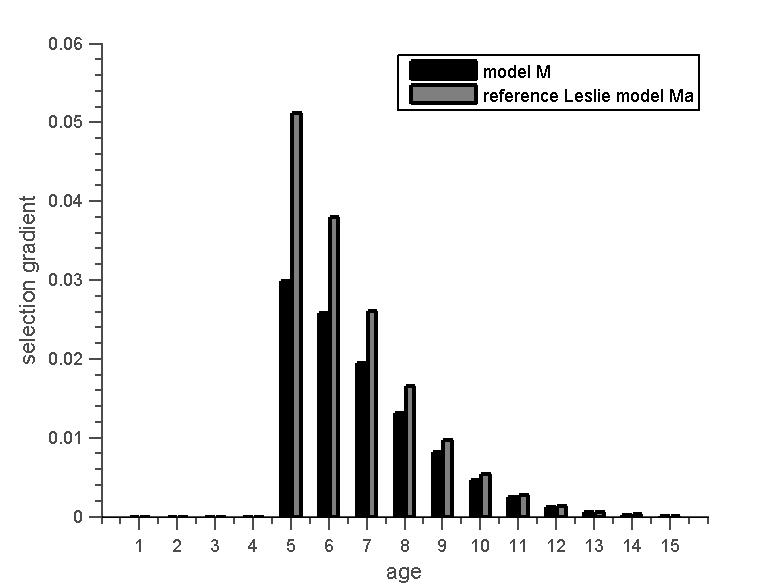
\includegraphics[scale=.25]{selgrad1.jpg}
\caption{selection gradient measured by the elasticity of ergodic growth rate to fertility rates, summed by age, for \M modeling an (\emph{age-parity}) population with physiological costs of reproduction and \Ma\ its reference Leslie matrix, which is \M folded on \emph{parity}, modeling the same population but characterized only by age. The population has maximum age $\omega=15$ and age-at-maturity $\alpha=5$. The zero-parity fertility and survival rates are 0.85. \PCoR is modeled by relatively decreasing each vital rate by $\sfrac{1}{(1+\omega -\alpha)}$ per parity.}
\label{fig:selgrad1}
\end{figure}


\subsection{\PCoR\ increases \emph{variance-effective selection gradient} for fertility of very slow organisms}
\label{sec:PCORincVarEffSelGrad_of_slow_org}
In some cases, the variance-effective selection gradient for fertility at age $a$ is actually increased by the implementation of \PCoR.  
To measure this effect, we have calculated for a range of models, varying in maximum age $\omega$ in $\lbrace2,7,12,17\rbrace$, age-at-maturity $\alpha$ in $\lbrace 1,5,9\rbrace$, in zero-parity-fertility $f(\alpha)$ in $\lbrace 0.2,0.4,0.6,0.8,1\rbrace$ and in zero-parity-survival $s(\alpha)$ in $\lbrace 0.2,0.4,0.6,0.8,1\rbrace$, the ratio, at $\alpha$ of variance-effective selection gradient between $\mathbf{M^{*}}$ the ergodic-equivalent model without any cost and the full model \M\ with the costs, and : $\frac{\sigma^{2}_{\mathcal{LRS}}}{\sigma^{*2}_{\mathcal{LRS}}}\frac{\partial \lambda}{\partial f^{*}_{a}}\frac{\partial f_{a} }{\partial \lambda }$. Among these $4 \times 3 \times 5\times 5=300$ models, 24 had a 
variance-effective selection gradient ratio below 1, and the 12 models with the lowest ratio values are presented (by increasing value of this ratio) in table \ref{tab:effvarselgrad}. As we can see, all models for which the effective selection gradient is increased by the costs of reproduction correspond to long-lived organisms (high $\omega$ and maxmimal zero-parity survival), with long reproductive periods (low $\alpha$), and among this group to those with central zero-parity fertility (which we know, since previous section \ref{ahahah}, maximizes the reduction of variance in reproductive success). \\

The mechanical explanation for such a phenomenon is simple. The buffering effect of \PCoR\ needs individual stochasticity at each time-step, i.e. a fertility rate with maximum variance ($f(\alpha) \approx 0.5$). It also needs time (high $\omega$, low $\alpha$) and life ($s(\alpha)$) to efficiently buffer this individual stochasticity. These characteristics are reflected in the difference in demographic variance, and therefore in $N_{e}$, but is not compensated by the ratio of selection gradients. This is because, for such organisms, fertility selection gradients for the model $\mathbf{M}$ with costs are definitely very low, but not much lower that the age only model $\mathbf{M^{*}}$ with no costs. Indeed, the sheer longevity of these organisms already strongly buffers fertility \citep{Morris2008}. Unrealized fertility events are not postponed, via promoted future rates like in the case of the costs of reproduction, but irrevocably lost for the individual. However, the large number of these fertility events means that failure at a particular time-step is much less costly  than it would be for a short lived or semelparous organism. Therefore, whilst further reducing the absolute selection gradients, the \PCoR\ will actually overall increase \emph{variance effective selection gradients} in long-lived organisms.\\


%%These particular cases correspond to organisms with long reproductive period (and hence with weaker effects of costs on vital rates) and with zero-parity fertility much smaller survival, in other words with a life history strategy favoring the number of reproductive events over their probability of realization (see  ). \\
 
%% This can be mechanistically understood by the fact than the selection gradient on fertility at $\alpha$ is driven by the difference in reproductive values of the various trajectories , and so is basically determined by the difference in fertility rate for the various parities of young adults (reduced by fertility itself and maximum age), whereas the variance in reproductive success incorporates fertilities at all ages with similar weights. \\


%% Table generated by Excel2LaTeX from sheet 'Sheet1'
\begin{table}[htbp]
  \centering
  \caption{Models with the 12 smallest values, in increasing order, for variance-effective selection gradient - $\frac{\sigma^{2}_{\mathcal{LRS}}}{\sigma^{*2}_{\mathcal{LRS}}}\frac{\partial \lambda}{\partial f^{*}_{a}}\frac{\partial f_{a} }{\partial \lambda }$ - among 300 models with zero-parity vital rates ranging from 0.2 to 1, $\omega$ ranging from 2 to 17 and $\alpha$ from 1 to 9}
    \begin{tabular}{rrrrrrrrrrrrr}
    \toprule
    $f(\alpha)$& 0,4   & 0,4   & 0,2   & 0,6   & 0,6   & 0,6   & 0,4   & 0,8   & 0,2   & 0,8   & 0,8   & 0,4 \\
 %%   \midrule
     $s(\alpha)$& 1     & 1     & 1     & 1     & 1     & 1     & 1     & 1     & 1     & 1     & 1     & 1 \\
    $\alpha$ & 1     & 1     & 1     & 1     & 1     & 1     & 1     & 1     & 1     & 1     & 1     & 5 \\
    $\omega$ & 17    & 12    & 17    & 12    & 7     & 17    & 7     & 7     & 12    & 12    & 17    & 17 \\
    $\frac{\sigma^{2}_{\mathcal{LRO}}}{\sigma^{*2}_{\mathcal{LRO}}}\frac{\partial \lambda}{\partial f^{*}_{a}}\frac{\partial f_{a} }{\partial \lambda }$ & 0,64  & 0,65  & 0,69  & 0,70  & 0,71  & 0,72  & 0,76  & 0,79  & 0,80  & 0,81  & 0,83  & 0,87 \\
    \bottomrule
    \end{tabular}%
  \label{tab:effvarselgrad}%
\end{table}%



%%\newpage
%%
\section{Bibliography}
\bibliography{MyEntireMendeley}


\newpage
%%\listoffigures
%%\listoftables
%%\listofboxes


\newpage

\listoftodos

\end{document}

%%%%%%%%%%%%%%%%%%%%%%%%%%%%%%%%%%%%%%%%%%%%%%%%%%%%%%%%%%%%%%%%%%%%%%%%%%%%%%%%%%%%%%%%%%%%%%%%%%%%%%%%%%%%%%%%%%%%%%%%%%%%%%%%%%%%%%%%%%%%%%%%%%%%%%%%%%%%%%%%%%%
%END of DOCUMENT
%%%%%%%%%%%%%%%%%%%%%%%%%%%%%%%%%%%%%%%%%%%%%%%%%%%%%%%%%%%%%%%%%%%%%%%%%%%%%%%%%%%%%%%%%%%%%%%%%%%%%%%%%%%%%%%%%%%%%%%%%%%%%%%%%%%%%%%%%%%%%%%%%%%%%%%%%%%%%%%%%






































\newpage

\section{oldstuddablarg}
\subsection{age structure}
In our one-sex model with a time-step of one year, we will use a simple age
 structure of $\omega=5$ age groups, with an age at first reproduction $\alpha=2$  and an age at last reproduction $\beta=4$.
 The organism we consider will have, in its reproductive years, a probability of production of one offspring which is independent of the age; we will  it the baseline fertility rate $\mathrm{f}$.
 Similarly, the organism will have a constant age-independent year-on-year survival probability $\mathrm{s}$.
This basic model can be represented by its Leslie matrix equivalent : 

%$\mathbf{L=\begin{bmatrix}0 & \mathrm{\mathrm{f}} & \mathrm{\mathrm{f}} & \mathrm{\mathrm{f}} & \mathrm{0}\\
%\mathrm{s} & 0 & 0 & 0 & 0\\
%0 & \mathrm{s} & 0 & 0 & 0\\
%0 & 0 & \mathrm{s} & 0 & 0\\
%0 & 0 & \text{0} & \mathrm{s} & 0
%\end{bmatrix}}$.

\fbox {\parbox{8cm}{
\centering \textbf{folding of MPPMs }\\ 
The folding of MPPMs is a technique to "fold" Multitrait Projection Population Matrices along one of several traits. That is to generate a matrix where transition rates only depend on a reduced set of traits but which ergodic growth rate and stage distribution is the same. When folded upon all traits but age (resp. stage) the folded matrices are called Reference Leslie (resp. Lefkovich) Matrices
}
\label{box:foldingofMPPMs}
}

\subsection{cost of reproduction modeling}
list of assumptions ?
In order to implement the cost of reproduction, we shall add  "realized fertility" as trait on top of age.  Each individual in the population will then be characterized bu a vector $\left(\mathrm{age,rf}\right)$ where  $\mathit{\mathrm{rf}}$  represent the value of the "realized fertility" trait.

We want our model to be able to implement both long-term and short-term  cost of reproduction : For a cost of reproduction where the entire reproductive  effort is taken into account, "realized fertility"  will account for parity, the total number of offspring ever-born; alternatively for a cost of reproduction where only recent reproductive effort influences future reproduction and survival, "realized fertility"  will be the success of the last reproductive event.

In practice we will create a generic "realized fertility" aggregate blending both long-term and recent successful fertility events
After each fertility event (successful or not) a reproductive adult realized  fertility will evolve as $\mathit{\mathrm{rf(\mathit{t}+1)=}\eta.\mathrm{rf(\mathit{t})}+\mathcal{F}}$ where  $\eta$ is $\mathrm{1}$ for a "realized fertility" tracking parity and $0$  for a "realized fertility" tracking the reproductive success of the latest time-step and $\mathcal{F}$  is the outcome for the reproductive adult of the reproductive event at  that time : a Bernoulli random variable of expectancy the baseline fertility  rate $\mathrm{f}$.

We also want our model to implement both cost of reproduction on (future) reproduction and cost of reproduction on survival.
We decide that this effect will be a proportional reduction of survival/reproductive rate by a factor related to the  "realized fertility" .
We will implement a In practice this means that the fertility and survival  of an individual will now be a function of $\mathrm{rs}$ ;
$\mathrm{fertility(age,rf)=}\mathsf{\mathtt{\mathrm{f.(1-\gamma.rf/\max rf)}}}$ and 
$\mathrm{survival(age,rf)=\mathrm{s.(1-\delta.rf/\max rf)}}$ 
where  $\mathrm{max rf}$ is the maximum value (on all possible trajectories) the "realized fertility" can take for the particular model and $\gamma$ and $\delta$ are impact factors comprised between 0 (realized fertility has no impact  on current fertility/survival) and 1 (when realized fertility reaches its  maximum current fertility/survival fall to 0) .
When $\eta=1$ $\mathrm{\max rf}=1$  and when  $\eta=0$ $\mathrm{\max rf}=\beta-\alpha+1$
In order to build an MPPM, it is required to know for each state, i.e. for each couple $\left(\mathrm{age,rf}\right)$ the survival and fertility rate which we just computed as well as the output states and their associated probabilities. The output state of a fertility transition will from $\left(\mathrm{age,rf}\right)$ will always be $\left(\mathrm{1,0}\right)$ as every newborn is aged 1 and has no realized fertility.
A survival transition, on the contrary, will have 2 output states :$\left(\mathrm{age+1,}\eta.\mathrm{rf}+1\right)$  with probability $\mathrm{fertility(age,rf)}$  if the fertility event is successful and $\left(\mathrm{age+1,\eta.\mathrm{rf}}\right)$ with probability $\mathrm{1-fertility(age,rf)}$ otherwise .

The resulting matrix model, in the case where $\mathrm{\eta=1,}\gamma=1$ and $\delta=0$ and $\omega=\beta=3$ and $\alpha=2$ - that is, for an age-structured population (where base fertility and  survival are independent of age) where the fertility success of the preceding time-step has nullifying impact on the current fertility - is then a 2-trait  MPPM with trait structure $\mathrm{(3,2)}$ :
$\mathbf{C}=\begin{bmatrix}0 & \mathrm{\mathrm{f}} & \mathrm{\mathrm{f}} & 0 & \mathrm{\mathrm{0}} & \mathrm{\mathrm{0}}\\
\mathrm{s} & 0 & 0  & \mathrm{s} & 0 & 0\\
0 & \mathrm{s.\mathrm{(1-\mathrm{f)}}} & 0 & 0  & \mathrm{s} & 0 \\
0 & 0 & 0 & 0 & 0  & 0 \\
0 & 0 & 0 & 0  & 0 & 0 \\
0 & \mathrm{s}.\mathrm{\mathrm{f}}  & \text{0} & 0 & \mathrm{0} & 0 
\end{bmatrix}$
\label{matC} 

Its reference leslie matrix equivalent (see section \ref{box:foldingofMPPMs}) is then :
$\mathbf{C^{fold}_{age}}=
\begin{bmatrix}
0 & f & f.(1-f) \\ 
s & 0 & 0 \\ 
0 & s & 0 \end{bmatrix} $ Thus originally age-independent rates (like fertility rates here, but it would also be the case for survival rates were $\delta$ to be switched to $1$) appear -once folded over "realized fertility" - to decrease with age once age at maturity $ \alpha $ is reached. 
 




\subsection{heterogeneity modeling}
As we just did for cost of reproduction, we can also implement individual heterogeneity in such a model via the addition of a trait. Let us call it $hetero$; the model trait structure would now be $ts=(age,rs,hetero)$.  Here, we will consider only 2 heterogeneity classes : robust and frail. And so we need to give each of those 2 classes, a fertility rate and a survival rate. We also need to define which portion of this heterogeneity is genetic, we shall call this hereditary portion $her$. The non-genetic portion $1-her$ will be distributed evenly among the heterogeneity classes. Hence, the descendant of robust (resp. frail) individual  will be robust (resp.frail) with probability $her + \dfrac{1-her}{2}$. Using those definitions, we can grow our 2-trait model $\mathbf{C}$ into a 3-trait model $\mathbf{M}$ with traits : age, realized fertility and heterogeneity class, implementing cost of reproduction in an heterogeneous population.

As described in box:foldingofMPPMs, such a model may be folded upon here heterogeneity to create  $\mathbf{M^{fold}_{age,rf}}$ a stable-state equivalent model where individuals vital rates only depend on age and realized fertility. Going one-step further we can generate $\mathbf{M^{fold}_{age}}$ the stable-state equivalent model dubbed Reference Leslie matrix where individuals vital rates only depend on age.  Such a folding allows first to easily compute the inferred fertility and survival rates by age of the studied population. Even though survival rates only depend on realized fertility and heterogeneity, and not on age in $\mathbf{M}$, the different realized fertility classes and heterogeneity class will create a gradient when population is only characterized by age. In other words, observed shapes of fertility and survival rates by age, such as in figure \ref{fig:fertsurv} , may only be due to the combined action of heterogeneity and cost of reproduction, as is the case here. 

\begin{figure}[hbtp]%[hbtp]
\centering
\begin{subfigure}{.5\textwidth}
\centering
%\includegraphics[scale=.22]{graphs/fert1Dinf.jpg}
\caption{}%
\label{fig:sub1}
\end{subfigure}%
\begin{subfigure}{.5\textwidth}
\centering
%\includegraphics[scale=.22]{graphs/surv1Dinf.jpg}
\caption{}
\label{fig:sub2}
\end{subfigure}%
\caption{fertility and survival rates of the reference Leslie matrix of 3-trait model with $\eta=\delta=\gamma=1$ with a robust class with fertility and survival of 0.95, and a frail class with fertility and survival of 0.55, with an heredity of 0.4. With regards to the each class $\omega=15, \alpha=5,\beta=13$  }
\label{fig:fertsurv}
\end{figure}%


\subsection{Variance of LFR calculation ? ici ou apres }
\subsection{stochastic growth rate ? ici ou apres }

\newpage
\section{results}
We have built, for each series of potential parameters, 3 MPPMs \M{}, \Magerf{} and \Mage{}, the second and third one resulting from the first one via folding (see box \ref{box:foldingofMPPMs}). Those 3 matrices are equivalent at the ergodic stable state, which mean they share the same ergodic growth rate \lam{} and the same ergodic stage distribution \w{}. They also share the expectation of Lifetime Reproductive Success, sometimes called \Rzero or $\mathbf{NRR}$ (see discussion, proof etc ... in section \ref{sec:noteonR0}).  We can now use those 3 matrices in order to gauge the impact of CoR (CoR in an heterogeneous environment, to be precise ) on several parameters driving evolutionary force :


\begin{itemize} [label=--]
\item \textbf{selection gradients }(see section \ref{sec:signif_evolutionnary_matrices }) measure the strength of the  force of selection on particular trait or set of traits. In matrix models and more generally, MPPMs, selection gradients are sensitivity or elasticity of ergodic growth rate \lam - taken as fitness - to a transition or vital rate or combination of transition/vital rates. \M, \Magerf{} and \Mage{} share the same ergodic growth rate \lam{} and the same ergodic stage distribution \w{} but different selection gradients, indicating the selection will act with varying strength on the 3 different modeled populations.   
\item \textbf{the variance of lifetime reproductive success } the variance of lifetime reproductive success (LFR) influences the Efficient Population Size and the differential in forces between natural selection and drift (TOUTTTT POURRRRIIII). The expectancy of LFR or \Rzero or $\mathbf{NRR}$ is the same between \Mage{} and \Magerf{}; and also with \M{} when at the stable state. This does make sense when considering \Rzero as an alternative fitness measure to \lam. If \Rzero can be considered a weaker fitness measure \lam because it only measures growth rate per generation and not in absolute time, it has the merit of being easier to make sense of when zooming in from the population level to the individual level. Each individual has its own LFR and if on average those individuals amount to \Rzero, the variance between individual's LRF also has an impact on a population's fate \citep{Giaimo2014} .In our model, the variance of LFR varies for the 3 populations modeled by those 3 matrices.    
\item  \textbf{stochastic growth rates } stochastic growth rates in a variable environment. Matrices \M , \Magerf{} and \Mage{} all share the same ergodic growth rate. However even when encompassing averaged vital rates over long period of times, those only represent the behavior of the relevant populations when in a constant environment.  In reality vital rates may change each time-step, sometimes radically. The general theory of population projection matrices in variable environments tells us that, given an ergodic set of matrices representing various environments, that each simulation will , apart on a set of size 0, tend towards a single rate : the stochastic growth rate \citep{Tuljapurkar1986,Tuljapurkar1986a,Tuljapurkar1980,Lewontin1969}. How will our 3 populations behave when the formerly considered constant "good" environment, can be (rarely but strongly) depressed ? 
\end{itemize}

 
\subsection{selection gradients when CoR  and heterogeneity is incorporated}
In evolutionary demography, selection gradients are often equated with sensitivities or elasticities of ergodic growth rate to specific parameters, which often happen to be fitness components (i.e. vital rates) themselves. Sensitivities represent additive or cumulative selection gradient and elasticities multiplicative. Classical (i.e. 1-trait) Population  Projection Matrices  contain transitions rates than can be directly identifiable with fertility rates and survival rates and as such the sensitivities/elasticities of such rates can be directly calculated from the right and left eigen vector associated with the maximum eigenvalue which is the ergodic growth rate. In MPPMs, those vital rates are lower level parameters, as transitions contains combinations of such vital rates and other parameters. The sensitivity and elasticity of \lam{} to parameter $p$ for a  population modeled by \M{} can then be calculated : $\frac{\partial \lambda}{\partial p}=\sum_{i,j} \frac{\partial \lambda}{\partial M_{i,j}} . \frac{\partial M_{i,j}}{\partial p}  $

Vital rates by age are common to all 3 constructed matrices; either in plain sight like in the Reference Leslie Matrix \Mage; or as lower level parameters in \M{} and \Magerf{} where for instance the fertility rate for a particular triplet of traits (age, realised fertility, heterogeneity) will be found in several transitions as can be seen from matrix $\mathbf{C}$ in section \ref{matC}. As those transitions are mainly products of vital rates and other vital rates or paramters (e.g. heredity), it makes sense to use elasticities as measures of selection gradient.  It actually makes all the more sense since we want to compare elasticities of fitness components common to  \M, \Magerf{} and \Mage{} : fertilities and survivals by age are indeed easily found in \Mage; in \M{} and \Magerf{}  they are not only scattered in different positions, but also split in different components : fertility rates at a given age will vary depending on the realized fertility and the heterogeneity class. However if all, say, 5-year fertility rates increase by  .... A REFLECHIR, ET BIEN ECRIRE ... PKOI PAS LES SENSI (ca doit bien marcher aussi) POURQUOI COMMENT ON SOMME SUR TOUS LES ELEMENTS DE LA MATRICE.

As we can see from the figure \ref{fig:elasfert} below, these differences in strucures and fistribution of the fertility rates inside the matrices, leads to variations in selection gradients also. More generally, population encountering Cost of Reproduction have lower elasticities at almost every level (AND THEN SENSITIVITIES NON ... AS FERTILITY BY RATE SHOULD BE THE SAME ... AVERAGED OVER STABLE STATE SUBSTAGES...)  

\begin{figure}[hbtp]%[hbtp]
\centering
%\includegraphics[scale=.25]{graphs/fertelast.jpg}
\caption{elasticity of fertility rates by age for the 3 matrices derived from 3-trait model with $\eta=\delta=\gamma=1$ with a robust class with fertility and survival of 0.95, and a frail class with fertility and survival of 0.55, with an heredity of 0.4. With regards to the each class $\omega=15, \alpha=5,\beta=13$  }
\label{fig:elasfert}
\end{figure}

In all cases envisaged in this article, we find such an increase in selection gradient for fertilities between the heterogeneous populatin with cost of reproduction and its counterpart only categorised by age where heterogeneity and cost of reproduction have mechanilly vanished. 
Other sets of parameters than the used (above) for \ref{fig:elasfert}  however another feature appears, whereby the fertility elasticity for the intermediate model \Magerf is even higher than the fertility elasticity for \Mage. See for instance, figure fdsfsd below :

figure : 2 figures : gradient et inferred fert

This can easily be interpreted as the deceptive (trompeur) effect unravelled by \citep{VanNoordwijk1986}  (bonne quote ?) 
Indeed, in such a model, a marked heterogeneity (baseline fertilities and/or survival being very different between robust and frail individuals), i.e. a large variance in "ressource acquisition" masks and even alters the perception of the direction of the "ressource allocation" trade-off, i.e. of the cost of reproduction when this heterogeneity is no more taken as a trait, i.e. in \Magerf. It then seems that, to the contrary, for some age classes at least, succesful reproduction leads to even higher fertility rates.
Again, in all cases, the Cost of Reproduction, even in an heterogenous environment, reduces the selection gradient on fertility (see discussion)

\begin{figure}[hbtp]%[hbtp]
\centering
\begin{subfigure}{.5\textwidth}
\centering
%\includegraphics[scale=.22]{graphs/fertelast2.jpg}
\caption{}
\label{fig:elastfert2}
\end{subfigure}%
\begin{subfigure}{.5\textwidth}
\centering
%\includegraphics[scale=.22]{graphs/inferred_fert.jpg}
\caption{}
\label{fig:inferredfert}
\end{subfigure}
\caption{elasticity of fertility rates by age for the 3 matrices derived from 3-trait model with $\eta=\delta=\gamma=1$ \ref{fig:elastfert2} and inferred fertility in \Magerf  \ref{fig:inferredfert} with a robust class with fertility and survival of 0.90, and a frail class with fertility of 0.15 and survival of 0.85, with a heredity of 0. With regards to the each class $\omega=15, \alpha=5,\beta=13$}
\label{fig:ressourceallocation}
\end{figure}



\subsection{variance of Reproductive success in CoR and heterogeneous environment }

The previous section considers the effect of vital rates and potential implemented trade-offs and additional traits at the level of the population. However, the transition rates and fertility rates in such models only reveal the expectations of what are really biological stochastic processes : in our models where individuals can only produce one offspring at most per time-step, both survival-per-timestep and reproduction-per-timestep are Bernoulli processes of parameter the implemented rates. Let us note here, that if this make every transition rate in \Mage the expection of a corresponding Bernoulli process, it is not the case of the higher complexity models, like \M : For each particular state, the set of all fertility (resp. survival) transitions towards every offspring (resp. repro success classes) classes, from that state, should be from an individual stochasticity point of view , altogether considered as one Categorical/Multinoulli  (or genereralized bernoulli) process which distribution is described by the various transition rates.

There are various way to measure individual stochasticity. In a Leslie matrix model, individuals can take various trajectories : it can die at any time before the maximum lifespan implemented and reproduce or not every time step. If all fertilities and survivals are strictly comprised between 0 and 1, and if the maximum of number of offspring per lifetime is 1, then they are $2^{n+1} -2$ differentiable individual trajectories allowed by the model. This quickly becomes a very large number, that will only increase when other traits are added. 

Particular properties of these trajectories have much smaller outputs and particular significance from a demographic and evolultionary standpoint, in particular the age at death and the lifetime reproductive success.  The moments of age at death , which can all be directly reached from the fundmanetal matrix of the model, provide information on the survival heterogenity of the population. The moments of the LFS integrate that information (dead invidual rarely reproduce) and tell us many thing about the fitness of the population. The expectation of the LRS, which is equal to \Rzero  (for models with only one type of offspring and in general providing the correct computation of \Rzero is used ;see section \ref{sec:noteonR0}) obtained from the model matrix itself, split into fertility and survival transitions, and its associated next-generation matrix R, has indeed long been debated and used as an alternative measure of fitness to the ergodic growth rate (discusions dfdfdsfdsfds ).  It has the drawback of losing track of chronological time - a real shortcoming when dealing with models with strongly overlapping generations; but has for itself the advantage of being both a population measure (\Rzero is the average number of offsprings a random individual is expected to have during its lifetime) and an indivual one. It is easy to understand the meaning of the LRS of an individual, much less its individual growth rate, despite the efforts of some (lhjhjhkjhj). The variance in indivual fitness, with vast implications both demographic and evoltuionnary (see in intro ??), will have to measured by the variance in LFS.\\
Contrary to the first moment, 2nd and further moment of LFS can be directly drwn from the model matrix and its affiliates. In order to compute it, we will make use of markoc chain with reward as pionnered by (ref ref) and first applied to ecology by (ref ref). Shortly, this technique two instruments: 
\begin{itemize} \item  the extended matrix of transitions which is the matrix of transitions augmented by additional state "death". This matrix fully describes the various survival trajectories  any individual in the population can take.
				\item and the familty of reward matrix $\mathbf{Rw^{k}}  $ where $\mathbf{Rw^{k}_{ij}}  $ is the $k^th$ moment of the distribution of the particular reward - in our case an offspring - an individual can grab when transitioning for state {j} to state {i} and accumulate with rewards already awarded to him.  In an MPPM  like \M or \Magerf the survival transitions may (and \textit{do} in our case) depend on the actual realization of fertility event. This implies that, in a model implementing CoR, the reward for transitioning from j to i, will not depend only on j, as it did in earlier application of markov rewards to biology and where thus the reward matrices is the replication of a single line (ref ref). In a CoR model, for each start state {j=(age,rf,het)} only 3 outputstates are possible : 
	\begin{itemize} \item $i1=(age+1,rf+1,het)$ for survival and succesfull fertily event,
				    \item $(i2=(age+1,rf,het)$ for survival and failed  fertily event and
				    \item $(d=(death)$ if the individual dies. 	\end{itemize}
 The associated entries of the Rw matrices will then be
 \begin{itemize} \item $\mathbf{Rw^{1}_{i_{1}j}}=1$ as this is a fixed reward (always a reproductive event),
 				 \item $\mathbf{Rw^{1}_{i_{2}j}}=0$, this is also a fixed reward (never a reproductive event) and
 				 \item $\mathbf{Rw^{1}_{dj}}=fert(j)$, the 1st moment of the relevant bernouilli process of paramter $fert(j)$.
 \end{itemize}    
 
In all three cases, the 2nd and further moments are equal to the first one. This means $\mathbf{Rw^{1}}=\mathbf{Rw^{2}}=\mathbf{Rw^{3}}=...$  \end{itemize}
				
We then run backwards in time (age) and accumulate the rewards from late till young (A CHECKER ET A PRECISER ...) until it converges towards the family of vectors $\mathbf{accrw^{k}}  $  where $\mathbf{accrw^{k}_{i}}$ is  the $k^{th}$ moment of the lifetime accumulated reward starting from state {i}. (MIEUX COMPRENDRE LE RPINCIPE BACKWARD, RELIRE PAPIER CASWELL, ET PREPARER UNE XPLICATION (PEUT ETRE POUR SUPMAT))

If $\mathbf{r^{k}}  $  is the vector of entries of $\mathbf{accrw^{k}}  $ corresponding to the kth moment of LFS for offsprings,  the vector of expectancy of LRS for each offspring class is $  \mathbf{e_{LFS}}=\mathbf{accrw^{1}}$  and the vector of variance of LRS for each offspring class is $  \mathbf{var_{LFS}}=\mathbf{r^{2}}-\mathbf{r^{1}}\circ\mathbf{r^{1}}$ where $\circ $ is the hadamard, termwis, product.
As can be expected, the $\mathbf{e_{LFS}}$ is the sum of expected number of offspring of each heterogenity class (let's call $off1$ and $off2$ the two offspring states in \M),i.e. $\mathbf{e_{LFS}} = \begin{pmatrix}
\mathbf{R_{off1,off1}}+\mathbf{R_{off2,off1}}\\ 
\mathbf{R_{off1,off2}}+\mathbf{R_{off2,off2}}
\end{pmatrix}  $
ON DIT DEJA CA DANS LA NOTE CORRESPONDANTE NON ?
\\We can then, as we did for \Rzero already in section \ref{sec:noteonR0}, calculate the expected LRS for an individual taken at random (in the stable-state population where the relative abundances of offspring classes are $w_{off1}$ and $w_{off2}$) :
$\mathrm{e_{LFS}} = w_{off1}.\mathbf{e_{LFS}}_{off1}+w_{off2}.\mathbf{e_{LFS}}_{off2}  $
\\ In a similar fashion, we can weight elements of $  \mathbf{var_{LFS}}$ by the abundance weights $w_{off1}$ and $w_{off2}$ but the formula is only slighlty more complicated. If $\mathcal{LRS}$ is the random variable representing the LRS of a random individual in the offspring population,$\mathcal{LRS_\mathrm{1}}$ is the random variable representing the LRS of a random individual in offspring class 1 and $\mathcal{LRS_\mathrm{2}}$ is the random variable representing the LRS of a random individual in the offspring class 2 then we know that  :
$  \mathrm{var_{LFS}} = Var(\mathcal{LRS})=E(\mathcal{LRS}^2)-E(\mathcal{LRS})^2$ where $E(\mathcal{LRS})=\mathrm{e_{LFS}}$ that we just calculated and $ E(\mathcal{LRS}^2) $ is the square of the exoectation of LRS of all offspring at stable state, and such $ E(\mathcal{LRS}^2)= w_{off1}.E(\mathcal{LRS_\mathrm{1}}^2) +w_{off2}.E(\mathcal{LRS_\mathrm{2}}^2)$ which can be rewritten $ E(\mathcal{LRS}^2)= w_{off1}.(Var(\mathcal{LRS_\mathrm{1}}) + E(\mathcal{LRS_\mathrm{1}})^2) +w_{off2}.(Var(\mathcal{LRS_\mathrm{2}}) + E(\mathcal{LRS_\mathrm{2}})^2)$ and thus 
\[ \mathrm{var_{LFS}} =w_{off1}.\mathrm{var_{LFS_1}}  +w_{off2}.\mathrm{var_{LFS_2}}+w_{off1}.\mathrm{e_{LFS_1}}^2+w_{off2}.\mathrm{e_{LFS_2}}^2-\mathrm{e_{LFS}}^2\]
which we can interestingly decompose :
\[ \mathrm{var_{LFS}} = \mathrm{var^{sto}_{LFS}}  + \mathrm{var^{het}_{LFS}}\]
where $ \mathrm{var^{sto}_{LFS}}  =w_{off1}.\mathrm{var_{LFS_1}}  +w_{off2}.\mathrm{var_{LFS_2}}$ is the portion of the overall variance due to indivual stochasticity 
and $  \mathrm{var^{het}_{LFS}} =w_{off1}.\mathrm{e_{LFS_1}}^2+w_{off2}.\mathrm{e_{LFS_2}}^2-\mathrm{e_{LFS}}^2$ is the portion due to the heterogeneneity (implemented) in the population.




				
%variance_LRO=varrho_off'*wMoff  +  exprho_off'.*exprho_off'*wMoff  - (exprho_off'*wMoff)^2 ;%;
%variance_LRO_stocha=varrho_off'*wMoff  ;%;
%variance_LRO_het = exprho_off'.*exprho_off'*wMoff  - (exprho_off'*wMoff)^2 ;%;
				
				
				






\subsection{Cost of Reproduction in variable environment}

So far, we have compared,in a constant environment, populations incorporating (short or long term) cost of reproduction (on reproduction or survival), modeled by $\mathbf{M}  $  ... 
... with their "equivalent" populations characterized only by age  (and hence with neither cost of reproduction nor individual heterogeneity ) modeled by $ \mathbf{M_{age}}  $.  

 We have showed that even though both populations the same asymptotic behavior (same growth rate, same stable population structure, same expectancy of lifetime reproductive success), the population models implementing cost of reproduction show reduced fertility selection gradient compared to their reference Leslie model, and reduced variance in reproductive success.
 
We shall now consider variable environments, and compute the behavior of those populations - that are "equivalent" in a constant environment at the stable state - when subject to rare but very stressful adverse environment bouts.

In our particular model, we will consider the matrices built and computed in the previous paragraphs as representative of a general/good environment that is preponderant for the species studied. However sometimes, but rarely say $ \theta $ of the time, the environment can turn so bad the species do not reproduce and survives very poorly (all individuals have a very low survival rate, we call $ s_{b} $ equal to the lowest survival rate possible of all heterogeneity and all realized fertility at the good environment), we model this environment with matrix  $\mathbf{0_{age,rf,het}}$. We consider that both environments are i.i.d.

We can also provide $ \mathbf{M_{age,rf}}  $  and $ \mathbf{M_{age}}  $  with such "poor environment" counterpart $ \mathbf{0_{age,rf}}$ and $ \mathbf{0_{age}}$ where all fertilities are zero and survival is $ s_{b} $ . We can then compare the different trajectories of the different simulations as we in figure \ref{fig1}.Let us note here  that as various matrices 
$\mathbf{M}$ , $\mathbf{M_{age,rf}}$ and $\mathbf{M_{age}}$ are all folded versions of one another according to $\mathbf{M}$
, such is the case also for $\mathbf{0_{age,rf}}$ and $ \mathbf{0_{age}}$ which are folded versions of $\mathbf{0_{age,rf,het}}$ along $\mathbf{M}$. This means that the matrices used to generate \ref{fig:sub2} are folded versions of the matrices used to generate  \ref{fig:sub1} according to  \ref{fig:sub2} . This means that in environment that is constantly "good" they share the same ergodic behavior, as well as-obviously- when the environment is constantly bad. However when the environment is allowed to shift from one environment to the other, those asymptotic behaviors differ. 

  As the good environment is predominant we have decided to fold the 3-trait matrices(s) alors $\mathbf{M}$. Considering that the average transition rates over time in my population are now those of $ \mathbf{\bar{M}}=(1-\theta)*\mathbf{M}+\theta*\mathbf{0_{age,rf,het}} $, we can also use a different version of $\mathbf{M_{age}}$ computed from $\mathbf{M}$ via folding over $ \mathbf{\bar{M}} $. ($\mathbf{0_{age,rf}}$ and $\mathbf{0_{age}}$ would remain the same as $\mathbf{0_{age,rf,het}}$'s do not depend on heterogeneity or realized fertility.

\begin{figure}[hbtp]%[hbtp]
\centering
\begin{subfigure}{.5\textwidth}
\centering
%\includegraphics[scale=.22]{graphs/simulM_nohet.jpg}
\caption{}
\label{fig:sub3}
\end{subfigure}%
\begin{subfigure}{.5\textwidth}
\centering
%\includegraphics[scale=.22]{graphs/simulMage_nohet.jpg}
\caption{}
\label{fig:sub4}
\end{subfigure}
\caption{20 simulations for a population where $\theta=3pct $ of the time the environment is depressed to 0 fertility and very low (equal) survival either integrated in M (Magerfhet)   }
\label{fig1}
\end{figure}

 As we can see  in \ref{fig1} both systems ($\mathbf{M}$ and $\mathbf{0_{age,rf,het}}$ for \ref{fig:sub1} and $\mathbf{M_{age}}$ and $\mathbf{0_{age}}$ for \ref{fig:sub2}) encounter the same extinction events : indeed those are due to the possible successions of "poor" environments. Successions are possibles as the environment is i.i.d : at any time, the environment does not depend on environment's history, not even on the environment at the last time-step, but only on the "roll of a dice". If the dice rolls on "poor" for more times in a row than $ \beta $ (the age at last reproduction), then the population goes extinct. As the environment is the same for both systems (same simulation number implies same environments) the same simulations will go extinct or survive.  However the rates at which the 2 populations would recover from such catastrophic events and , in fine, grow over time - that is, the stochastic growth rate implied - are somewhat different : event though positive and negative sequences of environments are the same for both systems (for the same reason simulations that go extinct are the same) we can see that for each simulation the growth rate is higher for \ref{fig:sub1} than for \ref{fig:sub2}. In 4 cases in \ref{fig1} we have simulations yielding, from an initial population of 1, and after 8000 time steps, total populations inferior to one (the magic of demography!) when using the  $ (\mathbf{M_{age}}, \mathbf{0_{age}}  ,\theta )$ system, whilst that population is the 000S for $ (\mathbf{M}, \mathbf{0_{age,rf,het}}  ,\theta )$ system 
  In other words, the stochastic growth rate of the $ (\mathbf{M}, \mathbf{0_{age,rf,het}}  ,\theta )$ system is superior to those of the $ (\mathbf{M_{age}}, \mathbf{0_{age}}  ,\theta )$ system whereas $ \mathbf{M}$ and $ \mathbf{M_{age}}$ have the same ergodic growth rate  (as well as $ \mathbf{0_{age,rf,het}} $ and $\mathbf{0_{age}}$). Cost of Reproduction increases stochastic growth rate in variable environments for a model compared to its reference leslie model. If,in a constant environment where survival and fertility rates are fixed, and hence the transitions rates towards the different "repro success" classes,   such a model may be "equivalent" to a Leslie matrix where cost of reproduction outcrops in the negative slope of survival and/or fertility with age;  this relationship doest not hold when faced with environmental variability. Cost of Reproduction  acts as a buffer :when suddenly faced with a catastrophic environment preventing reproduction,  all individuals at the beginning of their reproductive period will remain in the "low reproductive success" class, allowing them to reproduce more when the environment is back to normal that the Leslie equivalent population.


\newpage
\section{discussion}
\subsection{selection gradients and senescence theory}
As seen in the first part of the results (ref) in all cases, the Cost of Reproduction, even in an heterogenous environment, reduces the selection gradient on fertility. 
This implies that, this trade-off, which is an obvious part of the disposable soma theory's physiological compromises, actually accelrates the senescence of the individuals and on average of the population and the species (this is directly implemented in our model \M where fertility and/or survival rate decrease with (recent or lifetime reproductive success), but, doing so, decreases the slope of the selection gradient by age and therefore reduces the anticipated apparition of antogonistically peiotropic mutations and the accumulation of deleterious mutations until after the reproductive period. 
the selection gradient on selection by age will also be reduced during the (especially the beggining of the) reproductive period, but will decrease all the more strongly (in our simple model where no intergerational transfer apart from the cost of reproduction itself, is modeled) in the post-reproductive period if any.

\subsection{individual stochasticity, reduction in LRS variance and genetic drift}%


\subsection{resilience in variable environments}


\newpage
\newpage
\section{Note on the signification of the evolutionary meaning of a matrix projection model}
\label{sec:signif_evolutionnary_matrices }
Matrix population models allow to compute sensitivities and elasticities of the ergodic growth rate $\lambda$ to matrix entries (first level sensitivity analysis) and - via those - to  any parameter influencing those matrix entries (2nd level sensitivity analysis). 

In one trait population projection matrices (age-structured (Leslie) or stage-structured (Lefkovitch) for instance), and considering $\lambda$ as a fitness measure, those 2nd level sensitivities have early been identified with selection gradients (van tienderen, shyu caswell 2014 quoting Caswell 2001 ? autres ? ... ). 

Indeed those sensitivity rates measure the local slope of fitness as a function of a fitness component (fertility or survival rate) (taken here as a trait), and as such indicate which of those fitness components are  most beneficial to select to maximize $\lambda$. 

Those selection gradients then need to be compounded by their additive genetic variance/covariance in order to estimate the longer term effect of natural selection as we know from the one-dimensional and multidimensional versions of the Breeders/Price equation (Price, Lande ...).

The development of multitrait population projection matrices, where individuals are characterized by several traits (that can be of varying nature) ,  by Caswell and Coste , allows to incorporate a hereditary, hence genetic,  component in the matrix. 

 In a Leslie matrix for instance, one can had a "size at birth trait" to the already-existing age trait; where the new trait influences at least one of the survival/fertility rates.  
 
 The correlation between the major fitness components and the new trait is akin to the selection differential <y,w> of the breeders equation.  The distribution of offspring may be the same for all - a generic distribution
- or depend on the "size at birth" trait (directly or indirectly if it depends on age which distribution is  a function of "size at birth"); in this case, there is a genetic/hereditary component implemented in the model. 

 The sensitivities issued from such a model may not be called "selection gradients"  as they already incorporate the genetic basis of the studied trait variance (the non-genetic basis being the a generic distribution); we shall call  them "natural selection gradients". 
 
Let's note here that it may seem surprising that a selection/evolution process  as the one implemented in the such a matrix with hereditary trait would  lead to an ergodic stable state (as most MPPM do , see Coste et al).
 This is because, in a such a model : selection (the influence of the trait on fitness component and hence on the lifetime reproductive output ...) and  evolution thanks to the genetic transmission of this selection to the next generation () occur in an environment where phenotypic variance is forced at a minimum level (the generic distribution) counteracting in a way the  natural selection process.


\newpage
\section{Note on trade-offs in matrix population models}
Trade-offs have long been studied through (or related to) population projection matrices models.

 The first approach was to consider that at the stable state such a modeled population has reached an ESS where $\lambda$ is (locally) maximized.
 
 If all entries of a Leslie matrix, for instance, that is, the survival  probabilities and fertility rate at each age, influence positively the Malthusian fitness, it is because those rates are themselves function of  lower-level parameters that have varied effect on the fitness components.
And hence the relationship between those fitness components, via the lower level  parameter, established trade-offs (quote qui ?).\\
 A slightly different approach, but similar in concept, is to consider that  each pair of sensitivities of matrix entry is itself a trade-off : If my  population is at an ESS, and if elasticity of survival rate at 2 yrs is  twice the elasticity of the fertility rate at 12yrs, it means that there  is a trade-off of slope 2 between those components; an increase of 2pcent of  the first rate would imply a decrease of 1pcent of the second rate, and hence keep $\lambda$ constant.(quote caswell).
 
Those approaches analyses trade-offs that are expected to be there (under  the assumption of ESS) or to detect the force of a potential trade-off  from the sensitivities of the fitness components with no consideration  for the sensitivity of the trade-off itself.
 
However, it is actually possible to implement a trade-off in a matrix model,  using the multitrait capabilities of MPPMs to add a specific trait and/or  a specific trade-off measure (the parity for the trade-off studies here  known as the cost of reproduction).
This allows to model most type of trade-offs as detailed in the seminal but vastly ignored topology of trade-offs by Stearns (stearns, 19...) ; chiefly
- indivual trajectory trade-off that determine the directions taken by an
 individual at each time-step as a function of its recent or entire history. 
 Most trade-offs related to a budget (Lee ...) are of this category.
 An individual that has used a lot of energy to grow will have less energy
 to reproduce over the next time steps (modulo its robustness) .....
 Those trade-offs are mechanistic and do not need any genetic basis to occur  and remain in a population.
- trade-off with a genetic (pleiotropy, linkage ...) basis which occur mainly at the species/population level.
A trade-off may actually be part of both categories and its genetic basis  will be implemented via the hereditary portions of the trade-off's characteristics.


\newpage
\section{note on \texorpdfstring{$\boldsymbol{\mathcal{R}_{0}}$}{Lg}  in matrix models with several classes of offspring}
\label{sec:noteonR0}

The definition, meaning and calculation of the extension of $\mathcal{R}_{0}$  - originally an epidemiological concept - to structured population models,  in the case where offspring are not characterized by a single state -  i.e. when the matrix of fertility rates $\mathbf{F=M-T}$  contains several non-zeros lines - are still unclear despite numerous works on the subject \citep{Heesterbeek2002,DeCaminoBeck2008,Caswell2011b,Cushing1994} 
In the case where a population dynamics is only described by the population's  Net Generation Matrix $\mathbf{\boldsymbol{R=\mathrm{\left\{ \mathrm{R_{\mathit{i,j}}}\right\} }}}$ - that provides for a random offspring of category $\mathit{j}$  the number $\mathrm{R_{\mathit{i,j}}}$ of offspring of category $\mathit{i}$ it is expected to have during its entire life - we do agree that the Net Reproductive Rate $\mathrm{NRR}=\max\mathit{eig\mathrm{(\mathbf{R\mathrm{)}}}},$ the population growth rate per generation (whatever the interpretation of  such a measure when generations massively overlap), measures mean lifetime  reproductive success : 

$\mathrm{E(\mathfrak{\mathcal{LRS}})}=\max\mathit{eig\mathrm{(\mathbf{R\mathrm{)}}}}  $
Indeed, such a population will tend toward a stable-state with regard to
 generation time, of growth rate the maximum eigenvalue $\mathrm{NRR}$
 and relative abundance vector of offspring categories $\mathbf{w^{R}}$
the associated right-eigenvector 
\begin{equation}
\mathbf{R.}\mathbf{w^{R}}=\mathrm{NRR.}\mathbf{w}\mathbf{^{R}}
\label{eq:R0eq1}, 
\end{equation}
, with $\sum\mathrm{w_{\mathit{i}}^{R}}=1$.  Then, by summing all elements on each side of (1), one can show that $\sum_{i,j}w_{j}^{R}.\mathrm{R}_{i,j}=\mathrm{NRR}.$  The Net Reproductive Rate is the $\mathrm{\mathbf{w^{R}}}$-weighted sum of all $\mathbf{R}$ transitions i.e.
 the $\mathrm{NRR}$  is the expected number of offspring from a random offspring, providing  the distribution of offspring within categories follows the generation  abundance vector.
This is different from the expected number of offspring of a random individual  at a given time $\mathit{t}$ , but a best guess when only $\mathbf{R}$  is known and a relatively good approximation of $\mathrm{E(\mathfrak{\mathcal{LRS}})}$ when the distribution of reproductive output of the studied organism is very small with regards the organism life-history schedule.

When the time-step transition matrix $\mathbf{M}$ is known, then the expectancy of life-reproductive output can be computed  by combining elements of both the generation growth equation \eqref{eq:R0eq1} and the  time-step growth equation : 
\begin{equation}
\mathbf{M.}\mathbf{w^{M}}=\mathrm{\lambda.}\mathbf{w}\mathbf{^{M}}
\end{equation}
 ,where $\mathrm{\lambda}=\max\mathit{eig\mathrm{(\mathbf{\mathrm{\mathbf{M})}}}}$  and 
$\sum\mathrm{w_{\mathit{i}}^{M}}=1$ . At the stable state, in a population characterized by $\mathrm{n}$  states where the first $\mathrm{off}$
 states represent offspring, the relative abundances of offspring is given
 by 
\newpage
\section{note on elasticities and sensitivities of fertility rates in CoR in heterogenous populations}
ON PEUT AUSSI TOUT SIMPLEMENT DIRE QU'EN SOMMANT DES ELASTICITES DE PARAMETRES (INDEPENDENTS LES UNS DES AUTRES) ON REGARE L IMPACT D UN MOUVEMENT PARALLELE DE TOUS LES CONSTITUENTS...


We wish to compare the selection gradients of fertility for the 3 populations modeled by the 3 matrices:  \M, \Magerf{} and \Mage.
To be more precise, we wish to compare the selection gradients of fertility for each age class, i.e. $fert(age)$ as $age$ is the only input shared by fertility rates to be found inside \M, \Magerf{} and \Mage. 

\begin{sloppypar}
In \Mage{}, the first line of the Leslie matrix, provides us with $fert_{\mathbf{M_{age}}}(age)$ and hence the first line of sensitivity matrix $\mathbf{S_{age}} =\mathbf{v}.\mathbf{w}'$  (resp. elasticity matrix $\mathbf{E_{age}} =\frac{1}{\lambda}  \mathbf{S_{age}} \otimes \mathbf{M_{age}}$) with $sfert_{\mathbf{M_{age}}} (age)=\frac{\partial \lambda}{\partial fert_{\mathbf{M_{age}}}} $ the sensitivity of \lam{} to $fert_{\mathbf{M_{age}}}(age)$ (resp. with $efert_{\mathbf{M_{age}}} (age)=\frac{fert_{\mathbf{M_{age}}}}{\lambda}.\frac{\partial \lambda}{\partial fert_{\mathbf{M_{age}}}} $the elasticity of \lam{} to $fert_{\mathbf{M_{age}}}(age)$). We additionally know that \lam{} being an homogeneous function of all matrix entries, that the sum of all elements of an elasticty matrix sum to 1. In the particular case of \Mage{} where those entries are $fert_{\mathbf{M_{age}}}(age)_{_{age=1 ... \omega}}$ and $surv_{\mathbf{M_{age}}}(age)_{_{age=1 ... \omega}}$ we can write $\sum_{age=1}^{\omega} esurv_{\mathbf{M_{age}}} (age)+\sum_{age=1}^{\omega}efert_{\mathbf{M_{age}}} (age)  =1 $; allowing to consider each of these components as the contribution of the relevant vital rate by age to fitness (see sdfsdfds for discussion on dfsdfsd) 
\end{sloppypar}%

Two issues occur when considering \M{} and \Magerf{} :
\begin{itemize} [label=--]
\item \begin{sloppypar}
the fertility rate (and survival rate) of each specific state  $fert_{\mathbf{M}}(age,rf,het)$ (resp. $fert_{\mathbf{M_{age,rf}}}(age,rf)$) appear in several positions in \M{} (resp. in \Magerf{}).
 This implies that, unless in particular cases,$\sum_{age,rf,het} esurv_{\mathbf{M}}(age,rf,het) + efert_{\mathbf{M}}(age,fr,het)\neq 1 $ . Those elasticities cannot then be considered as individual independent contribution to \lam. However as there is at most one fertility rate and at most one survival rate in each entry of \M (or \Magerf), the $esurv_{\mathbf{M}}(age,rf,het)$ can be scaled to 1 and considered as contributions to .... (PAS TROP SUR LA ...A RECHECKER PLUS TARD)   .Let us note here that $fert_{\mathbf{M}}(age,rf,het)$ and $surv_{\mathbf{M}}(age,rf,het)$ only appear however in transitions from that state $(age,rf,het)$ to onward states, i.e. in \M{} in the column corresponding to state $(age,rf,het)$.\end{sloppypar}%
\item
\begin{sloppypar}
 the fertility rate we find in \M{} and \Magerf{} are not actually   $fert_{\mathbf{M}}(age)$ or $fert_{\mathbf{M_{age,rf}}}(age)$; these rates do not appear in the matrices. They are abundances weighted averages of the $fert_{\mathbf{M}}(age,rf,het)$ : $fert_{\mathbf{M}}(age)=\frac{\sum_{rf,het} w_{age,rf,het}.fert_{\mathbf{M}}(age,rf,het)}{\sum_{rf,het} w_{age,rf,het}} $. We then need to decide the meaning we want to give to $\frac{\partial \lambda}{\partial fert_{\mathbf{M}}}$ (an improper mathematical notation, as, again, $ fert_{\mathbf{M}} $ cannot be found in \M). There is an infinity of ways the components of  
$fert_{\mathbf{M}}(age)$ can evolve to influence its output. However two basic co-variations that make sense biologically stand out \end{sloppypar}:
	\begin{itemize} [label=--]
	\item an equal increase/decrease in all fertiliry rates constituting $fert_{\mathbf{M}}(age)$
	\item a proportionnal increase/decrease in all fertiliry rates constituting $fert_{\mathbf{M}}(age)$
	\end{itemize}
In the first case, this means the difference every pair of fertility rate is constant through time. That is, one can write $fert_{\mathbf{M}}(age,rf,het)=K(age,rf,het)+f(age)$, i.e. each for each age class, every fertility rate is the sum of a function of age $f$ which can vary, and a constant (through time) function of $(age,rf,ht)$. Then $fert_{\mathbf{M}}(age)=\frac{\sum_{rf,het} w_{age,rf,het}.fert_{\mathbf{M}}(age,rf,het)}{\sum_{rf,het} w_{age,rf,het}}=\frac{\sum_{rf,het} w_{age,rf,het}.K(age,rf,het)}{\sum_{rf,het} w_{age,rf,het}}+f(age)$. As an abundance $w_{age,rf,het} $ is a function of fertilities and survival for states where age is below $age$ (see dffdfdf), the entire first part of this equation does not vary through time :  $fert_{\mathbf{M}}(age)=K'(age,rf,het) +f(age)$. Then $fert_{\mathbf{M}}(age,rf,het)=K(age,rf,het)+fert_{\mathbf{M}}(age)-K'(age,rf,het)$ giving $\frac{\partial fert_{\mathbf{M}}(age,rf,het)}{\partial fert_{\mathbf{M}}(age)}=1 $ 
\\In that case, and only in that case, where  $\frac{\partial \lambda}{\partial fert_{\mathbf{M}}}$ is understood as the influence of a parallel move for each age, of all multitrait fertility rates constituting $fert(age)$, do we then have, via the chain rule : $\frac{\partial \lambda}{\partial fert_{\mathbf{M}}(age)}=\sum_{rf,het}\frac{\partial \lambda}{\partial fert_{\mathbf{M}}(age,rf,het)}*\frac{\partial fert_{\mathbf{M}}(age,rf,het)}{\partial fert_{\mathbf{M}}(age)}=\sum_{rf,het}\frac{\partial \lambda}{\partial fert_{\mathbf{M}}(age,rf,het)}$.: The sensitivity of fertility by age in \M  (understood as a parallel move off all constituent fertility rates) is the sum of all elasticities for states constituting that age class. 



This does hold in the second case, where the ratio between every pair of fertility rate is constant through time : $fert_{\mathbf{M}}(age,rf,het)=K(age,rf,het)*f(age)$. Then $fert_{\mathbf{M}}(age)=\frac{\sum_{rf,het} w_{age,rf,het}.fert_{\mathbf{M}}(age,rf,het)}{\sum_{rf,het} w_{age,rf,het}}=\frac{\sum_{rf,het} w_{age,rf,het}.K(age,rf,het)}{\sum_{rf,het} w_{age,rf,het}}*f(age)=K'(age)*f(age)$. Then $fert_{\mathbf{M}}(age,rf,het)=\frac{K(age,rf,het)}{K'(age)}*fert_{\mathbf{M}}(age)$ giving $\frac{\partial fert_{\mathbf{M}}(age,rf,het)}{\partial fert_{\mathbf{M}}(age)}=\frac{K(age,rf,het)}{K'(age)}*fert_{\mathbf{M}}(age) $ 

In that case, and only in that case, where  $\frac{fert_{\mathbf{M}}}{\lambda} \frac{\partial \lambda}{\partial fert_{\mathbf{M}}}$ is understood as the influence of a proportional move for each age, of all multitrait fertility rates constituting $fert(age)$, do we then have, via the chain rule : $\frac{fert_{\mathbf{M}}(age)}{\lambda} \frac{\partial \lambda}{\partial fert_{\mathbf{M}}(age)}=\frac{fert_{\mathbf{M}}(age)}{\lambda}\sum_{rf,het}\frac{\partial \lambda}{\partial fert_{\mathbf{M}}(age,rf,het)}*\frac{\partial fert_{\mathbf{M}}(age,rf,het)}{\partial fert_{\mathbf{M}}(age)}=\frac{K'(age)}{\lambda*K(age,rf,het)}*fert_{\mathbf{M}}(age,rf,het)\sum_{rf,het}\frac{\partial \lambda}{\partial fert_{\mathbf{M}}(age,rf,het)}*\frac{\partial fert_{\mathbf{M}}(age,rf,het)}{\partial fert_{\mathbf{M}}(age)}=\sum_{rf,het}\frac{fert_{\mathbf{M}}(age,rf,het)}{\lambda }\frac{\partial \lambda}{\partial fert_{\mathbf{M}}(age,rf,het)}$ : The elasticity of fertility by age in \M  (understood as a proportional move off all constituent fertility rates) is the sum of all elasticities for states constituting that age class.


As all the rates we consider are positive, the ecologically-smart choice is to consider parallel moves in fertility and to use elasticities for selection gradients : the (positive) ratio of a positive fertility rate cannot fall below 0.   Remembering that we can sum elasticities of the other trait to generate the easltify to fertility for a particular age class, understood as the influence on \lam of a proportionnal move of all fertility constituting the fertilities for that age class. For that reason, it is relevant to use fertilities that are ratios of a baseline fertility for that age.

\end{itemize}

\newpage

\subsection{note on the number of trajectories for a leslie matrix}
If all fertilities and survivals are strictly comprised between 0 and 1, and if the maximum of number of offspring per lifetime is 1, with a size of Leslie n. then they are
- n possibles survival trajectories (ex for 3 years d, sd, ssd) each of length 1:n
- for the survival trajectory of lenght i, there i fertility events, hence $2^i$ possible outcomes.
In total there are $\sum_{i=1}^{n} 2^i = 2^{n+1} -2$ differentiable individual trajectories allowed by the model.




%\end{document}

